\documentclass[executivepaper,12pt]{article}
\usepackage{amsfonts}
\usepackage{amsmath,amsthm,bm}
\usepackage{marginnote}
\usepackage{amssymb, amsmath, amsbsy}
\usepackage{graphicx}
\usepackage[utf8]{inputenc}
\usepackage{cancel}
\usepackage{physics}
\usepackage{sidecap}
\usepackage{ragged2e}
\usepackage{lipsum} 
\linespread{1.0}
\usepackage{microtype} 
\usepackage{tensor}
\usepackage[hmarginratio=1:1,top=32mm,columnsep=20pt]{geometry}
\usepackage{multicol} 
\usepackage[small]{caption} 
\usepackage{booktabs} 
\usepackage{float} 
\usepackage{abstract} 
\usepackage{url} 
\usepackage[spanish]{babel}
\usepackage{vmargin}
\usepackage{enumerate}
%\setmargins{2.5cm} 
\usepackage{amsthm}
\numberwithin{equation}{section}
\usepackage{lipsum} 
%\usepackage{times}
%Physic package
\usepackage{physics}
\usepackage[T1]{fontenc}  
\usepackage{microtype} 
\usepackage{hyperref}
\usepackage{amsmath}
\usepackage[T1]{fontenc}
\usepackage{lmodern}
\usepackage{multicol} 
%\usepackage[small]{caption} 
%C A J A J A
\usepackage{xcolor}

\definecolor{myblue}{cmyk}{100, 100, 0, 0}
\definecolor{myred}{cmyk}{0, 100, 100, 0}

\usepackage[
backend=bibtex,
style=authoryear,url=false, doi=false, isbn=false,maxbibnames=10,maxcitenames=2,
citestyle=authoryear
]{biblatex}


\setlength\bibitemsep{\baselineskip}

\newrobustcmd*{\parentexttrack}[1]{%
	\begingroup
	\blx@blxinit
	\blx@setsfcodes
	\blx@bibopenparen#1\blx@bibcloseparen
	\endgroup}

\AtEveryCite{%
	\let\parentext=\parentexttrack%
	\let\bibopenparen=\bibopenbracket%
	\let\bibcloseparen=\bibclosebracket}

\addbibresource{turbulence.bib}
\DefineBibliographyStrings{spanish}{andothers={et al\adddot}}

\usepackage{fancyhdr}
\pagestyle{fancy}
\fancyhead{}
\fancyfoot{}
\fancyhead[L]{\slshape Turbulencia e información}
\fancyhead[R]{\slshape Adolfo Bahamonde}
\fancyfoot[C]{\thepage}
\newcommand{\boxalign}[2][0.97\textwidth]{
  \par\noindent\tikzstyle{mybox} = [draw=black,inner sep=6pt]
  \begin{center}\begin{tikzpicture}
   \node [mybox] (box){%
    \begin{minipage}{#1}{\vspace{-5mm}#2}\end{minipage}
   };
  \end{tikzpicture}\end{center}
}

\usepackage{booktabs} 

\usepackage{float} 
\usepackage{abstract} 
%\setmargins{2.5cm} 
\usepackage{amsthm}
\providecommand{\abs}[1]{\lvert#1\rvert}
\providecommand{\norm}[1]{\lVert#1\rVert}
\usepackage{cancel}
\usepackage{enumerate}
\renewcommand{\abstractnamefont}{\normalfont\bfseries} 
\renewcommand{\abstracttextfont}{\normalfont\small\itshape} 
\newcommand*\Laplace{\mathop{}\!\mathbin\bigtriangleup}
\usepackage{titlesec} 
%\renewcommand\thesection{\Roman{section}} 
%\renewcommand\thesubsection{\Roman{subsection}} 
\titleformat{\section}[block]{\large\scshape\centering}{\thesection.}{1em}{} 
\titleformat{\subsection}[block]{\large}{\thesubsection.}{1em}{} 
\begin{document}
\begin{titlepage}
	\begin{center}
		\begin{figure}[H]
			\centering
			
\includegraphics[scale=0.3]{escudo}
		\end{figure}
		\vspace{-0.5cm}
		\line(1,0){200}\\[0.5cm]
		\Large \textbf{Universidad de Concepción} \\[4cm]
		\line(1,0){460}\\[1mm]
		\huge{\textbf{Turbulencia}}\\[3mm]
		\Large \textbf{Adolfo Bahamonde}\\[1mm]
		\line(1,0){460}\\
		\vfill
		Profesor: Andres Sepulveda\\
	\end{center}
\end{titlepage}

\tableofcontents
\thispagestyle{empty}
\clearpage

\setcounter{page}{1}
\section{Introducción}
\subsection{Que es turbulencia?}
Ésta es la pregunta básica que nos debemos preguntar cuando queremos estudiar un fenómeno físico. Que es, y como definimos en términos formales el problema en estudio? \\
Desde un punto de vista conceptual podemos definir la turbulencia como un fenomeno que cuenta con las siguientes características, como propone Tsinober \parencite{tsinober2019},
\begin{itemize}
	\item Aparente azar espacial y temporal: ésta es un ingrediente fundamental, al observar un flujo turbulento este parece desordenado y azaroso, sin embargo formalmente esto es solo aparente dado que las ecuaciones de N-S, que describen el comportamiento de un flujo, son deterministas.
	\item Sensibilidad a las condiciones iniciales: si consideramos dos configuraciones iniciales de un sistema turbulento, tales que están muy cercanas, la evolución del sistema en ambos casos será muy diferente. Esta es una característica de los llamados sistemas 'caóticos' y es lo que motiva el estudio de la turbulencia en el contexto de los sistemas dinámicos.
	\item Gran número de grados de libertad: los sistemas turbulentos consisten de muchas componentes que interaccionan fuertemente entre sí. 
\end{itemize}

Junto a estas características se puede agregar que son sistemas fuertemente difusivos, tridimensionales y disipativos. La turbulencia descrita por Tsinober corresponde a la \textit{turbulencia hidrodinámica}\\
Otros autores como Zakharov y Falkovich \parencite{zakharov2012, cardy2008} proponen una definición menos especifica, diciendo que la turbulencia se produce en sistemas no-lineales con muchos grados de libertad, muy lejos del equilibrio junto con una gran disipación de energía. Esta relajación de la definición es la que permite introducir el concepto de turbulencia de onda (utilizada como sinónimo de turbulencia débil por Zakharov), la cual consiste de sistemas donde la no-linealidad es débil y por lo tanto se puede considerar el sistema de forma perturbativa como uno con un fondo homogéneo más ondas de amplitudes pequeñas. Sin embargo, como observaremos, la inexistencia de un parámetro pequeño en la teoría de la turbulencia hidrodinámica no evita que se pueda analizar desde un punto de vista de la teoría de perturbaciones.    \\
Otro aspecto importante de la turbulencia es la no-Gausianidad de sus distribuciones, incluso cuando la fuerza excitante es Gausiana, como indica McComb \parencite{mccomb2014}, este fenómeno es llamado intermitencia y es un aspecto fundamental de la turbulencia.\\
Es importante destacar que las teorías estadísticas no son las únicas que existen para describir la turbulencia, como indica Zakharov \parencite{zakharov2012} hay dos enfoques principales (hasta ese entonces, 1992), uno es estadístico basado en la teoría de Kolmogorov y el otro es estructural, basado en la generación de estructuras que poseen forma universal. A estos enfoques les podríamos agregar el punto de vista de los sistemas dinámicos (el cual está ligado al punto de vista estructural) que ha ganado fuerza con el aumento del poder computacional y el descubrimiento de órbitas periódicas en el espacio de estado en flujos turbulentos \parencite{cvitanovic2013}.    

\subsection{Cual es el problema de la turbulencia?}

Como explica Tsinober \parencite{tsinober2019} no existe un consenso en cuales son los problemas de la turbulencia o en que consistiría un 'entendimiento' de ésta, sin embargo podemos establecer algunas de las preguntas que no tienen respuesta a continuación.\\
Desde un punto de vista estadístico el principal problema es que los sistemas no son cerrados, se obtienen jerarquías de infinitas ecuaciones \parencite{mccomb2014} acopladas entre ellas, por lo que el sistema es imposible de resolver sin un cierre, el cual debe ser propuesto y no se obtiene a partir de primeros principios.\\
Otro problema es el de la validez de la teoría de Kolmogorov, se sabe que los exponentes que predice en ciertas funciones no son correctos, pero no se ha logrado calcular éstos (ni recrear los resultados de Kolmogorov) a partir de las ecuaciones de Navier-Stokes. \\
También está el problema de la transición a la turbulencia, en el último tiempo se ha logrado un gran avance experimental en éste ámbito \parencite{avila2011} existen preguntas que no tienen respuesta definitiva, especialmente con respecto a la naturaleza de las inestabilidades: Por que agregar el efecto de la viscosidad a un flujo que originalmente era estable puede volverlo turbulento?.  


\pagebreak
\section{Balances de cantidades hidrodinámicas}

Para comenzar el estudio de la turbulencia hidrodinámica primero debemos saber cuales son las cantidades importantes y cual es su rol en la dinámica del flujo. Las conocidas ecuaciones de Navier-Stokes corresponden al balance de momentum, pero el campo de velocidades no es el único importante y también nos revelarán mucha información sobre la dinámica de los flujos turbulentos cantidades como la vorticidad, helicidad, enstrofía o energía (las últimas 3 son cantidades conservadas en el caso de las ecuaciones de Euler, es decir, en ausencia de viscosidad).  A continuación presentaremos sus ecuaciones de evolución y descripciones de su relevancia en el estudio de la turbulencia. 


\subsection{Ecuación de vorticidad}

La vorticidad es una medida de la rotacionalidad del flujo y es definida como,
\begin{equation*}
	\vb{\omega}=\vb{\nabla}\times\vb{v}
\end{equation*}
De inmediato podemos notar un aspecto importante sobre la vorticidad, su relación con la velocidad es no-local, dado que de la ley de Biot-Savart tenemos,
\begin{equation*}
	\vb{v}=\int \vb{\omega}\times\frac{\vb{x}-\vb{x}'}{\abs{\vb{x}-\vb{x}'}^3} d^3x'
\end{equation*}
És lógico pensar que ésta es una cantidad vital en el estudio de la turbulencia, pues al pensar en un flujo turbulento lo primero que se nos viene a la mente es una imagen de distintos tipos de remolinos de diferentes tamaños interactuando entre sí. Luego si queremos estudiar ésta cantidad la pregunta que nos debemos hacer es, como evoluciona y cual es la ecuación que describa su dinámica?. Para esto recordemos las ecuaciones de Navier-Stokes (en notación indicial),
\begin{equation*}
	\partial_t v_i +(v_j\partial_j)v_i=-\frac{1}{\rho}\partial_i p + \nu\partial_j\partial_j v_i
\end{equation*} 

Ahora consideremos el gradiente de velocidad, el cual está dado por $\partial_i v_j$. Esta cantidad puede ser descompuesta en una cantidad simétrica y una antisimétrica, 

\begin{equation*}
	\partial_i v_j = \underbrace{\frac{1}{2}\left(\partial_iv_j +\partial_{j}v_i\right)}_{\text{Simétrica}} + \underbrace{\frac{1}{2}\left(\partial_iv_j -\partial_{j}v_i\right)}_{\text{antisimétrica}}
\end{equation*}
Ésta descomposición es importante dado que la parte simétrica es llamada tensor de deformaciones ($S$),
\begin{equation}
	S_{ij}=\frac{1}{2}\left(\partial_iv_j +\partial_{j}v_i\right) \label{eq.TenDef}
\end{equation}
Mientras que la parte antisimétrica ($W$) está relacionada con la vorticidad, dado que, 
$W_{ij}=\frac{1}{2}\left(\partial_iv_j -\partial_{j}v_i\right)$ 	
Ahora, multiplicando esto por el símbolo de Levi-Civita $\epsilon_{ijk}$ (éste es tal que $\vb{\nabla}\times\vb{v} \iff \epsilon_{ijk}\partial_jv_k$) se tiene,
\begin{align*}
	\epsilon_{ijk}W_{jk}&=\frac{1}{2}\left(\epsilon_{ijk}\partial_iv_j -\epsilon_{ijk}\partial_{j}v_i\right)\\
	&=\frac{1}{2}\left(\epsilon_{ijk}\partial_iv_j +\epsilon_{ikj}\partial_{j}v_i\right)\\
	&=\omega_i
\end{align*} 
Donde en la segunda línea se utiliza la propiedad de antisimetría del símbolo de Levi-Civita. Como vemos, la parte antisimétrica está relacionada con la vorticidad. Por lo tanto estamos interesados en obtener una ecuación de evolución para la parte antisimétrica del tensor de gradiente de velocidades, consideremos la ecuación de Navier-Stokes pero operando $\partial_j$,
\begin{equation*}
	\partial_j\partial_t v_i +\partial_j(v_k\partial_k)v_i=-\frac{1}{\rho}\partial_j\partial_i p + \partial_j\partial_k\partial_k v_i
\end{equation*}  
Ahora consideremos la transpuesta de ésta ecuación (permutación de los indices $i$,$j$) y restemos ambas. Entonces obtenemos,
\begin{equation*}
	\partial_j\partial_t v_i-\partial_i\partial_t v_j +\partial_j(v_k\partial_k)v_i-\partial_i(v_k\partial_k)v_j=-\frac{1}{\rho}\partial_j\partial_i p+\frac{1}{\rho}\partial_i\partial_j p + \nu\partial_j\partial_k\partial_k v_i-\nu\partial_i\partial_k\partial_k v_j
\end{equation*}
De inmediato podemos ver que el término asociado a la presión se cancela, esto debido a que las derivadas parciales conmutan. Tenemos entonces,
\begin{equation}
	\partial_t\left[\partial_j v_i-\partial_i v_j\right] +\partial_j(v_k\partial_k)v_i-\partial_i(v_k\partial_k)v_j=\nu\partial_j\partial_k\partial_k v_i-\nu\partial_i\partial_k\partial_k v_j \label{eq.Resta}
\end{equation}
Para la parte izquierda de la ecuación, 

\begin{equation*}
	\nu\partial_j\partial_k\partial_k v_i-\nu\partial_i\partial_k\partial_k v_j=\nu\partial_k\partial_k \left(\partial_jv_i-\partial_iv_j\right)=2\nu\partial_k\partial_k W_{ji}
\end{equation*}
De la misma forma para la parte temporal,
\begin{equation*}
	\partial_t\left[\partial_j v_i-\partial_i v_j\right]=2\partial_tW_{ji}
\end{equation*}
Ahora pongamos nuestro foco en la parte no-lineal,
\begin{align*}
	\partial_j(v_k\partial_k)v_i&=\partial_jv_k\partial_kv_i+v_k\partial_j\partial_k v_i\\
	&=\partial_jv_k\partial_kv_i+v_k\partial_k\partial_jv_i
\end{align*}
Por lo tanto, 

\begin{align*}
	\partial_j(v_k\partial_k)v_i-\partial_i(v_k\partial_k)v_j&=\partial_jv_k\partial_kv_i+v_k\partial_k\partial_jv_i-\partial_iv_k\partial_kv_j-v_k\partial_k\partial_iv_j\\
	&=(v_k\partial_k)(\partial_jv_i-\partial_iv_j)+\partial_j v_k \partial_k v_i-\partial_iv_k\partial_kv_j\\
	&=2v_k\partial_kW_{ji}+\partial_j v_k \partial_k v_i-\partial_iv_k\partial_kv_j
\end{align*}

Para la segunda parte de este producto básicamente tenemos, en términos del gradiente de velocidades $A_{ij}=\partial_iv_j$,
\begin{equation*}
	\partial_j v_k \partial_k v_i-\partial_iv_k\partial_kv_j=A_{jk}A_{ki}-A_{ik}A_{kj}
\end{equation*}
Abandonando la notación indicial temporalmente y descomponiendo el gradiente en partes antisimétrica y simétrica,

\begin{align*}
	AA-A^tA^t&=(S+W)(S+W)-(S^t+W^t)(S^t+W^t)\\
	&=(S+W)(S+W)-(S-W)(S-W)\\
	&=S^2+SW+WS+W^2-(S^2-SW-WS+W^2) \\
	&=2(SW+WS)
\end{align*}
 Este resultado es muy interesante dado que, como veremos, genera un acoplamiento entre la parte simétrica del tensor con la parte antisimétrica. De la derivación observamos que este acoplamiento proviene de la no-linealidad de las ecuaciones. Reemplazando finalmente llegamos a que nuestra ecuación para la parte antisimétrica del gradiente de velocidades es,
 \begin{equation*}
 	\partial_tW_{ji}+v_k\partial_kW_{ji}+(S_{jk}W_{ki}+W_{jk}S_{ki})=\nu\partial_k\partial_k W_{ji}
 \end{equation*}

Por lo tanto tenemos, 

\begin{equation}
\partial_tW_{ji}+v_k\partial_kW_{ji}+=-(S_{jk}W_{ki}+W_{jk}S_{ki})+\nu\partial_k\partial_k W_{ji} \label{eq.Vort}
\end{equation}

Los aspectos más importantes de ésta son los  observar que la vorticidad también es transportada por advección (segundo término del lado izquierdo) y en el lado derecho ver que es amplificada por el tensor de deformación. Éste término produce el fenómeno conocido como \textit{vortex stretching} o estiramiento de vortices. Algunos autores que éste término es el responsable en el espacio físico de los fenómenos de tipo cascada \parencite{goto2008}, sin embargo esto está aún en debate y se han propuestos otras razones para la ocurrencia de la cascada en el espacio físico. 

\subsection{Ecuaciones de deformación}

Aparte de la vorticidad, otra cantidad importante es la deformación (y ambas están acopladas, como muestra la ecuación \ref{eq.Vort}, por lo que una compresión completa de su interacción requiere conocer la evolución de ambas). Como ya se explicó, ésta corresponde a la parte simétrica del tensor de gradiente de velocidad como es mostrado en la ecuación \ref{eq.TenDef}. Seguimos un procedimiento similar al de la sección anterior, pero ésta vez sumamos en vez de restar en la ecuación \ref{eq.Resta},

\begin{equation*}
\partial_t\left[\partial_j v_i+\partial_i v_j\right] +\partial_j(v_k\partial_k)v_i+\partial_i(v_k\partial_k)v_j=\nu\partial_j\partial_k\partial_k v_i+\nu\partial_i\partial_k\partial_k v_j+\frac{2}{\rho}\partial_j\partial_i p
\end{equation*}

Esto lo podemos reescribir como, 
\begin{equation*}
	2\partial_tS_{ij} +\partial_jv_k\partial_kv_i +v_k\partial_k\partial_jv_i+\partial_iv_k\partial_kv_j+v_k\partial_k\partial_iv_j=2\nu\partial_k\partial_kS_{ij}+\frac{2}{\rho}\partial_j\partial_i p
\end{equation*}
Los términos con $v_k\partial_k$ corresponden al transporte por advección de la deformación, por lo tanto tenemos,

\begin{equation*}
2\partial_tS_{ij}+2v_k\partial_kS_{ij} +\underbrace{\partial_jv_k\partial_kv_i +\partial_jv_i+\partial_iv_k\partial_kv_j}_{I}=2\nu\partial_k\partial_kS_{ij}+\frac{2}{\rho}\partial_j\partial_i p
\end{equation*}
Ahora, los términos denotados por $I$ corresponden a $AA+A^tA^t$, donde $A$ es el tensor de gradiente de velocidades, por lo que tenemos,
\begin{align*}
	AA+A^tA^t&=(S+W)(S+W)+(S^t+W^t)(S^t+W^t)\\
			&=S^2+WS+SW+W^2+(S-W)(S-W)\\
			&=S^2+WS+SW+W^2+S^2-SW-WS+W^2\\
			&=2(S^2+W^2)
\end{align*}

Por lo tanto podemos escribir la ecuación para las componentes del tensor de deformación como,
\begin{equation}
	\partial_tS_{ij}+v_k\partial_kS_{ij} =-(\underbrace{S_{ik}S_{kj}}_{I}+\underbrace{W_{ik}W_{kj}}_{II})+\nu\partial_k\partial_kS_{ij}+\frac{1}{\rho}\partial_j\partial_i p \label{eq.def}
\end{equation}

Ésta ecuación contiene varios aspectos interesantes, primero observamos que la deformación es una cantidad que se auto-amplifica debido al término $I$ en \ref{eq.def}. Como ya se ha explicado, la deformación interactúa con la vorticidad, lo cual también se puede observar en ésta ecuación en el término $II$. \\
Como indica \parencite{tsinober2009} el campo de derivadas de velocidad es de vital importancia dado que es un factor comun en las distintas descomposiciones del problema de la turbulencia. Esto debido a que la deformación está directamente relacionada con la disipación de energía $\epsilon$ en la pequeña escala,
\begin{equation*}
	\epsilon= 2\nu S_{ij}S_{ij}=2\nu S^2 
\end{equation*} 
Otro aspecto importante de las derivadas de la velocidad es la predominancia del estiramiento de vórtices, esto se puede observar en la positividad de la producción de enstrofía $\langle\omega_i\omega_j S_{ij}\rangle$, cuyo valor promedio en turbulencia 3D es positivo, al igual que el de $-\langle S_{ij} S_{ik} S_{kj}\rangle$, que mide la auto-amplificación de deformación.\\
Existen otros puntos que llaman la atención de éstas cantidades. Consideremos primero las siguientes invariantes del tensor de gradiente de velocidades $A$ \parencite{sagaut2008},  

\begin{equation}
	Q=-\frac{1}{2}A_{lk}A_{kl}\hspace{0.5cm} R=-\frac{1}{3}A_{ij}A_{jk}A_{ki}
\end{equation}

Es impresionante observar que éstas cantidades presentan una aparente universalidad cualitativa en su función de distribución conjunta, como se ve en la figura \ref{fig-tearDrop}. Éste patrón es observado en la mayoría de los flujos turbulentos \parencite{tsinober2019}. 

\begin{figure}[H]
	\begin{center}
		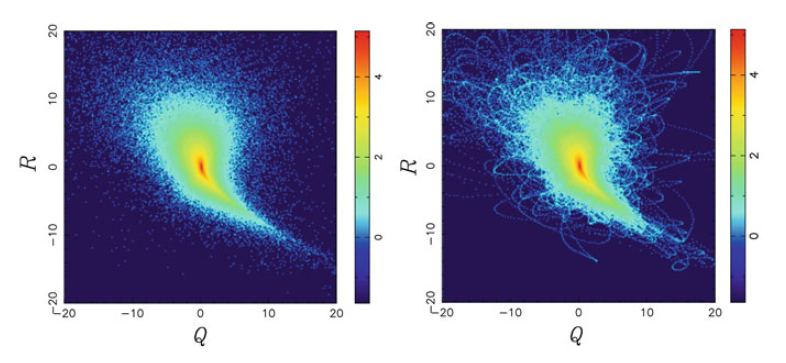
\includegraphics[scale=0.60]{tearDrop}
	\end{center}
	\caption{Distribuciones de probabilidad conjuntas de las invariantes $R$ y $Q$. En la izquierda se muestra la distribución de una serie de tiempo, en la derecha la distribución espacial para un solo tiempo. Esto ha sido utilizado como argumento a favor de la ergodicidad \parencite{galanti2000}.}
	\label{fig-tearDrop}
\end{figure}

Aparte de ésta aparente universalidad, también se ha observado que la vorticidad tiende a  alinearse con el segundo vector propio de la deformación \parencite{elsinga2010} (que posee un valor promedio cercano a cero, pero con grandes variaciones \parencite{hamlington2008}), contrario a lo que uno esperaría (que se alinee con el vector propio de mayor valor). En la figura \ref{fig-align} se muestra un ejemplo de la distribución de probabilidad de los ángulos (en este caso los cosenos de éstos) de la vorticidad con los vectores propios de la deformación.  

\begin{figure}[H]
	\begin{center}
		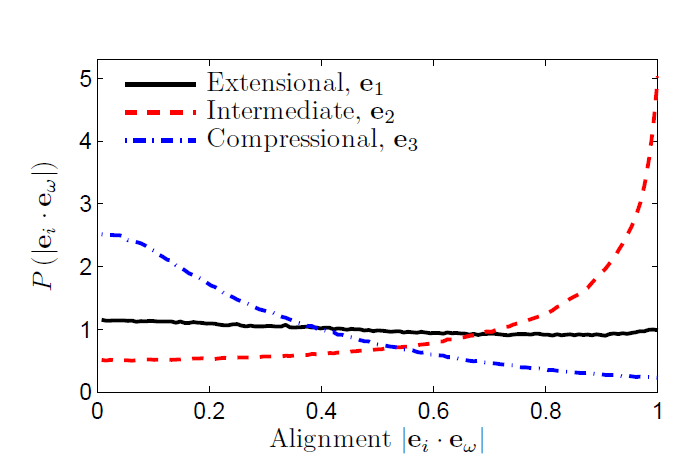
\includegraphics[scale=0.65]{strainAlignement}
	\end{center}
		\caption{Distribución de probabilidad de los ángulos entre la vorticidad y los vectores propios de la deformación,  \parencite{hamlington2008}. Se observa una alineación predominante de la vorticidad con el vector propio intermedio (curva roja en la figura).}
	\label{fig-align}
\end{figure}



\section{Estadística}

La turbulencia ha sido ampliamente estudiada desde un punto de vista estadístico \parencite{monin1976}, es la teoría más exitosa y también la más útil. Sin embargo es natural preguntarse ¿por qué necesitamos una descripción estadística de la turbulencia, o de los sistemas físicos deterministas en general?. La respuesta puede consistir de dos partes que están ligadas entre sí. La primera es que a la hora de estudiar un sistema físico no tenemos una certidumbre total sobre las condiciones iniciales/de frontera, esto naturalmente introducirá incertidumbre a los resultados medidos y provocará diferencias a la hora de compararlos con resultados teóricos. La segunda razón es que existen sistemas llamados caóticos que tienen una gran sensibilidad a las condiciones iniciales, es decir, un pequeño cambio en estas generará una gran diferencia en los resultados. Al unir ambos hechos vemos que una opción es dar una descripción estadística de los sistemas caóticos, ahora por lo tanto debemos entender como construir los elementos que forman ésta teoría.\\

Ahora que de alguna forma sabemos el 'por qué' la necesitamos, debemos desarrollarla, primero nos preguntamos qué es una probabilidad? Es una medida, esto se entiende mejor al pensar en eventos o procesos estocásticos (es decir, no deterministas). Supongamos que tenemos una variable aleatoria, digamos $u$, en una serie de tiempo, como se muestra en la figura.

\begin{figure}[H]
	\begin{center}
		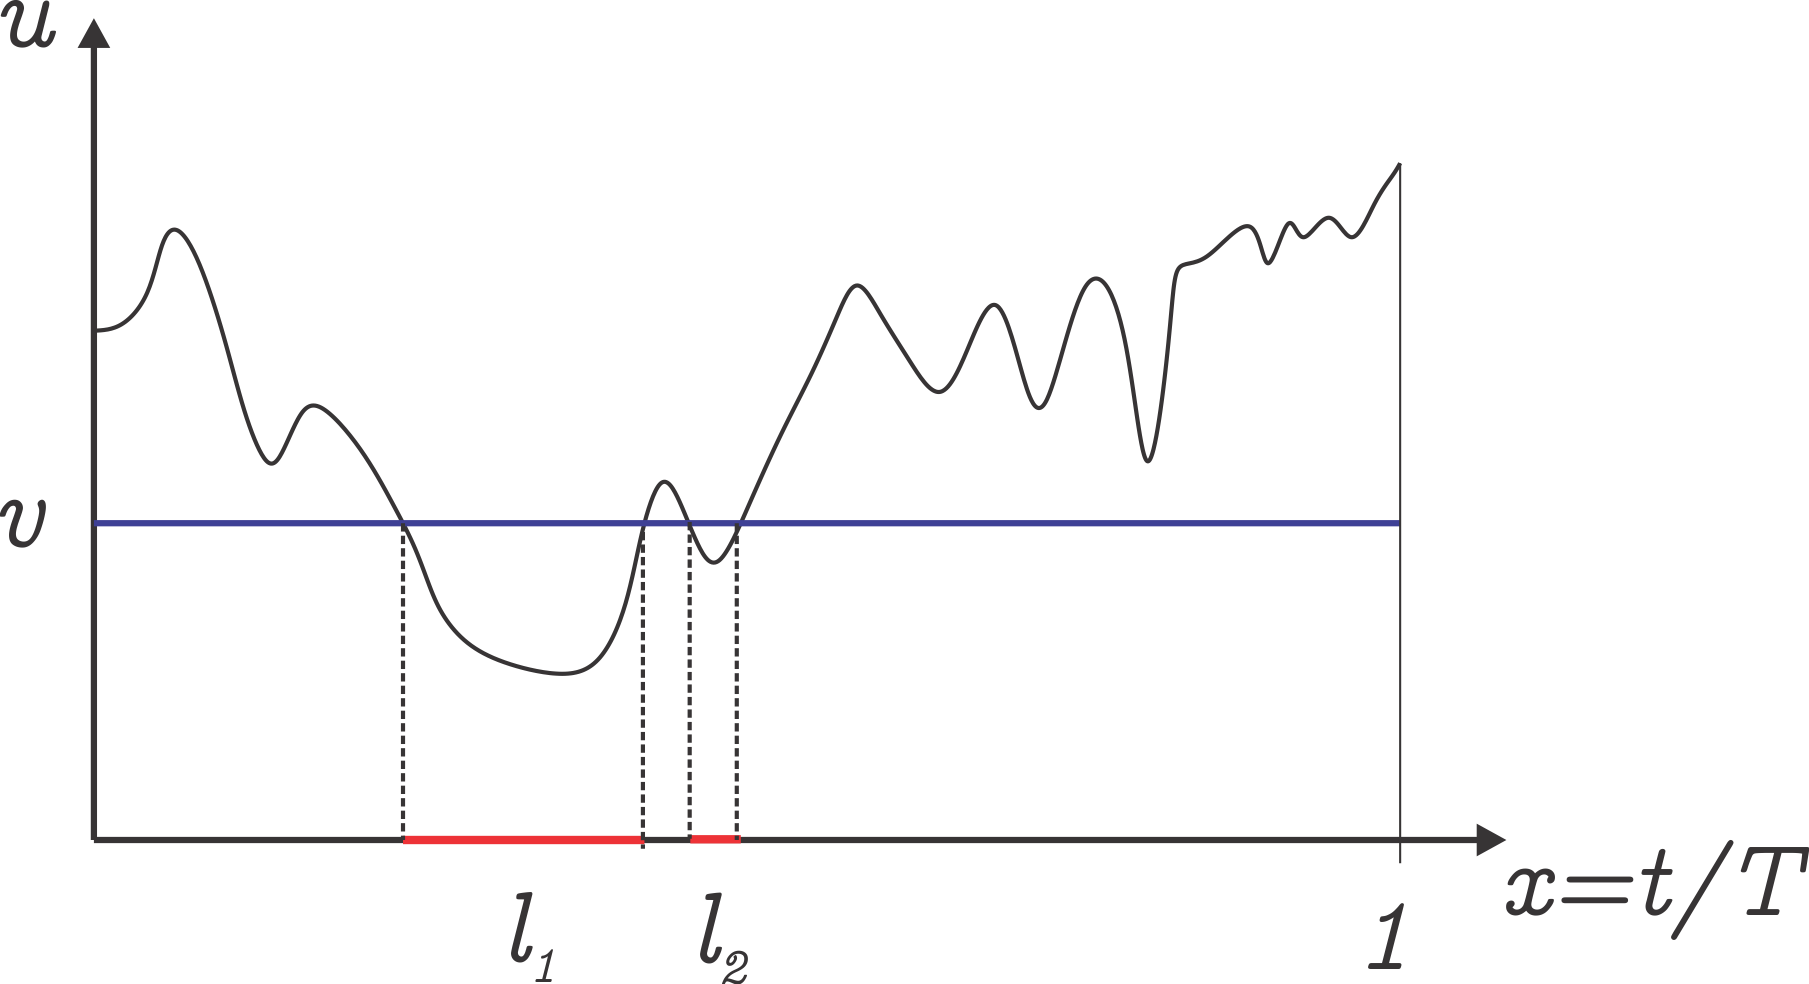
\includegraphics[scale=0.9]{probabilidad1}
	\end{center}
	\caption{Probabilidad como la medida de un conjunto.}
	\label{fig-prob1}
\end{figure}


Entonces nos preguntamos: Si seleccionamos $n$ instantes de tiempo al azar, cuantas veces el valor de $u$ sea menor a cierto valor $v$?  En este sentido la probabilidad es una medida, dado que se puede identificar con la razón entre la cantidad de veces que se cumple la condición y el total de veces que ocurre algo, en el caso continuo (como en la figura \ref{fig-prob1}) por lo tanto es la razón entre los intervalos que cumplen la condición y los que no. Si normalizamos el eje $x$ según el tiempo total de la serie, entonces podemos caracterizar la probabilidad como el tamaño (la medida) de los subconjuntos de $[0,1]$ que cumplen cierta condición, 

\begin{equation}
	Pr\left\{u< v\right\}=\mu\left\{x\rvert u< v\right\}
\end{equation} 
          
Donde $\mu$ es llamada una medida, que intuitivamente es una forma de identificar el conjunto con un tamaño \footnote{Para más información sobre teoría de la medida y probabilidad se pueden consultar los textos de Lumley \parencite{lumley2007} o Lasota \parencite{lasota2013}, por ahora no adentraremos más en estos aspectos matemáticos sin embargo algunos resultados como el teorema de Radon-Nikodym son importantes para el estudio de sistemas dinámicos}. En el ejemplo de la figura, 
\begin{equation}
	Pr\left\{u< v\right\}=l_1 + l_2
\end{equation}
Ésta definición de probabilidad es simplemente una generalización del caso discreto, donde la probabilidad de que ocurra un evento entre otros $N$ será,

\begin{equation*}
	Pr\left\{u\leq u_c\right\}=\frac{n(u< v)}{N} 
\end{equation*}
Es decir, la razón entre el número de eventos donde $u\leq v$ y la cantidad total de eventos $N$. Ahora podemos introducir una función que nos describa la probabilidad,

\begin{equation}
	F(v)=Pr\left\{u< v\right\}=\mu\left\{x\rvert u< v\right\}
\end{equation} 
la cual es conocida como función de probabilidad acumulada. Podemos identificar de inmediato las propiedades de ésta función (en la figura podemos observar la forma típica de ésta función): 
\begin{itemize}
	\item Debe ser monotona creciente, dado que si tenemos $F(v_1)=Pr\left\{u< v_1\right\}$ y $F(v_2)=Pr\left\{u< v_2\right\}$ con $v_2>v_1$, es claro que $F(v_2)\geq F(v_1)$, el intervalo asociado a la segunda probabilidad es al menos tan grande como el asociado a la primera. 
	\item La probabilidad  $F(v)$ cuando $v\to -\infty$ debe ser $0$, esto es válido para cantidades físicas, pero pueden tomar un valor infinito en un conjunto de medida $0$ sin afectar ésta propiedad (en el conjunto $[0,1]$ un subconjunto de medida $0$ es por ejemplo el de los números racionales).
	\item La probabilidad $F(v)$ cuando $v \to \infty$ debe ser $1$. 
	\item Dado que $F(v)=	Pr\left\{u< v\right\} = \mu\left\{x\rvert u< v\right\}$, $F(v)\geq 0$, ésta es una propiedad de la medida $\mu$, pero también es intuitivo que no puede existir una probabilidad negativa. 
\end{itemize}

\begin{figure}[H]
	\begin{center}
		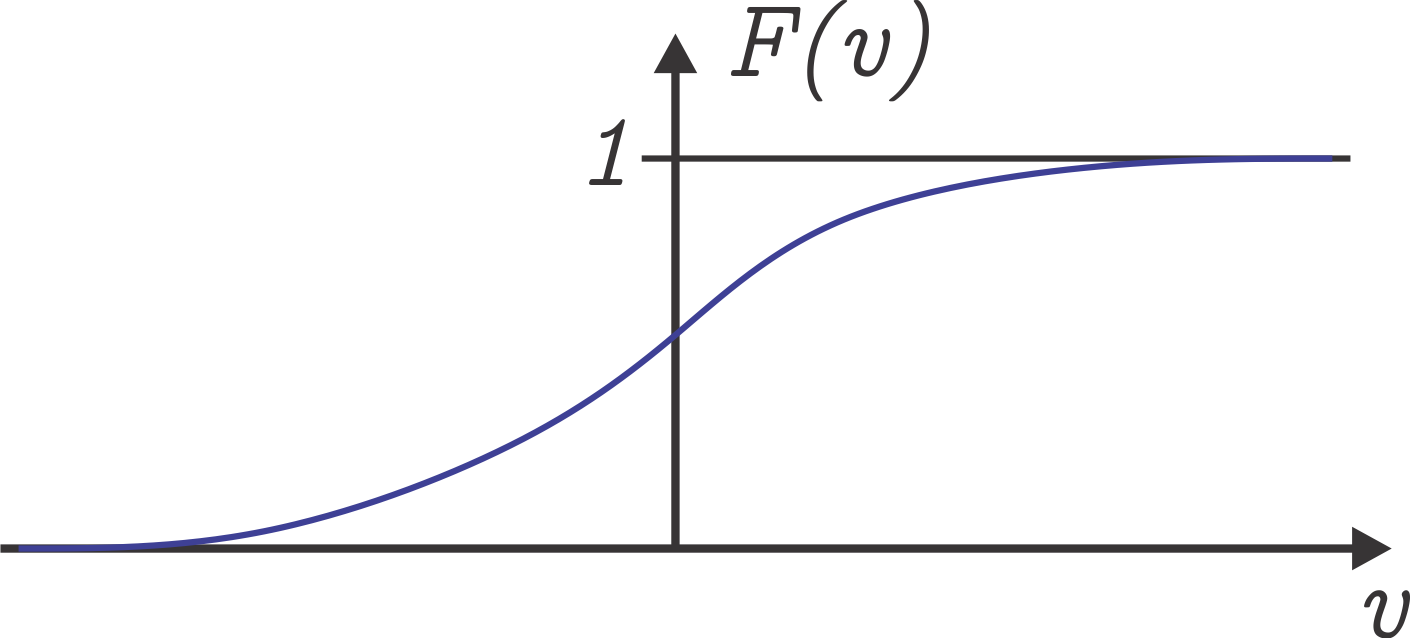
\includegraphics[scale=1]{probabilidad2}
	\end{center}
	\caption{Forma típica de $F(v)$.}
	\label{fig-prob2}
\end{figure}

Ahora consideremos el caso en que queremos determinar la probabilidad $Pr\{ v_1 <  u < v_2 \}$, entonces tenemos,

\begin{equation}
	Pr\{ v_1 <  u < v_2 \} = \mu \{v_1 <  u < v_2 \}=\mu\{ u < v_2 \} - \mu\{ u < v_1 \} =F(v_2)-F(v_1) 
\end{equation}
Donde se utiliza la propiedad de la medida de probabilidad (que está normalzada a 1 dado que la probabilidad total es 1) $\mu(A-B)=\mu(A)-\mu(B)$ \parencite{billingsley2008}. A partir de esto también nos podemos preguntar cual es la probabilidad de encontrar el valor de la variable $u$ en un intervalo infinitesimal $[u,u+du]$, la respuesta a esto está dada por la función de densidad (cuya existencia está garantizada bajo ciertas condiciones por el teorema de Radon-Nikodym) $\rho(u)$. Con ésta función podemos expresar la probabilidad de un subconjunto $A$ del espacio de muestra (espacio donde $u$ toma los valores) según,

\begin{equation}
	Pr\{ A \}=\nu\{A\}=\int_{A} \rho(v) \mu (dv)
\end{equation} 
Donde $\nu$ es otra medida construida a partir de la medida $\mu$. Generalmente $\mu$ se puede tomar como la medida de Lebesgue (que coincide con la noción usual de volumen en $\mathbb{R} ^n$, $n \in \{1,2,3\}$). La función $\rho(u)$ también se conoce como la derivada de Radon-Nikodym y se escribe como, 

\begin{equation*}
	\derivative{\nu}{\mu}=\rho(v)
\end{equation*}
 
O en términos de la función de probabilidad acumulada $F(v)$,

\begin{equation}
	\rho(v)=\frac{dF}{dv}
\end{equation}
 
Para que $\rho(v)$ sea una densidad de probabilidad debe cumplir ciertas propiedades, teniendo en cuenta que la probabilidad de encontrar $u$ entre dos valores está dada por,
\begin{equation}
	Pr\{v_1<u<v_2\} = \int_{v_1}^{v_2} \rho(v) dv
\end{equation}
Entonces podemos identificar las siguientes propiedades
\begin{itemize}
	\item La función debe ser positiva, $\rho(v)\geq 0$
	
	\item Debe estar normalizada, es decir, la probabilidad total debe ser $1$,  $\int_{-\infty}^{\infty} \rho(v) dv =1$, por lo tanto $\lim_{v\to\infty} \rho(v)=\lim_{v\to-\infty}\rho(v)=0$
\end{itemize}


Para comprender mejor los conceptos anteriores vamos a poner un ejemplo. Consideremos un oscilador armónico simple, 

\begin{equation*}
	x(t)=A\sin\omega t
\end{equation*}

Si seleccionamos tiempos al azar, cual es la probabilidad de obtener algún valor de $x(t)$? Recordando el concepto de medida, el tamaño de un intervalo infinitesimal (normalizado a $[0,1]$) estará dado por,

\begin{equation}
	dl=\frac{dt}{T}
\end{equation} 
Donde $T$ se puede considerar como el periodo, $T=2\pi/\omega$. Además tenemos que,

\begin{equation}
	t(x)=\frac{1}{\omega}\arcsin\left(\frac{x}{A}\right)
\end{equation}

Por lo tanto, 

\begin{equation}
	dt=\frac{1}{A\omega}\frac{d}{dx}\left[\arcsin\left(\frac{x}{A}\right)\right]dx=\frac{1}{\omega}\frac{1}{\sqrt{A^2-x^2}} dx
\end{equation}
Entonces tenemos que,
\begin{equation*}
	dl=\frac{dt}{T}=\frac{1}{2\pi}\frac{1}{\sqrt{A^2-x^2}} dx
\end{equation*}
Y la densidad de probabilidad está dada por (correctamente normalizada),
\begin{equation}
	\rho(x)=\frac{1}{\pi}\frac{1}{\sqrt{A^2-x^2}}
\end{equation}
 En la figura \ref{fig-prob3} podemos observar la forma de esta función (para $A=1$). Un aspecto interesante de la función es que $\rho \to \infty $ en los extremos, esto se debe a que la velocidad en estas posiciones es $0$, por lo que es más probable encontrar el oscilador en estas posiciones. Esto se refleja en la función de probabilidad acumulada (figura \ref{fig-prob3} derecha) como puntos donde no es derivable. Además notemos que las unidades de la densidad deben ser $\frac{1}{m}$ para que la probabilidad sea adimensional.\\
 
 A partir de las funciones  
  
 \begin{figure}[H]
 	\begin{center}
 		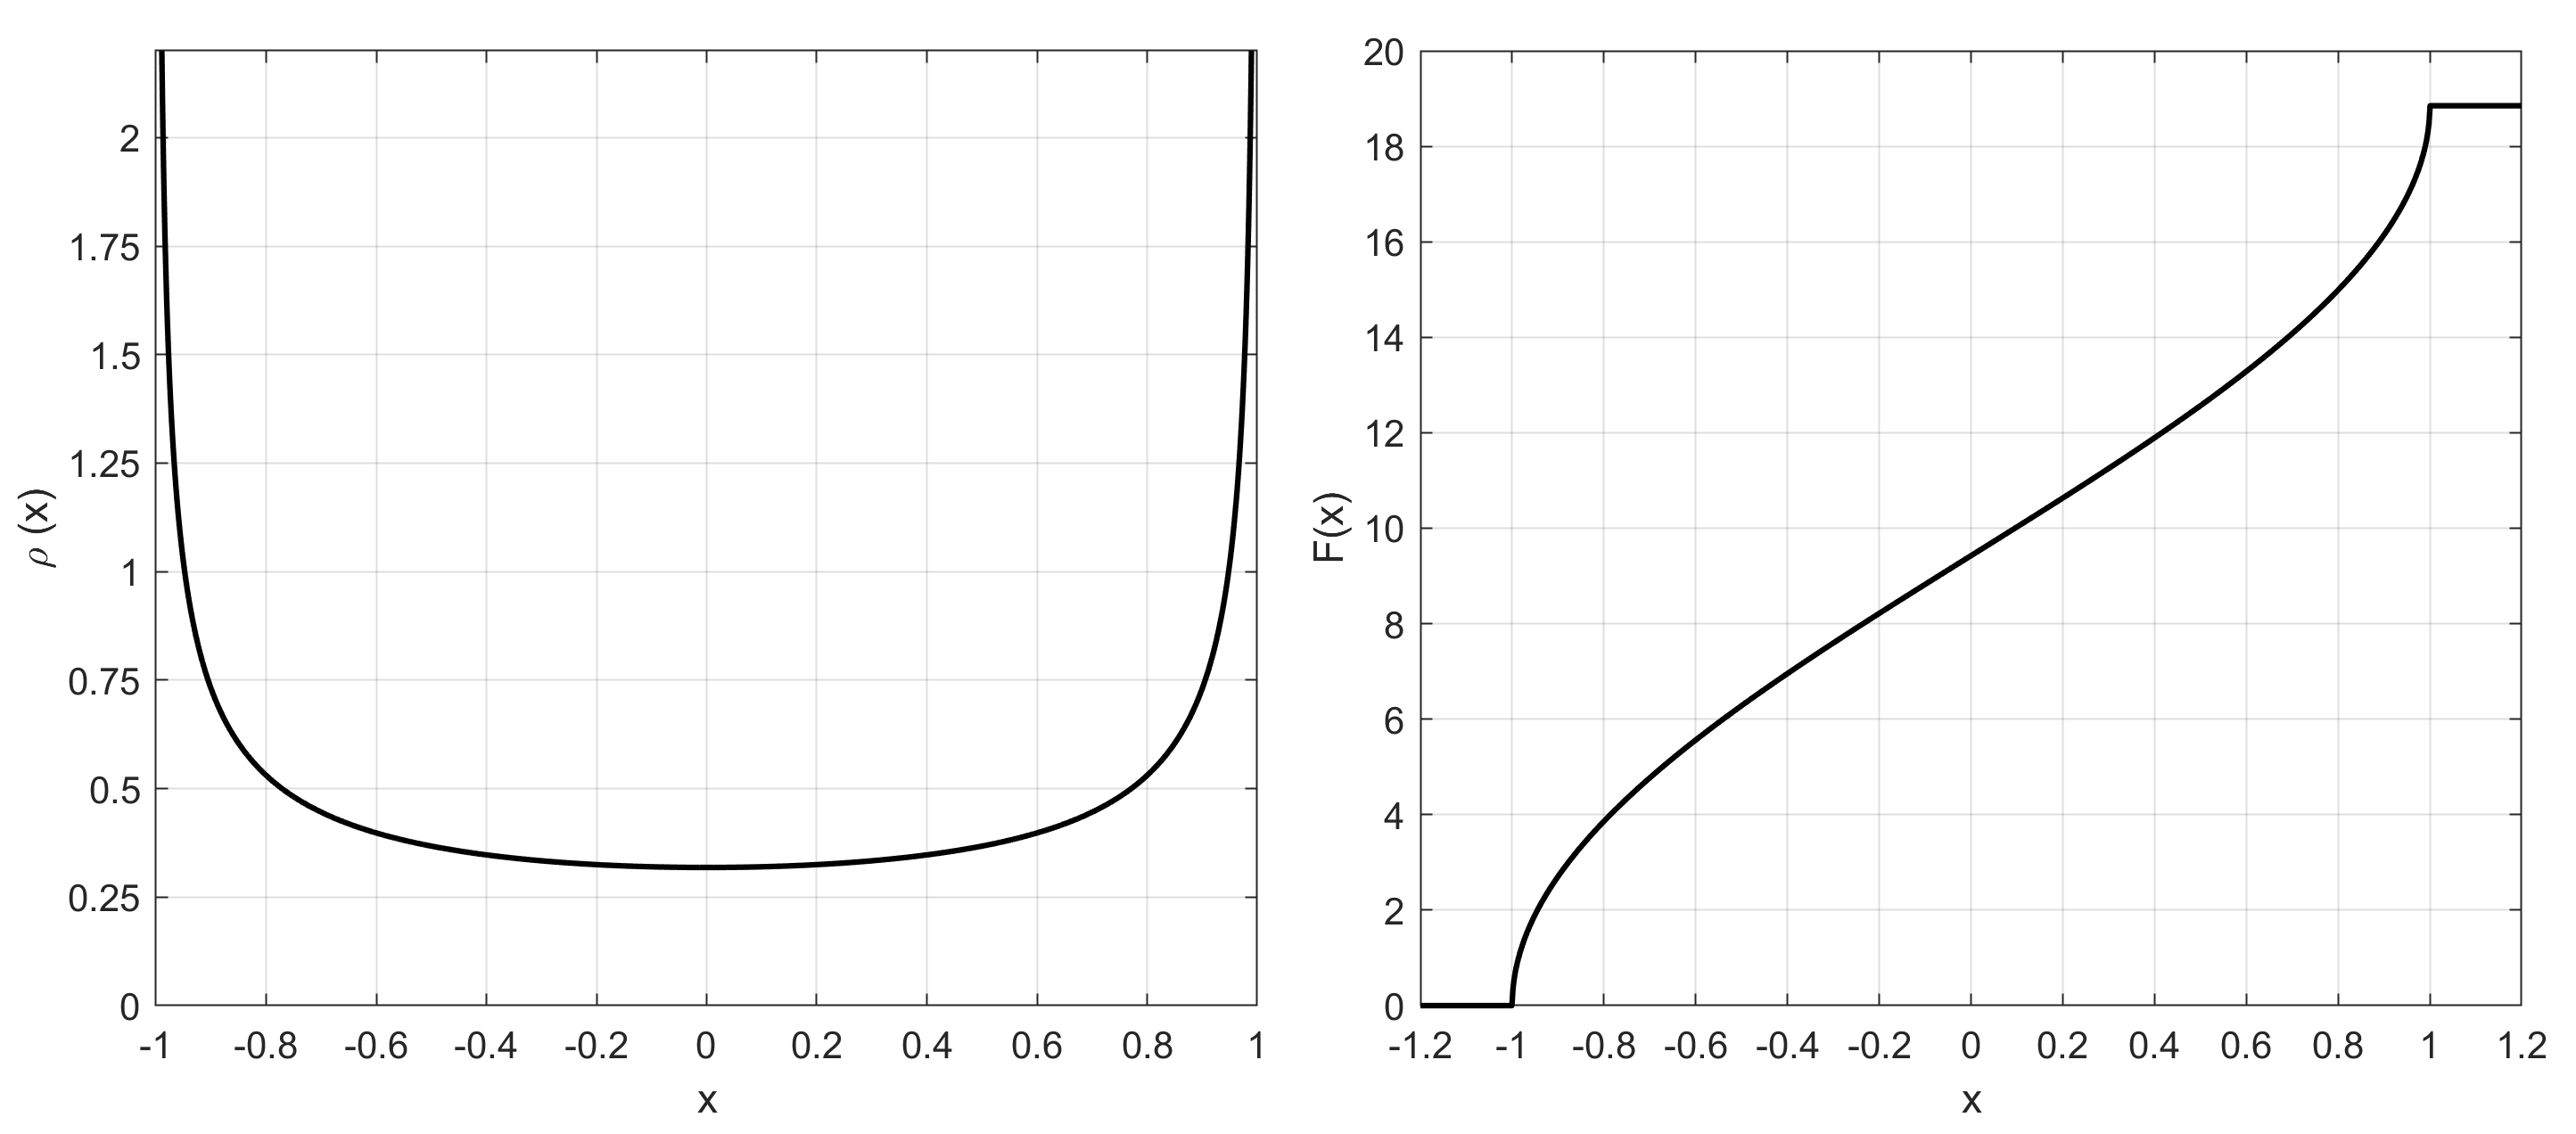
\includegraphics[scale=0.6]{probabilidad3}
 	\end{center}
 	\caption{Función de densidad (izquierda) y probabilidad acumulada (derecha), oscilador armónico clásico con $A=1$.}
 	\label{fig-prob3}
 \end{figure}
 
 \subsection{Momentos}
 
A partir de la función de densidad de probabilidad podemos derivar diferentes cantidades de interés para la descripción estadística de un sistema. Dada una función de la variable aleatoria $V$, $f(V)$, su valor esperado o valor medio está dado por,


\begin{equation}
	E\{ f(U) \}=\langle f(U) \rangle = \int_{-\infty}^{\infty} f(V) \rho(V)dV 
\end{equation}
 En la expresión anterior se muestran las dos notaciones más utilizadas. De particular interés son los momentos de la variable. El momento de orden $n$ se define como,
 
\begin{equation}
	\mu_n=\langle U^n \rangle = \int_{-\infty}^{\infty} V^n \rho(V)dV 
\end{equation} 
 
 En la tabla se muestran los nombres de algunos momentos más utilizados. El momento de primer orden es conocido como el valor medio, está dado por,
 \begin{equation}
 	\mu_1=\langle U\rangle=\int_{-\infty}^{\infty} V \rho(V)dV 
 \end{equation}
 
 Y la variable aleatoria $u$ se dice centrada (también llamada la fluctuación) si su valor medio es nulo. Dada una variable aleatoria $U$, esta se puede centrar restandole su valor medio y definiendo $u=U-\langle U\rangle$, dado que 
 
 \begin{equation*}
 	\langle u\rangle=\langle U-\langle U\rangle\rangle= \int_{-\infty}^{\infty}( V-\langle U\rangle )\rho(V)dV =\langle U \rangle - \langle U \rangle =0
 \end{equation*}
 
 El segundo momento de la variable centrada $u$ es conocido como la varianza y generalmente se identifica con $\sigma^2 $, 
 
 \begin{equation}
 	\sigma^2= \langle u^2\rangle= \int_{-\infty}^{\infty} u^2 \rho(V)dV
 \end{equation}

La raiz de la varianza es llamada desviación estándar, $\sigma = \sqrt{\sigma^2}$. Podemos notar que, 

\begin{align*}
	\sigma^2 &= \int u^2 \rho(V)dV\\
	&=\int (V-\langle U \rangle)^2  \rho(V)dV \\
	&= \langle U^2 \rangle - 2\langle U\rangle^2 + \langle U\rangle^2\\
	&= \langle U^2 \rangle - \langle U\rangle^2\\
	&=\mu_ 2 -\mu_1 ^2 
\end{align*}

Los momentos en cierto sentido nos sirven para caracterizar la función de densidad $\rho$. Los impares nos entregan información sobre la simetría de la densidad (para densidades simétricas, estos momentos son cero), mientras que los momentos pares nos entregan información sobre las colas de esta, es decir, sobre la ocurrencia de eventos extremos. También es importante mencionar que se suele adimensionalizar los momentos según la desviación estándar, estos son llamados momentos estandarizados, 

\begin{equation*}
	\hat{\mu}_n=\frac{\mu_n}{\sigma^n}
\end{equation*}     

En la tabla se muestran los nombres dados a los primeros momentos. 
\begin{table}[H]
	\centering
	\begin{tabular}{ll}
	$\mu_1$	& Valor medio   \\
	$\mu_2$	& Varianza   \\
	$\mu_3$	& Skewness   \\
	$\mu_4$	& Kurtosis  
	\end{tabular}
\end{table}
 \subsection{Función característica}
 
 Se conoce como función característica a $G(k)$ dada por,
 \begin{equation}
 	G(k)=\int_{-\infty}^{\infty} e^{ikV} \rho(V)dV=\langle e^{ikU}\rangle
 \end{equation}
 Como podemos notar, esta función es la transformada de Fourier de la densidad. Un aspecto importante de ésta función es que podemos expandirla en series,
 
 \begin{equation*}
 	G(k)=\sum_n \frac{a_n}{n!} k^n
 \end{equation*}
 Los coeficientes $a_n$ son simples de determinar, simplemente derivamos con respecto a $k$, evaluamos en $k=0$ y obtenemos,
 \begin{equation*}
 	a_n=\int_{-\infty}^{\infty}(iV)^n\rho(V)dV=i^n\int_{-\infty}^{\infty}V^n\rho(V)dV=i^n \mu_n
 \end{equation*}
 Por lo tanto tenemos,
 \begin{equation}
 	G(k)=\langle e^{ikU}\rangle= \sum_n \frac{(ik)^n}{n!} \mu_n
 \end{equation}
 
Podemos ver que los coeficientes de la expansión en series de $G(k)$ corresponden a los momentos de la variable, generalmente a la función $G(t)=\langle e^{tU}\rangle$ se le llama función generadora de momentos debido a esta propiedad. 

\subsection{Estadística de varias variables}

Si consideramos, por ejemplo, el campo de velocidades de un fluido como variable aleatoria, entonces notamos que necesitamos describir 3 variables aleatorias, una por cada componente de la velocidad. En el caso más general de $n$ variables, la función de distribución acumulada está dad por,
\begin{equation*}
	F(V_1,...,V_n)=Pr\{U_1<V_n,...U_n<V_n\}
\end{equation*}  

Esta función posee las siguientes propiedades,

\begin{itemize}
	\item $\lim_{V_m\to\infty} F(V_1,...,V_m,...,V_n)=F(V_1,...,V_{m-1},V_{m+1},...,V_n)$ es decir, la función se independiza de la variable $V_m$ cuando $V_m\to\infty$, y cuando todas las variables tienden a infinito, la probabilidad es uno.
	\item  $\lim_{V_m\to\infty} F(V_1,...,V_m,...,V_n)=0$, la función tiende a cero cuando alguna de las variables tiende a $-\infty$.  
\end{itemize}

En analogía con lo realizado anteriormente, se define la densidad de probabilidad multivariable (también llamada conjunta) como,

\begin{equation}
	\rho(V_1,...,V_n)=\frac{\partial^n}{\partial_1...\partial_n} F(V_1,...,V_n)
\end{equation}

Las propiedades de esta función son,

\begin{itemize}
	\item $\rho(V_1,...,V_{m-1},V_{m+1},...,V_n)=\int \rho(V_1,...,V_m,...,V_n) dV_m$, a partir de ésta propiedad podemos obtener la densidad de una dimensión: $\rho(V_1)=\int...\int \rho(V_1,...,V_n) dV_2...dV_n $. 
	\item $\int... \int \rho(V_1,...,V_n) dV_1...dV_n=1$, es decir, la función deben estar normalizada.
\end{itemize}

Las funciones de densidad de una dimension obtenidas a partir de $\rho(V_1,...,V_n)$ son llamadas marginales. También se definen las funciones de densidad condicional como aquellas que nos indican la probabilidad de $(V_1,...,V_{m})$ tal que ocurra el suceso $(V_{m+1}=v_{m+1},...,V_{n}=v_n)$. El teorema de Bayes nos dice que ésta probabilidad condicional, denotada como $\rho(V_1,...,V_{m}\rvert V_{m+1}=U_{m+1},...,V_{n}=U_n)$ está dada por,

\begin{equation}
	\rho(V_1,...,V_{m}\rvert V_{m+1},...,V_{n})=\frac{\rho(V_1,...,V_n)}{\rho(V_{m+1},...,V_{n})}
\end{equation} 

Claramente la función de probabilidad condicional está normalizada, dado que,

\begin{align*}
	\int...\int \rho(V_1,...,V_{m}\rvert V_{m+1},...,V_{n}) dV_1...dV_m&=\int...\int \frac{\rho(V_1,...,V_n)}{\rho(V_{m+1},...,V_{n})} dV_1...dV_m\\
	&=\frac{\rho(V_{m+1},...,V_n)}{\rho(V_{m+1},...,V_{n})}\\
	&=1
\end{align*}
Ahora supongamos una distribución de 2 variables, $(V_1,V_2)$, estas variables se dicen independientes si,

\begin{equation*}
	\rho(V_1 \rvert V_2)=\rho(V_1)
\end{equation*}
es decir, el hecho de saber que $V_2=U_2$ toma algun valor no nos dice nada sobre la distribución de $V_1$. Del teorema de Bayes tenemos,

\begin{equation*}
	\rho(V_1\rvert V_2)=\frac{\rho(V_1,V_2)}{\rho(V_2)}=\rho(V_1)
\end{equation*}
Por lo que llegamos a la siguiente conclusión: si dos variables aleatorias son independientes su función de distribución conjunta está dada por el producto de sus marginales,

\begin{equation}
	\rho(V_1,V_2)=\rho(V_1)\rho(V_2)
\end{equation}

También podemos calcular los momentos de multiples variables, estos están dados por,

\begin{equation}
	\langle u_1^{m_1}... u_n^{m_n}\rangle = \int...\int (V_1-\langle U_1\rangle)^{m_1} ... (V_n -\langle U_n\rangle)^{m_n} \rho(V_1,...,V_n) dV_1...dV_n
\end{equation}

Slo el momento de la forma $\langle u_1...u_n\rangle$ tiene nombre, y la matriz formada por las combinaciones de estos momentos es llamada matriz de correlación,

\begin{equation}
	\langle u_i u_j \rangle = \int\int (V_i-\langle U_j\rangle) (V_i-\langle U_j\rangle) \rho(V_1,V_2) dV_1 dV_2
	\label{corr.func}
\end{equation}

\begin{equation*}
    C=\mqty[\langle u_1 u_1 \rangle & \langle u_1 u_2 \rangle \\ \langle u_2 u_1 \rangle & \langle u_2 u_2 \rangle]
\end{equation*}

Cuando las variables son independientes podemos descomponer la densidad como el producto de las marginales, de $\ref{corr.func}$ es simple ver que en este caso la matriz de correlación es diagonal ($\langle u_1 u_2\rangle=0$). Este termino normalizado por el segundo momento es llamado el coeficiente de correlación,

\begin{equation*}
	\rho_{12}=\frac{\langle u_1 u_2\rangle}{\sqrt{\langle u_1 ^2\rangle\langle u_2 ^2\rangle}}
\end{equation*}
En general, cuando tenemos una matriz de correlación de más dimensiones, los diferentes términos no-diagonales son los coeficientes de correlación $\rho_{ij}$, $i\neq j$. 

\subsection{Procesos aleatorios}

Hasta ahora hemos descrito el caso de variables aleatorias que no dependen del tiempo, que ocurre si tenemos una serie de tiempo aleatoria? En este caso la variable $U=U(t)$, toma un valor aleatorio  en cada instante de tiempo, por lo que la función de probabilidad acumulada también depende del tiempo,


\begin{equation*}
	F(V;t)=Pr\{U(t)<V\}
\end{equation*}

Notemos que no es la variable en el espacio de muestra ($V$) la que depende del tiempo, sino $U$. De la misma forma la función de densidad también dependerá del tiempo,
\begin{equation*}
	\rho(V;t)=\pdv{F(V;t)}{V}
\end{equation*} 

Sin embargo éstas funciones no son suficientes para describir un proceso aleatorio, recordemos que podemos interpretar la probabilidad como una medida de los eventos que satisfacen una cierta condición. Teniendo esto en cuenta podemos observar que es posible reordenar los datos y esto no cambiara la cantidad de eventos que satisfacen la condición, por lo tanto no cambiará la probabilidad. Un ejemplo de esto es mostrado en la figura \ref{fig-prob4}.


\begin{figure}[H]
	\begin{center}
		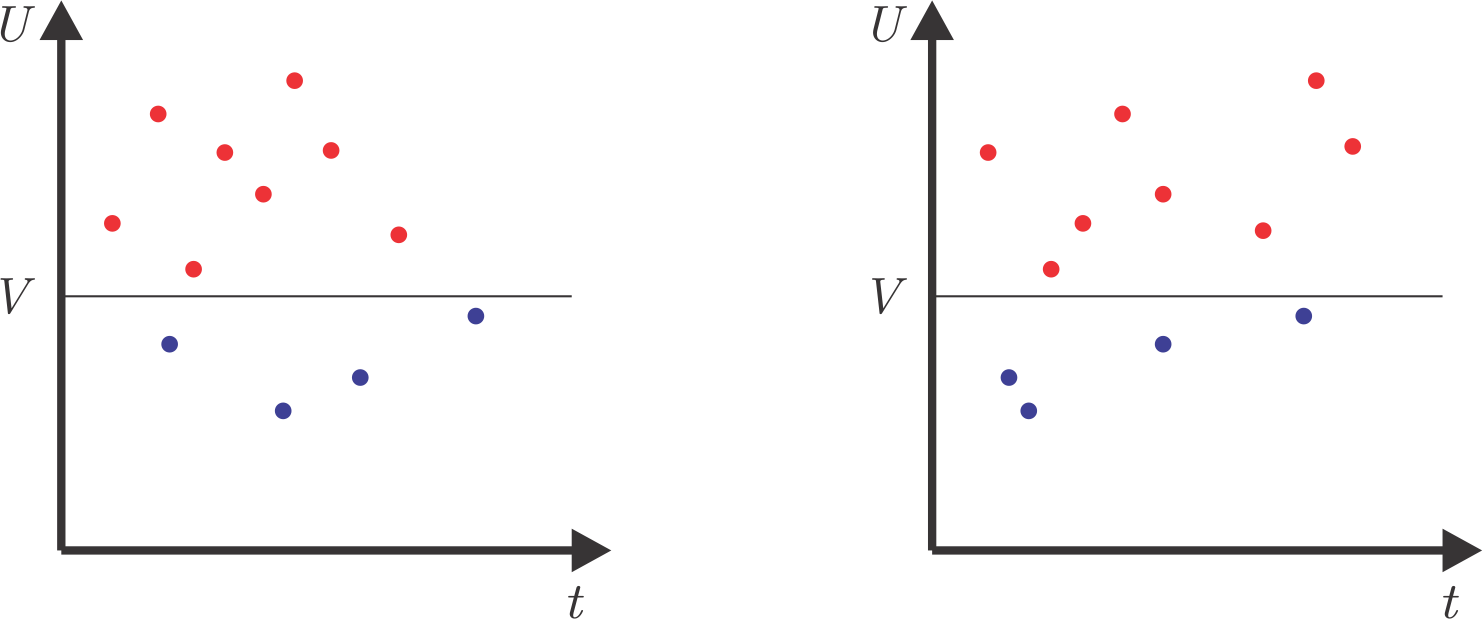
\includegraphics[scale=1]{probabilidad4}
	\end{center}
	\caption{En la figura se muestra una variable aleatoria medida en diferentes tiempos, podemos ver que en la derecha se reordenan los datos pero la probabilidad no cambia.}
	\label{fig-prob4}
\end{figure}

Entonces una pregunta natural es, como capturamos la estructura temporal de una proceso aleatorio? Para esto necesitamos una función de probabilidad de múltiples tiempos, en un caso ideal tendríamos la función de densidad en infinitos puntos. Para ver esto pensemos en la expansión en series de Taylor de la velocidad, la cual nos describe el comportamiento de la variable en una vecindad del punto, en ese caso necesitamos información sobre las derivadas de la variable $U(t)$, la derivada de primer orden está dada por,

\begin{equation*}
	U'(t)=\dv{U(t)}{t}=\lim_{h\to 0}\frac{U(t+h)-U(t)}{h}=\lim_{h\to 0} \left(\frac{1}{h}\right)U(t+h) + \left(-\frac{1}{h}\right)U(t)
\end{equation*}

Y podemos determinar sus momentos a partir de la función característica de dos variables (omitiendo el límite por ahora),

\begin{equation}
	\langle e^{i\frac{1}{h}U(t+h)-i\frac{1}{h}U(t)} \rangle=G\left(-\frac{1}{h},\frac{1}{h};t,t+h\right)
\end{equation}

Por lo que la estadística de la derivada está dada por,
\begin{equation}
	\langle e^{iU'(t)} \rangle=\lim_{h\to 0}\langle e^{\frac{1}{h}U(t+h)-\frac{1}{h}U(t)} \rangle=\lim_{h\to 0} G\left(-\frac{1}{h},\frac{1}{h};t,t+h\right)
\end{equation}

Entonces para la descripción estadística de la derivada necesitamos la función característica en dos puntos, de la misma forma para derivadas de mayor orden requerimos un mayor número de puntos ($n+1$ puntos para la derivada de orden $n$). Esto significa que para una descripción estadística completa en la vecindad de un tiempo necesitamos información sobre todas las derivadas, y por lo tanto se necesita la función de densidad de múltiples puntos. \\
Podemos también analizar la integral de un proceso aleatorio, 
\begin{equation*}
	I=\int_{a}^{b} U(t) dt
\end{equation*}   
Recordemos que la integral (de Riemann) puede escribirse como una suma de la forma,

\begin{equation}
	I=\lim_{n\to\infty} \sum_{k=0}^{n} U(p_k) \Delta_k t
\end{equation}

Donde $\Delta_k t =t_{k+1}-t_k$, con $t_0=a$ y $t_n=b$. Por lo tanto, podemos describir estadísticamente la integral de $U(t)$ (aproximada) por,

\begin{equation*}
	\langle e^{is\sum_{k=0}^{n} U(t'_{k}) \Delta_k t} \rangle = G(s\Delta_k t,...,s\Delta_n t;t'_{0},...,t'_{n}) 
\end{equation*}
Nuevamente observamos que para una descripción completa necesitamos un continuo de puntos en el intervalo de la integral. Ahora podemos introducir el llamado funcional característico, este contiene toda la información necesaria para describir un proceso aleatorio, es decir, información sobre las estadísticas de cualquier número de puntos. El funcional característico es definido por,


\begin{equation*}
	\mathcal{F}\left\{\vb{U}(\vb{x})\right\} = \int e^{\sum_i k_i x_i } U(\vb{x}) d\vb{x}
\end{equation*}

Una forma de ver esto es pensar en la transformada de Fourier de una cantidad, recordemos que está dada por,

\begin{equation}
	\Phi\left[U(t)\right]=\langle \langle e^{ i \int U(t) \theta(t)} dt \rangle \rangle
\end{equation}

Donde la suma es sobre todas las dimensiones, ahora si consideramos que este número de dimensiones tiende a infinito, reemplazamos la suma por una integral y recordamos que es la transformada de la función de densidad, es decir, las coordenadas ahora son las variables aleatorias $U(t_i)$ evaluadas en diferentes puntos, entonves vemos que en un sentido el funcional característico una transformada de Fourier de la densidad en un espacio de dimensión infinita (un espacio de funciones). \\

Ahora que tenemos una noción de lo que es un proceso aleatorio podemos estudiar sus estadísticas. Un proceso se dice estacionario si su función de densidad es invariante bajo translaciones temporales,

\begin{equation*}
	\rho(V_1,t_1+T;V_2,t_2+T;...;V_n,t_n+T)=\rho(V_1,t_1;V_2,t_2;...;V_n,t_n)
\end{equation*}

Es claro que la estacionariedad estadística no implica que el proceso en sí sea estacionario. Ahora podemos definir la autocovarianza como,
\begin{equation*}
	R(s)=\langle u(t)u(t+s)\rangle
\end{equation*}
Notemos que solo depende la diferencia entre ambos tiempos debido a la estacionariedad del proceso. Además se define la función de autocorrelación como,

\begin{equation*}
	\rho_t(s)=\frac{\langle u(t) u(t+s) \rangle}{\langle u^2(t)\rangle}
\end{equation*}

Una de las propiedades de un proceso estacionario es que su función de autocorrelación tiene simetría de paridad, esto se puede ver realizando el cambio $t'=t+s$, $R(s)=\langle u(t'-s)u(t')\rangle=R(-s)$. \\
En la figura \ref{fig-prob5} se observa un ejemplo, en la parte superior (a) se muestra la serie de tiempo de la velocidad de una simulación numérica directa en un flujo de Poseuille (está verificada la estacionariedad estadística). Los datos son obtenidos de la base de datos de la Universidad John Hopkins \footnote{Esta base de datos es constantemente actualizada con diferentes simulaciones, se puede acceder a ella desde: \href{http://turbulence.pha.jhu.edu}{http://turbulence.pha.jhu.edu}}  \parencite{li2008,lee2015}. En la figura \ref{fig-prob5}b) se muestra la función de autocorrelación en función de la variable $s$ (distancia temporal, tambien llamada \textit{lag}). 

\begin{figure}[H]
	\begin{center}
		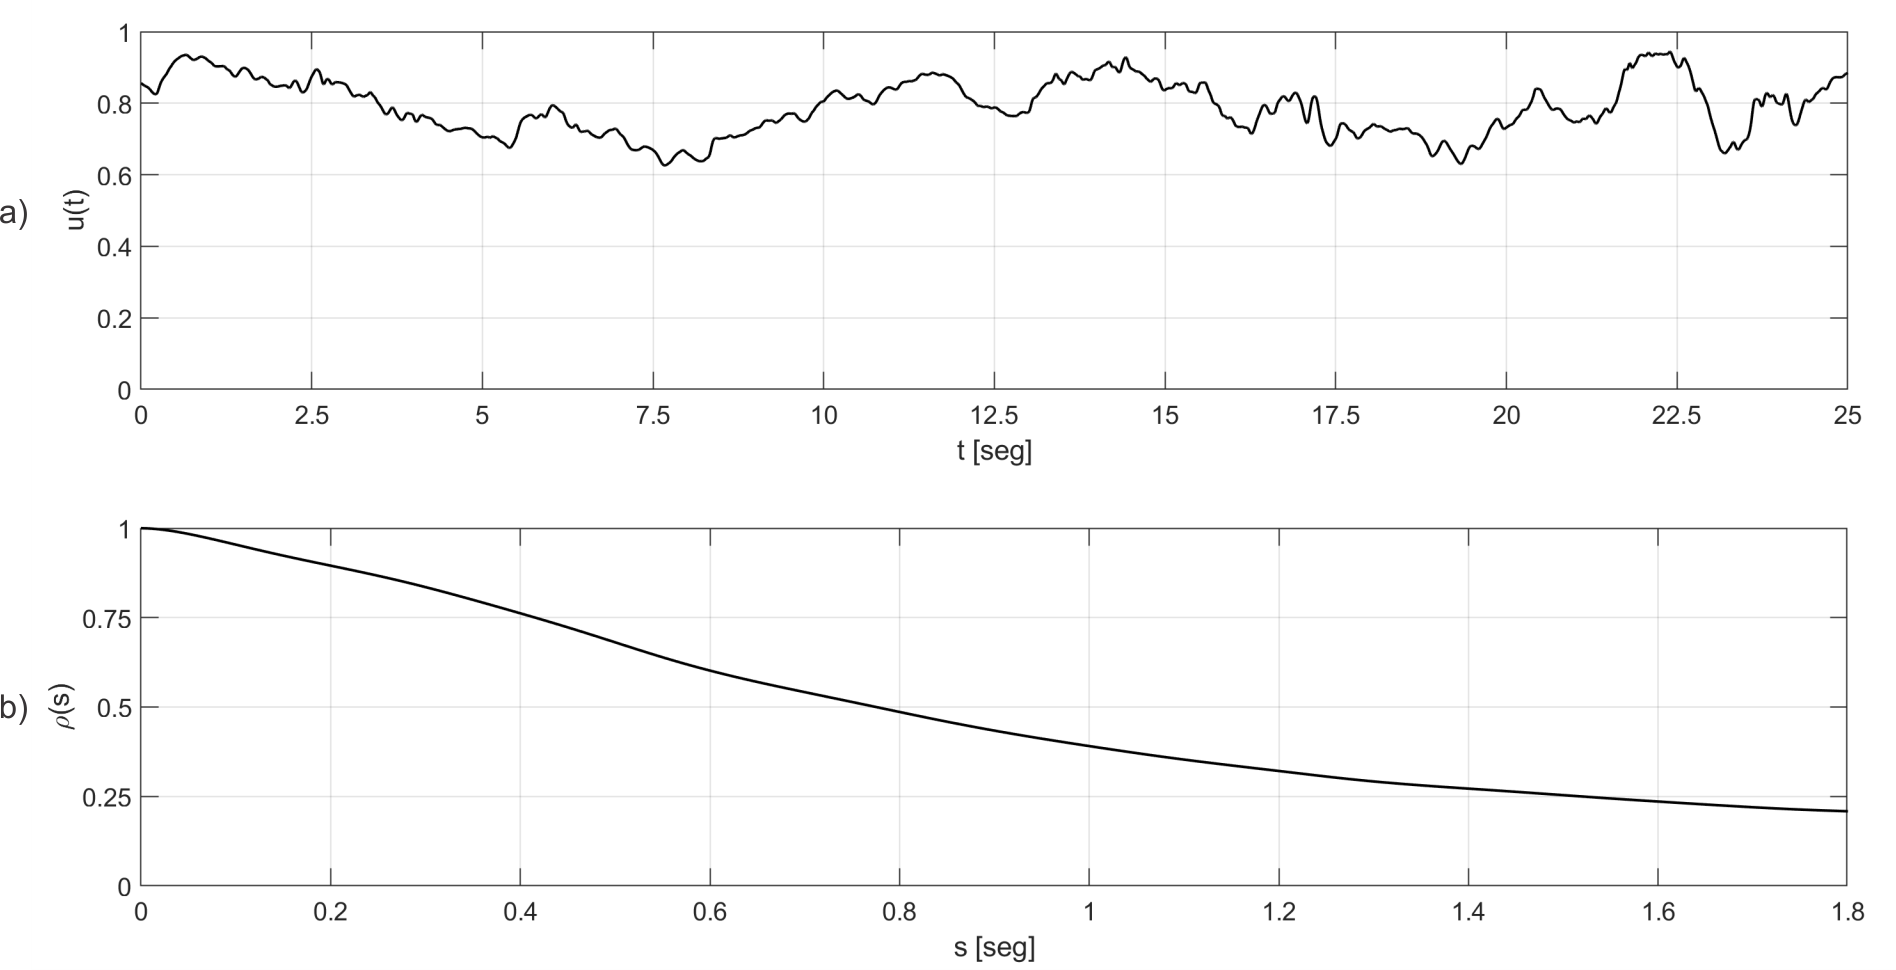
\includegraphics[scale=1]{probabilidad5}
	\end{center}
	\caption{Serie de tiempo de velocidad (datos de DNS de flujo de Poseuille). }
	\label{fig-prob5}
\end{figure}

También se define el tiempo de autocorrelación $\tau_c$ como,
\begin{equation}
	\tau_c=\int_{0}^{\infty} \rho_t(s) ds  
\end{equation}

esta es una medida de tiempo por sobre el cual se puede ignorar la correlación, es decir, cuando $s>\tau_c$, $\rho_t(s)\approx 0$. En la serie de tiempo mostrada en la figura \ref{fig-prob5} $\tau_c=0.94$ $[seg]$.\\


Si la variable aleatoria $u(t)$ es, por ejemplo, la velocidad, es claro que la función de correlación esta asociada a la energía cinética (por unidad de volumen) $E=\langle u^2 \rangle =R(0)$, por lo tanto el espectro de frecuencias de la variable $u(t)$ está dado por la transformada de Fourier de $R(s)$, 

\begin{equation*}
	E(\omega)=\frac{2}{\pi}\int_{0}^{\infty}e^{-i\omega s} R(s) ds  
\end{equation*}

Y la función de correlación se relacion con el espectro mediante,
\begin{equation*}
	R(s)=\int_{-\infty}^\infty E(\omega)e^{i\omega s} d\omega
\end{equation*}


Un punto importante es que, si el proceso es estacionario, tenemos, 
\begin{equation*}
	R(s)=R(-s)
\end{equation*}
Por lo tanto,

\begin{align*}
	R(s)=&2\int_{0}^\infty E(\omega)e^{i\omega s} d\omega\\ 
	=&2\int_{0}^\infty E(\omega)e^{-i\omega s} d\omega=R(-s)
\end{align*}
Luego llegamos a,
\begin{equation*}
	\int_{0}^\infty E(\omega)\left(e^{i\omega s}-e^{-i\omega s}\right) d\omega=0
\end{equation*}
Es decir, $e^{i\omega s}$ es una función par, por lo que solo conservamos los términos del coseno y las transformaciones se reducen a, 

\begin{equation*}
	R(s)=2\int_{0}^\infty E(\omega)cos(\omega s) d\omega
\end{equation*}

\begin{equation*}
	E(\omega)=\frac{2}{\pi}\int_{0}^{\infty} cos(\omega s) R(s) ds  
\end{equation*}

Podemos ver que cuando $s=0$ tenemos, 

\begin{equation*}
	R(0)=\langle u^2(t) \rangle =2 \int_{0}^{\infty} E(\omega) d\omega
\end{equation*}

Podemos ver que la integral entre $[\omega_a , \omega_b]$ de $E(\omega)$ corresponde a la contribución de los modos entre esas frecuencias a la varianza $\langle u^2 (t) \rangle$. 


\subsection{Campos aleatorios}

Podemos generalizar aún más una variable aleatoria y considerar que también depende del espacio, en este caso es llamada un campo aleatorio. Si tenemos en cuenta, por ejemplo, un campo de velocidad $\vb{U}(\vb{x},t)$ su función de probabilidad acumulada estará dada por,
\begin{equation*}
	F(\vb{V};\vb{x},t)=Pr\left\{U_i(\vb{x},t)<V_i\right\}
\end{equation*}

Y la función de densidad de probabilidad,

\begin{equation*}
	\rho(\vb{V};\vb{x},t)=\frac{\partial ^3 F(\vb{V};\vb{x},t)}{\partial_1 \partial_2 \partial_1}
\end{equation*}
La cual en el caso más general puede depender de $N$ puntos espaciotemporales, $\rho(\vb{V}^{(1)};\vb{x}^{(1)},t^{(1)};...;\vb{V}^{(N)};\vb{x}^{(N)},t^{(N)})$ .En el caso de una variable aleatoria con 3 componentes, aunque en general podría tener cualquier cantidad. Vemos que en este caso el primer momento está dado por,

\begin{equation*}
	\langle \vb{U}(\vb{x},t) \rangle= \int \int \int _{-\infty}^{\infty} \vb{V}f(\vb{V};\vb{x},t)d\vb{V}
\end{equation*} 

En general éste valor medio puede depender del tiempo y el espacio. Así como un proceso aleatorio puede ser estacionario (lo que impone ciertas simetrias en la función de densidad), los campos aleatorios pueden ser estacionarios, homogeneos e isotropos. La propiedad de homogeneidad significa que la función de densidad es invariante bajo traslaciones, es decir (para la densidad de un punto), $\rho(\vb{V};\vb{x},t)=\rho(\vb{V};\vb{r},t)$. De la misma forma, el campo se dice isótropo cuando la densidad es invariante bajo rotaciones.\\

Ahora podemos estudiar las estadísticas del campo, en forma similar al caso de los procesos aleatorios, donde necesitabamos estadísticas de multiples tiempos para analizar la estructura temporal del proceso, ahora se requieren estadísticas de varios puntos para el estudio de la estructura espacial (o espaciotemporal, en el caso más general). El caso más simple es la función de correlación de dos puntos y un tiempo,

\begin{equation*}
	R(\vb{r},\vb{x},t)=\langle u(\vb{x},t)u(\vb{x}+\vb{r},t) \rangle
\end{equation*}    

O en el caso que la variable tenga múltiples componentes, tenemos un tensor de correlación,

\begin{equation*}
	R_{ij}(\vb{r},\vb{x},t)=\langle u_i(\vb{x},t)u_j(\vb{x}+\vb{r},t) \rangle
\end{equation*}

Notemos que en el caso de un campo homogeneo la función solo depende de $\vb{r}$, y si es isótropo solo existe dependencia del módulo, $r$. De forma similar al caso de un proceso aleatorio, en este caso podemos definir una distancia de correlación. Teniendo en cuenta que $R(0,\vb{x},t)=\langle u^2(\vb{x},t) \rangle$ entonces la distancia de correlación (tambien llamada escala integral) está dada por,

\begin{equation*}
	L(\vb{x},t)=\frac{1}{R(0,\vb{x},t)}\int_{0}^{\infty} R(\vb{r},\vb{x},t) d\vb{r} 
\end{equation*}
Notemos que en el caso más general, cuando la velocidad tiene múltiples componentes, tenemos varias distancias de correlación $L_{ij}(\vb{x},t)$. \\
También podemos estudiar el espectro de la correlación $R_{ij}(\vb{r},t)$. En el caso homogeneo entonces se define el tensor espectral como,


\begin{equation*}
	\Phi_{ij}(\vb{k},t)=\frac{1}{(2\pi)^3}\int_{0}^{\infty} e^{-i\vb{k}\cdot\vb{r}}R_{ij}(\vb{r},t) d\vb{r} 
\end{equation*}
    
cuya inversa es,
\begin{equation*}
	R_{ij}(\vb{r},t)=\int_{0}^{\infty} \Phi_{i,j}(\vb{k},t)e^{i\vb{k}\cdot\vb{r}}d\vb{k}
\end{equation*}

Notemos que cuando $\vb{r}=\vb{0}$ entonces $R_{ij}(\vb{0},t)=\langle u_i(\vb{x},t) u_j(\vb{x},t) \rangle$ \footnote{Si estudiamos un flujo turbulento, $u_i$ corresponde a la componente de la fluctuación de la velocidad y la diagonal de $R_{ij}(\vb{0},t)$ es la energía cinética turbulenta. En este contexto el tensor $R_{ij}(\vb{0},t)$ es también llamado tensor de esfuerzos de Reynolds}. 


\subsection{Procesos de Markov y ecuación maestra}

En las siguientes secciones introduciremos un tipo de procesos llamados markovianos, el estudio de estos eventualmente nos llevará a la derivación de la ecuación de Fokker-Planck. Estas herramientas son útiles dado que se han usado en diversos estudios de turbulencia \parencite{friedrich2011,friedrich1997,peinke2019,wu2020}. También existen diversos libros que sirven como introducción al tema \parencite{wio2013,van1992,nicolis2012}. Un proceso de Markov $x(t)$ satisface la siguiente relación para la probabilidad conjunta,

\begin{equation*}
	P(x_1,t_1;x_2,t_2)=P(x_2,t_2\rvert x_1,t_1)P_1(x_1,t_1)
\end{equation*}

O de forma más general,

\begin{align*}
	P_n(x_1,t_1,...,x_n,t_n)&=P(x_1,t_1)P_{n-1}(x_1,t_2,...,x_n,t_n\rvert x_1,t_1)\\
							&=P(x_n,t_n\rvert x_{n-1},t_{n-1})...P(x_2,t_2\rvert x_1,t_1)P(x_1,t_1)
\end{align*}
Es decir, este tipo de procesos está completamente determinado por $P_1(x_1,t_1)$ y $P(x_2,t_2\rvert x_1,t_1)$. También satisfacen la llamada ecuación de Chapman Kolmogorov,

\begin{equation*}
	P(x_3,t_3\rvert x_1,t_1)=\int P(x_3,t_3\rvert x_2,t_2)P(x_2,t_2\rvert x_1,t_1) dx_2
\end{equation*}

y para la probabilidad no-condicional se satisface una relación similar,
\begin{equation*}
	P(x_2,t_2)=\int P(x_1,t_1)P(x_2,t_2\rvert x_1,t_1) dx_1
\end{equation*}
Ahora, considerando $t_3=t_2+\delta t$ y el límite $\delta t \to 0$ podemos ver que,

\begin{align*}
	\lim_{\delta t \to 0}P(x_3,t_2+\delta t \rvert x_2,t_2)=\int P(x_3,t_2+\delta t \rvert x_2, t_2)P(x_2,t_2\rvert x_1,t_1) dx_2
\end{align*}
Pero en el límite se debe cumplir $\lim_{\delta t \to 0}P(x_3,t_2+\delta t \rvert x_2,t_2)=P(x_3,t_2\rvert x_2,t_2)$ por lo tanto,

\begin{align*}
	\lim_{\delta t \to 0}P(x_3,t_2+\delta t \rvert x_2,t_2)&=\int P(x_3,t_2+\delta t)P(x_2,t_2\rvert x_1,t_1)dx_2\\
	&=\int \delta(x_3-x_2)P(x_2,t_2\rvert x_1,t_1)dx_2\\
	&=P(x_3,t_2\rvert_1,t_1)
\end{align*}

Debido a esto consideramos una expansión de la forma,

\begin{equation*}
	P(x_2,t_2+\delta t)\left[1-A(x_2)\delta t\right] +\delta t W(x_3\rvert x_2)+\mathcal{O}(\delta t^2)
\end{equation*}

Donde $A(x_2)=\int W(x_3\rvert x_2)dx_3$ y $W(x_3\rvert x_2)$ es llamada la probabilidad de transición (por unidad de tiempo) de $x_2$ a $x_3$. Ahora reemplazando esta expansión en la ecuación de Chapman-Kolmogorov,

\begin{align*}
	P(x_3,t_2+\delta t\rvert x_1,t_1)&=\int P(x_3,t_2+ \delta t)P(x_3,t_2\rvert x_1,t_1)dx_2\\
	&= \int\left[\delta(x_3-x_2)(1-A(x_3)\delta t)+\delta t W(x_3\rvert x_2)\right]P(x_2,t_2\rvert x_1,t_1) dx_2\\
	&=(1-A(x_3)\delta t)P(x_3,t_1\rvert x_1,t_1)+\delta t \int W(x_3\rvert x_2)P(x_2,t_2\rvert x_1,t_1) dx_2 
\end{align*}

Reordenando los términos llegamos a,
\begin{align*}
	\frac{P(x_3,t_2+\delta t\rvert x_1,t_1) -P(x_3,t_1\rvert 
		x_1,t_1)}{\delta t}&=-A(x_3) P(x_3,t_2\rvert x_1,t_1)\\
	& +\int W(x_3 \rvert x_2) P(x_2,t_2\rvert x_1,t_1) dx_2\\
	&=\int [W(x_3\rvert x_2) P(x_2,t_2\rvert x_1,t_1) \\
	&- W(x_2\rvert x_3)P(x_3,t_2\rvert x_1,t_1)]dx_2
\end{align*}
Donde se usó la definición de $A(x_3)$. Finalmente, en el límite llegamos a,



\begin{equation*}
	\partial_t P(x,t\rvert x_0,t_0)=\int \left[W(x,x')P(x',t'\rvert x_0,t_0)-W(x'\rvert x)P(x,t\rvert x_0,t_0)\right] dx'
\end{equation*}

Esta es conocida como ecuación Maestra, lo importante es que nos dice que en los procesos de Markov existe una perdida de memoria dado que la probabilidad en un tiempo $t+\delta t$ solo depende de las probabilidades en $t$, es decir, en el tiempo inmediatamente anterior. 

\subsection{Ecuación de Fokker-Planck}

Si en la ecuación maestra asumimos pequeñas variaciones en la variable aleatoria $x$, la probabilidad de transición decae rápidamente con $\abs{x-x'}$ \parencite{wio2013} y se escribe,



\begin{equation*}
	W(x\rvert x')=W(x',\xi) \hspace{0.5cm} \xi =x-x'
\end{equation*}

Luego la ecuación maestra es de la forma,
\begin{equation*}
	\partial_t P(x,t\rvert x_0,t_0)=\int \left[W(x-\xi,\xi)P(x-\xi,t'\rvert x_0,t_0)-W(x\rvert -\xi)P(x,t\rvert x_0,t_0)\right] d\xi
\end{equation*}

Se expande esta ecuación en $\xi$ llegando a,
\begin{align*}
	&\int \left[W(x-\xi,\xi)P(x-\xi,t'\rvert x_0,t_0)-W(x\rvert -\xi)P(x,t\rvert x_0,t_0)\right] d\xi\\
	=&\int [W(x,\xi)-\xi \partial_x W(x,\xi)+\xi^2 \partial_x^2 W(x,\xi)+...]P(x-\xi,t'\rvert x_0,t_0)d\xi \\
	& -P(x,t\rvert x_0,t_0)\int W(x\rvert -\xi)  d\xi
\end{align*}
El primer término de la expansión se anula con el último de la expresión anterior y se llama a la expansión,

\begin{equation*}
	\partial_t P(x,t\rvert x_0,t_0)=\sum_{n=1}^{\infty} \frac{(-1)^n}{n!}\partial^n_x \left[\alpha_n (x) P(x,t\rvert x_0,t_0)\right]
\end{equation*}

Esta es conocida como expansión de Kramers-Moyal y los coeficientes $\alpha_n(x)=\int \xi ^n W(x,\xi)d\xi$ son llamados coeficientes de Kramers-Moyal. Cuando los coeficientes tales que $n>2$ son despreciables entonces llegamos a la ecuación de Fokker-Planck,
\begin{equation*}
	\partial_t P(x,t \rvert x_0,t_0)=-\partial_x(\alpha_1(x)P(x,t\rvert x_0,t_0))+\frac{1}{2}\partial_x ^2(\alpha_2(x)P(x,t\rvert x_0,t_0))
\end{equation*}

Un resultado interesante de esta ecuación es que la evolución de la densidad de sistemas sobre los cuales actúa un ruido blanco obedece una ecuación difusiva (cuando los coeficientes son constantes). Por lo tanto, en estos casos, cuando comenzamos de una condición inicial concentrada en el espacio de fase, eventualmente la densidad se distribuye en el espacio. 

\subsection{Ecuación de Liouville}

Una pregunta natural es si, dada la evolución temporal de un sistema, es posible determinar una ecuación para la evolución de su densidad de probabilidad? La respues es que sí, el caso más conocido es en sistemas Hamiltonianos, donde las ecuaciones del movimiento tienen la forma,

\begin{equation*}
	 \dot{q}_i=\partial_{p_i} H \hspace{0.5cm} \dot{p}_i=-\partial_{q_i} H
\end{equation*} 

Estas variables se pueden expresar como un flujo en el espacio de fase $\vb{v}=[\dot{q}_1,...,\dot{q}_n,\dot{p}_1,...,\dot{p}_n]$. Ahora, sabemos que la probabilidad es una cantidad conservada (su integral en el espacio de fase siempre es $1$), por lo que su derivada temporal total debe ser nula y tenemos,

\begin{equation*}
	\frac{d \rho}{dt}=\partial_t \rho +\grad{}\cdot (\vb{v}\rho)=\partial_t +\rho\grad{}\cdot \vb{v} +\vb{v}\cdot\grad{} \rho =0
\end{equation*}
Donde el gradiente es sobre las coordenadas del espacio de fase, $\grad{}=[\partial_{q_1},...,\partial_{q_n},\partial_{p_1},..,\partial_{p_n}]$. Ahora en el caso de un sistema Hamiltoniano,

\begin{align*}
	\grad{}\cdot \vb{v}&=\partial_{\vb{q}} \cdot \dot{\vb{q}}+\partial_{\vb{p}}\cdot \dot{\vb{p}}\\
	&=\partial_{\vb{q}} \cdot \partial_{\vb{p}} H+\partial_{\vb{p}} \cdot \partial_{\vb{p}}\vb{r} H\\
	&=0
\end{align*}
Este resultado es importante, nos dice que los flujos Hamiltonianos son incompresibles. Esto no ocurre en flujos con disipación, los cuales son compresibles en el espacio de fase. 
Para el otro término tenemos,
\begin{align*}
	\vb{v}\cdot\grad{}\rho&=\dot{\vb{q}}\cdot\partial_{\vb{q}}\rho + \dot{\vb{p}}\cdot  \partial_{\vb{p}} \rho\\
	&=\partial_{\vb{p}}H\cdot \partial_{\vb{q}}\rho -\partial_{\vb{q}}H\cdot\partial_{\vb{p}}\rho
\end{align*}
Luego llegamos a la ecuación para $\rho$,

\begin{equation*}
	\partial_t \rho +\partial_{\vb{p}}\cdot \partial_{\vb{q}}\rho -\partial_{\vb{q}}H\cdot\partial_{\vb{p}}\rho=0
\end{equation*}
Esta es la ecuación de Liouville para sistemas Hamiltonianos, que se puede escribir en términos del bracket de Poisson como,
\begin{equation*}
	\left\{H,\rho\right\}=0
\end{equation*}

Si bien se usaron los sistemas Hamiltonianos como ejemplo, podemos obtener la ecuación de Liouville para cualquier sistema (la probabilidad siempre es conservada), solo debemos conocer su evolución temporal. En general, en términos del operador de Perron-Frobenius podemos escribir la evolución temporal de una densidad como,
\begin{equation*}
	\rho(\vb{x},t)=\int \delta\left[\vb{x}-\hat{\mathcal{L}\vb{x}_0}\right] d\vb{x}_0
\end{equation*}
Donde la integral es sobre las condiciones iniciales y el operador $\hat{\mathcal{L}}$ es el que dicta la evolución temporal de $\vb{x}(t)$. Se puede leer más sobre transporte de densidades en diversos libros \parencite{cvitanovic2005,lasota2013,gaspard2005,beck1995}.
	
\pagebreak
\section{Teoría de la información}

Para comenzar la siguiente discusión (basada en las referencias \parencite{nicolis2012,beck2009,cover1999}) debemos pensar en que es la información desde un punto de vista físico y que cantidades debemos analizar cuando la queremos estudiar. Si nos detenemos a pensar, la información está muy relacionada con la comunicación, es decir, en como la transmitimos. Las fundaciones de la teoría matemática de la comunicación fueron establecidas por Claude Shannon en 1948 \parencite{shannon1948}, sin embargo la teoría de la información se ha expandido a otras áreas y actualmente es aplicada en diversos campos de estudio (teoría de la computación, física \parencite{jaynes1957}, estadística, entre otros). Como ésta no es una introducción a la teoría, en éste capítulo solo introduciremos algunos conceptos útiles para nuestros fines. 

        
\subsection{Entropía}

La información está muy relacionada con la probabilidad, pensemos en la ocurrencia de cierto evento, tenemos dos casos opuestos:

\begin{itemize}
	\item Si sabemos que el evento ocurrirá con total certeza, es decir $p=1$, entonces no ganamos información con dicho evento, pues sabiamos de antemano que iba a ocurrir y podríamos haber analizado sus efectos antes de que ocurriera. 
	\item Si un evento tiene una probabilidad muy cercana a $p=0$ de ocurrir, entonces cuando ocurra ganaremos mucha información, dado no esperabamos la ocurrencia de dicho evento. 
\end{itemize}

Esto puede ser cuantificado por una función $h(p)$ \parencite{beck2009}, tal que cumpla estas condiciones. Si tenemos un grupo de posibles eventos con probabilidades $p_i$ (que satisfacen la condición de normalización) entones la información media que obtenemos de esta secuencia es $\langle h(p) \rangle$, es decir (en el caso discreto),

\begin{equation*}
	I=\langle h(p) \rangle=\sum_i p_i h(p_i)
\end{equation*}

O en el caso continuo,

\begin{equation}
	I=\langle h(p) \rangle=\int \rho(V) h(\rho)dV
\end{equation}

Y la entropía se define como $S=-I$. La definición más conocida de información es cuando $h(\rho)=\log(\rho)$, la llamada entropía de Shannon (\parencite{shannon1948}) es definida como,
\begin{equation}
	S=-\int \rho(\vb{V})\log(\rho(\vb{V}))d\vb{V}
	\label{eq.shann}
\end{equation}
Donde la base del logaritmo define las unidades de medida (si es un logaritmo natural se llaman nats, cuando la base es 2 son llamados bits). Hay ciertas condiciones que la entropía de Shannon (o la información de Shannon), estos son los llamados axiomas de Khinchin y deben ser satisfechos para que una medida de información sea válida \parencite{khinchin2013},

\begin{itemize}
	\item La información $I$ solo depende de la probabilidad de los eventos.
	\item La distribución uniforme minimiza la información (o máximiza la entropía). 
	\item Un evento con probabilidad $0$ no nos entrega información, $I(p_1,...,p_n)=I(p_1,...,p_n,0)$. 
\end{itemize}

Existe un cuarto axioma, pero este es relajado según la medida de información usada y tiene que ver con la entropía condicional, concepto que vamos a introducir más adelante. 

\subsection{Entropía de Shannon, información mutua y entropía relativa}

Ahora nos enfocaremos en la medida del tipo \ref{eq.shann}. Primero, para hacer un enlace entre teoría de la información y física, volvamos al segundo axioma de Khichnin, sabemos que la entropía es maximizada por la distribución uniforme. Si tenemos un sistema con $N$ estados accesibles, la entropía será,

\begin{equation*}
	S=-\sum_{i=1}^N \frac{1}{N} \log(\frac{1}{N})=\log(N)
\end{equation*} 

En física estadística la entropía de Gibbs se define como,
\begin{equation*}
	S=-k_B\sum_{i=1}^N p_i \log(p_i)
\end{equation*}
Donde $k_B$ es la constante de Boltzmann, vemos que ésta definición coincide con la entropía de Shannon (solo se diferencian por la constante). En el caso de la distribución uniforme tenemos la entropía de Boltzmann,

\begin{equation*}
	S_B=-k_B \log(\Omega(E))
\end{equation*} 
Donde $\Omega(E)$ es el número de microestados accesibles con energía $E$. Más adelante veremos que al imponer distintas restricciones a la maximización de la entropía podemos obtener las distribuciones correspondientes a los otros ensambles encontrados en física estadística, sin embargo una ventaja de este enfoque es que el método no está limitado a sistemas en equilibrio termodinámico \parencite{beck2009,edwards1969}.\\

Un ejemplo muy simple del calculo de la entropía es el caso de una moneda (no cargada), sabemos que hay dos estados accesibles (cara y sello), cada uno con probabilidad $1/2$, por lo tanto la entropía es,

\begin{equation*}
	S=-\log(\frac{1}{2})=\log(2)
\end{equation*}
si el logaritmo es en base $2$, vemos que la entropía es $1 [bit]$. Un punto importante sobre la medida de información $h(p)=-p\log(p)$ es su concavidad en $[0,1]$, como podemos ver en la figura,


\begin{figure}[H]
	\begin{center}
		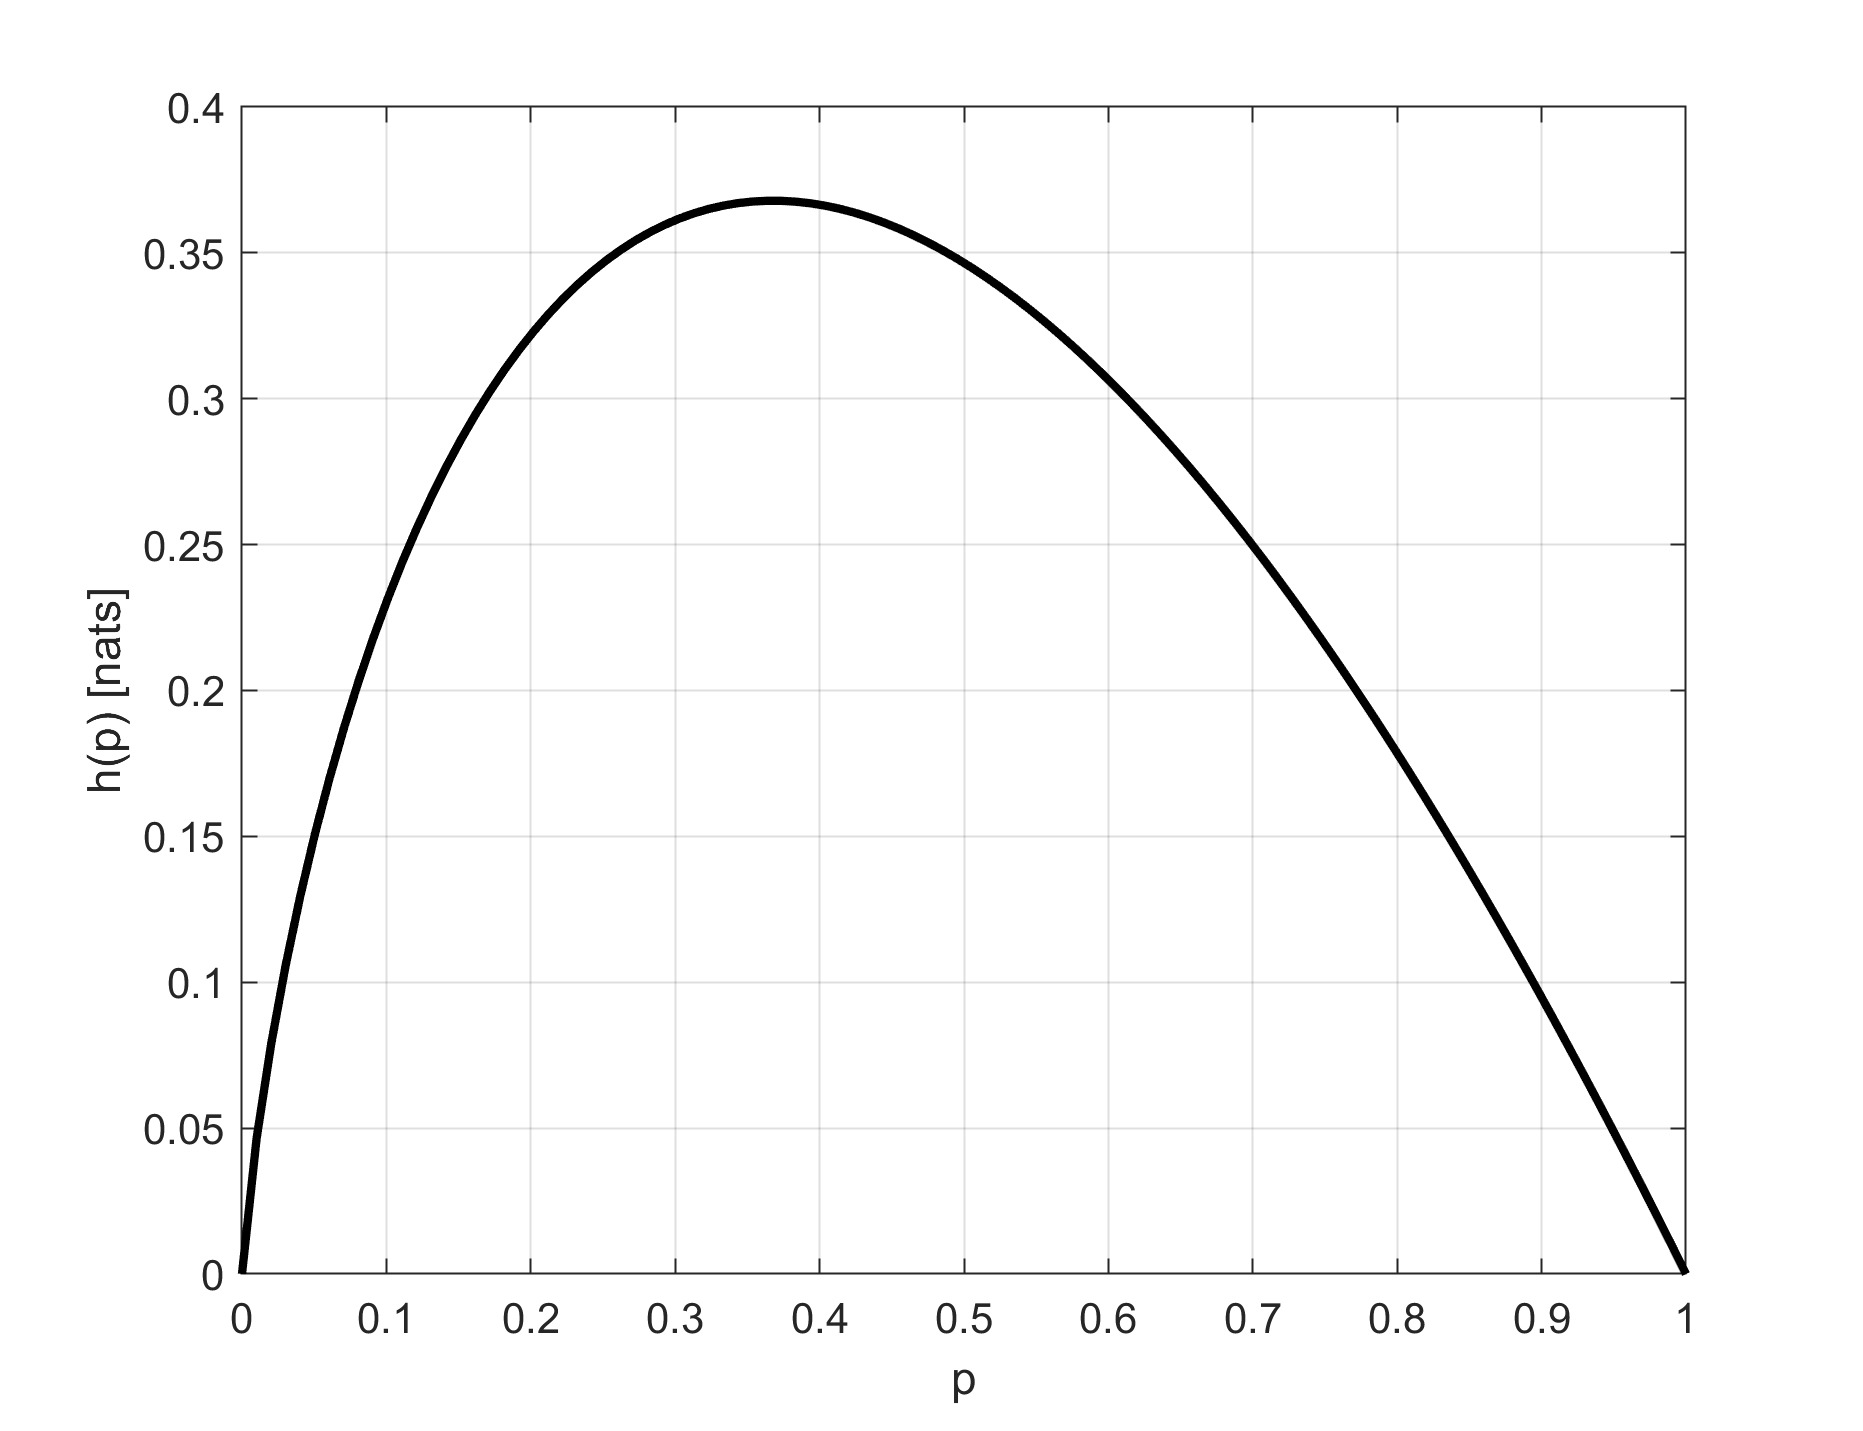
\includegraphics[scale=1]{entropyConc}
	\end{center}
	\caption{Gráfico de $h(p)=-p\log(p)$.}
	\label{fig-infor1}
\end{figure}

Vemos que debido a la concavidad hay un máximo absoluto en $[0,1]$. Esto se puede ver analíticamente derivando la función $S(p)$,

\begin{equation*}
	\pdv{S}{p_i}=-\log(p_i)-1\implies \pdv[2]{S}{p_i}{p_i}=-\frac{1}{p_i}<0 
\end{equation*}
La desigualdad es debido a que la probabilidad $p_i$ es siempre positiva, por lo tanto la segunda derivada de $S$ es siempre negativa. Otra propiedad clara de la entropía de Shannon es que $S$ es siempre positiva en $[0,1]$. \\
Para ver la forma de la entropía $S(p)$ en un sistema con dos estados accesibles (con probabilidades $p$ y $1-p$), vemos que,

\begin{align*}
	S(p)&=-p\log(p)-(1-p)\log(1-p)\\
	&=p(log(1-p)-log(p))-log(1-p)\\
	&=p\log(\frac{1-p}{p})-\log(1-p)\\
	&=\log\left[\frac{1}{1-p}\left(\frac{1-p}{p}\right)^p\right]\\
	&=\log\left[\frac{(1-p)^{p-1}}{p^p}\right]\\
\end{align*}
El gráfico de esta función es mostrado en la figura \ref{fig-infor2}

\begin{figure}[H]
	\begin{center}
		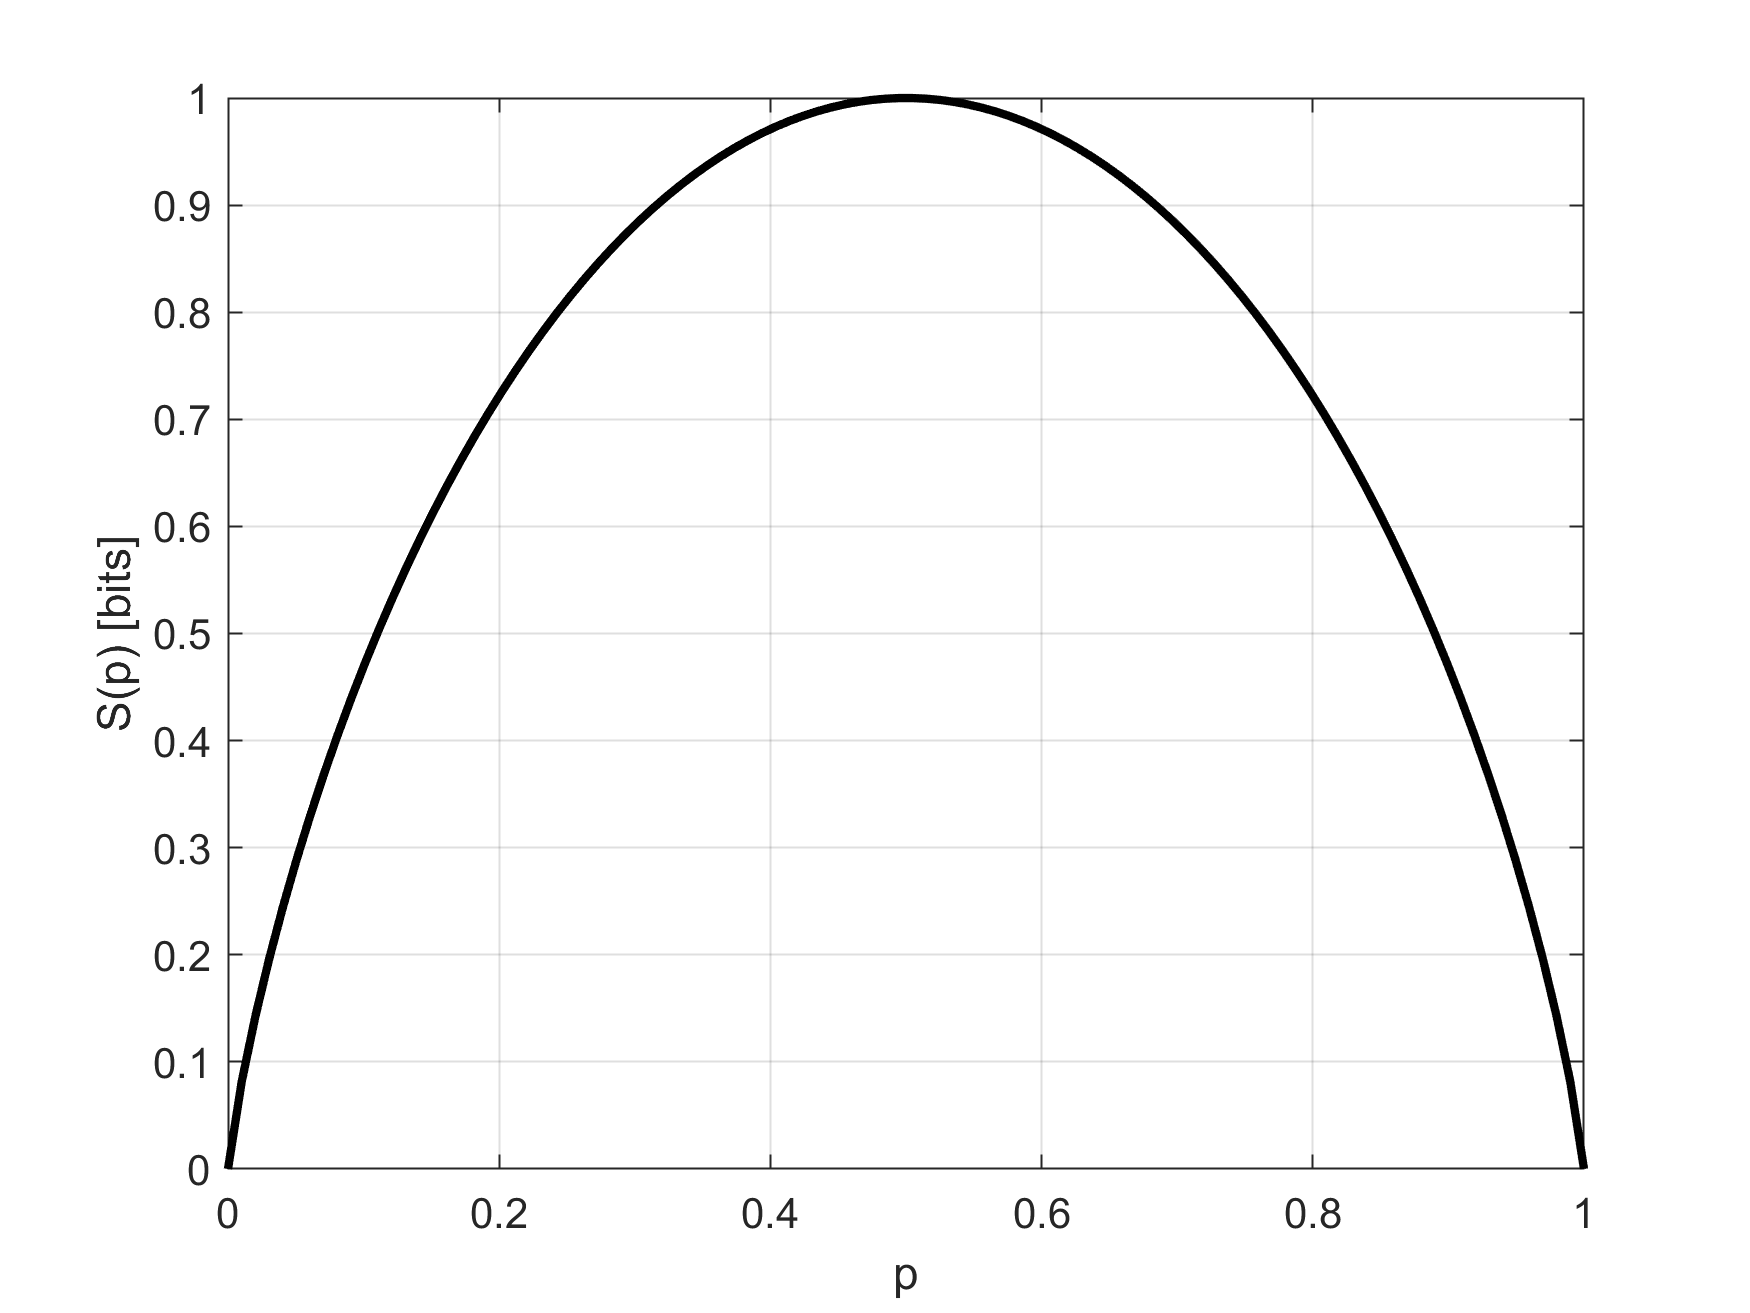
\includegraphics[scale=1]{entropyConc1}
	\end{center}
	\caption{Gráfico de $S(p)$ para un sistema de dos estados.}
	\label{fig-infor2}
\end{figure}
	
Como podemos ver, tenemos el resultado esperado. Para $p=0.5$, es decir, la distribución uniforme, la entropía es máxima e igual a $1 [bit]$, que es el mismo caso del lanzamiento de una moneda. Una interpretación de la entropía es la siguiente: $S(V)$ (donde $V$ es la variable aleatoria) es el número medio de preguntas \textit{binarias}\footnote{En el caso de que la base del logarítmo no sea $2$, ya no son preguntas binarias, por esto la entropía es una función decreciente en la base.} necesarias para poder determinar el valor de la variable. Por ejemplo en el caso del lanzamiento de una moneda el valor de la entropía es $1 [bit]$, debido a que podemos preguntar 'Es cara?', si la respuesta es no, sabremos que es sello. Si la respuesta es si, sabemos que es cara, por lo tanto con una pregunta basta para conocer el estado del sistema.\\
Otro punto importante es que la entropía no depende directamente de los valores que toma la variable aleatoria $V$, sino que depende solo de su distribución (es un funcional de la función de densidad), y como vimos anteriormente corresponde al valor medio de la medida de información. \\
De igual forma que para las densidades de probabilidad definimos las densidades conjuntas y condicionales, podemos definir la entropía conjunta y condicional. La primera está dada por,
\begin{equation*}
	S(V_1,V_2,...,V_n)=-\sum_{V_1} \sum_{V_2}...\sum_{V_n} p(V_1,V_2,...,V_n)\log(p(V_1,V_2,...,V_n))
\end{equation*}
Donde la suma es sobre los valores de las variables aleatorias. La generalización al caso continuo es simplemente, 

\begin{equation*}
	S(V_1,V_2,...,V_n)=-\int_{V_1}\int_{V_2}...\int_{V_n} \rho(V_1,V_2,...,V_n)\log(\rho(V_1,V_2,...,V_n)) dV_1 dV_2...dV_n
\end{equation*}
Vemos que es simplemente una generalización a varias variables, se reemplaza la función de densidad por la función conjunta y se integra sobre todo el espacio de muestra. Ahora para el caso de la entropía conjunta tenemos, 

\begin{align*}
	S(V_1,...,V_s\rvert V_{s+1},...,V_n)&=\langle \log\left(\frac{1}{p(V_1,...,V_s\rvert V_{s+1},...,V_n)}\right) \rangle \\
	&=-\sum_{V_1} \sum_{V_2}...\sum_{V_n} p(V_1,V_2,...,V_n)\log (p(V_1,...,V_s\rvert V_{s+1},...,V_n)) 
\end{align*}
En el caso continuo,

\begin{equation*}
	S(V_1,...,V_s\rvert V_{s+1},...,V_n)=\int_{V_1}...\int_{V_n}\rho(V_1,...,V_n)\log\left(V_1,...,V_s\rvert V_{s+1},...,V_n\right) dV_1 dV_2...dV_n
\end{equation*}
Notemos que esta según esta definición de entropía condicional, $S(V_1,...,V_s\rvert V_{s+1},...,V_n)$ depende de las $n$ variables\footnote{Por ejemplo en el caso de dos variables, es distinto $S(V_1 \rvert V_2)$ que $S(V_1\rvert V_2=v_2)$, la segunda solo depende de la variable $V_1$, mientras que $S(V_1\rvert V_2)$ sería el valor medio de ésta sobre todos los valores de $v_2$, $S(V_1\rvert V_2)=\int_{V_2} \rho(v_2) S(V_1\rvert V_2=v_2) dv_2$.}\\

Una relacion importante entre ambas entropías se obtiene notando que,

\begin{align*}
	\log\left[\rho(V_1)\right] + \log\left[\rho(V_2\rvert V_1)\right]&=log\left[\rho(V_1)\rho(V_2\rvert V_1)\right]\\
	&=\log\left[\rho(V_1)\frac{\rho(V_1,V_2)}{\rho(V_1)}\right]\\
	&=\log\left[\rho(V_1,V_2)\right]
\end{align*}

Donde en la segunda línea se ocupa el teorema de Bayes. Por lo tanto,
\begin{equation*}
	\log\left[\rho(V_1)\right] + \log\left[\rho(V_2\rvert V_1)\right]=\log\left[\rho(V_1,V_2)\right]
\end{equation*}

Entonces, promediando estas variables en ambos lados llegamos a,
\begin{equation*}
	S(V_1,V_2)=S(V_1)+S(V_2\rvert V_1)
\end{equation*}
Esta propiedad es a veces llamada regla de la cadena de la entropía. \\

Ahora vamos a introducir el concepto de entropía relativa, a veces también es llamada \textit{distancia de Kullback-Leibler} (de forma más adecuada llamada \textit{divergencia de Kullback-Leibler}), sin embargo, como observaremos, no es simétrica en sus argumentos por lo que no es una distancia en estricto rigor \footnote{Hay una punto de vista de la teoría de la información desde la geometría diferencial, aunque no profundizaremos en esto aquí, se puede investigar más sobre esto en el libro de Amari \parencite{amari2016}.}. La definición de la entropía relativa es,

\begin{equation*}
	D(\rho,\rho') = \sum_{V_1} p(V_1)\log\left[\frac{p(V_1)}{q(V_1)}\right]
\end{equation*} 

Notemos que la entropía relativa es entre distribuciones, no entre variables aleatorias. Básicamente es una medida de que tan equivocados al asumir una distribución $q$ cuando la distribución real es $p$, en el caso continuo,

\begin{equation*}
	D(p,q) = \int_{V_1} \rho(V_1)\log\left[\frac{\rho(V_1)}{\rho'(V_1)}\right] dV_1 = \langle
 	\log\left[\frac{\rho(V_1)}{\rho'(V_1)}\right]\rangle
\end{equation*} 

Para visualizar ésto podemos estudiar nuevamente el sistema de dos estados, pero ahora consideramos dos probabilidades, $p_1(0)=1-x$, $p_2(1)=x$, $p_2(0)=1-y$, $p_2(1)=y$, por lo tanto la entropía relativa entre ambas distribuciones está dada por,

\begin{equation*}
	D(p_1,p_2)=(1-x)\log\left[\frac{1-x}{1-y}\right]+x\log\left[\frac{x}{y}\right]
\end{equation*}
En la figura \ref{fig-infor3} podemos ver el gráfico de esta función de dos variables. Como es de esperar, la entropía es cero cuando $x=y$, dado que estamos 'asumiendo la distribución correcta' (ambas distribuciones coinciden).

\begin{figure}[H]
	\begin{center}
		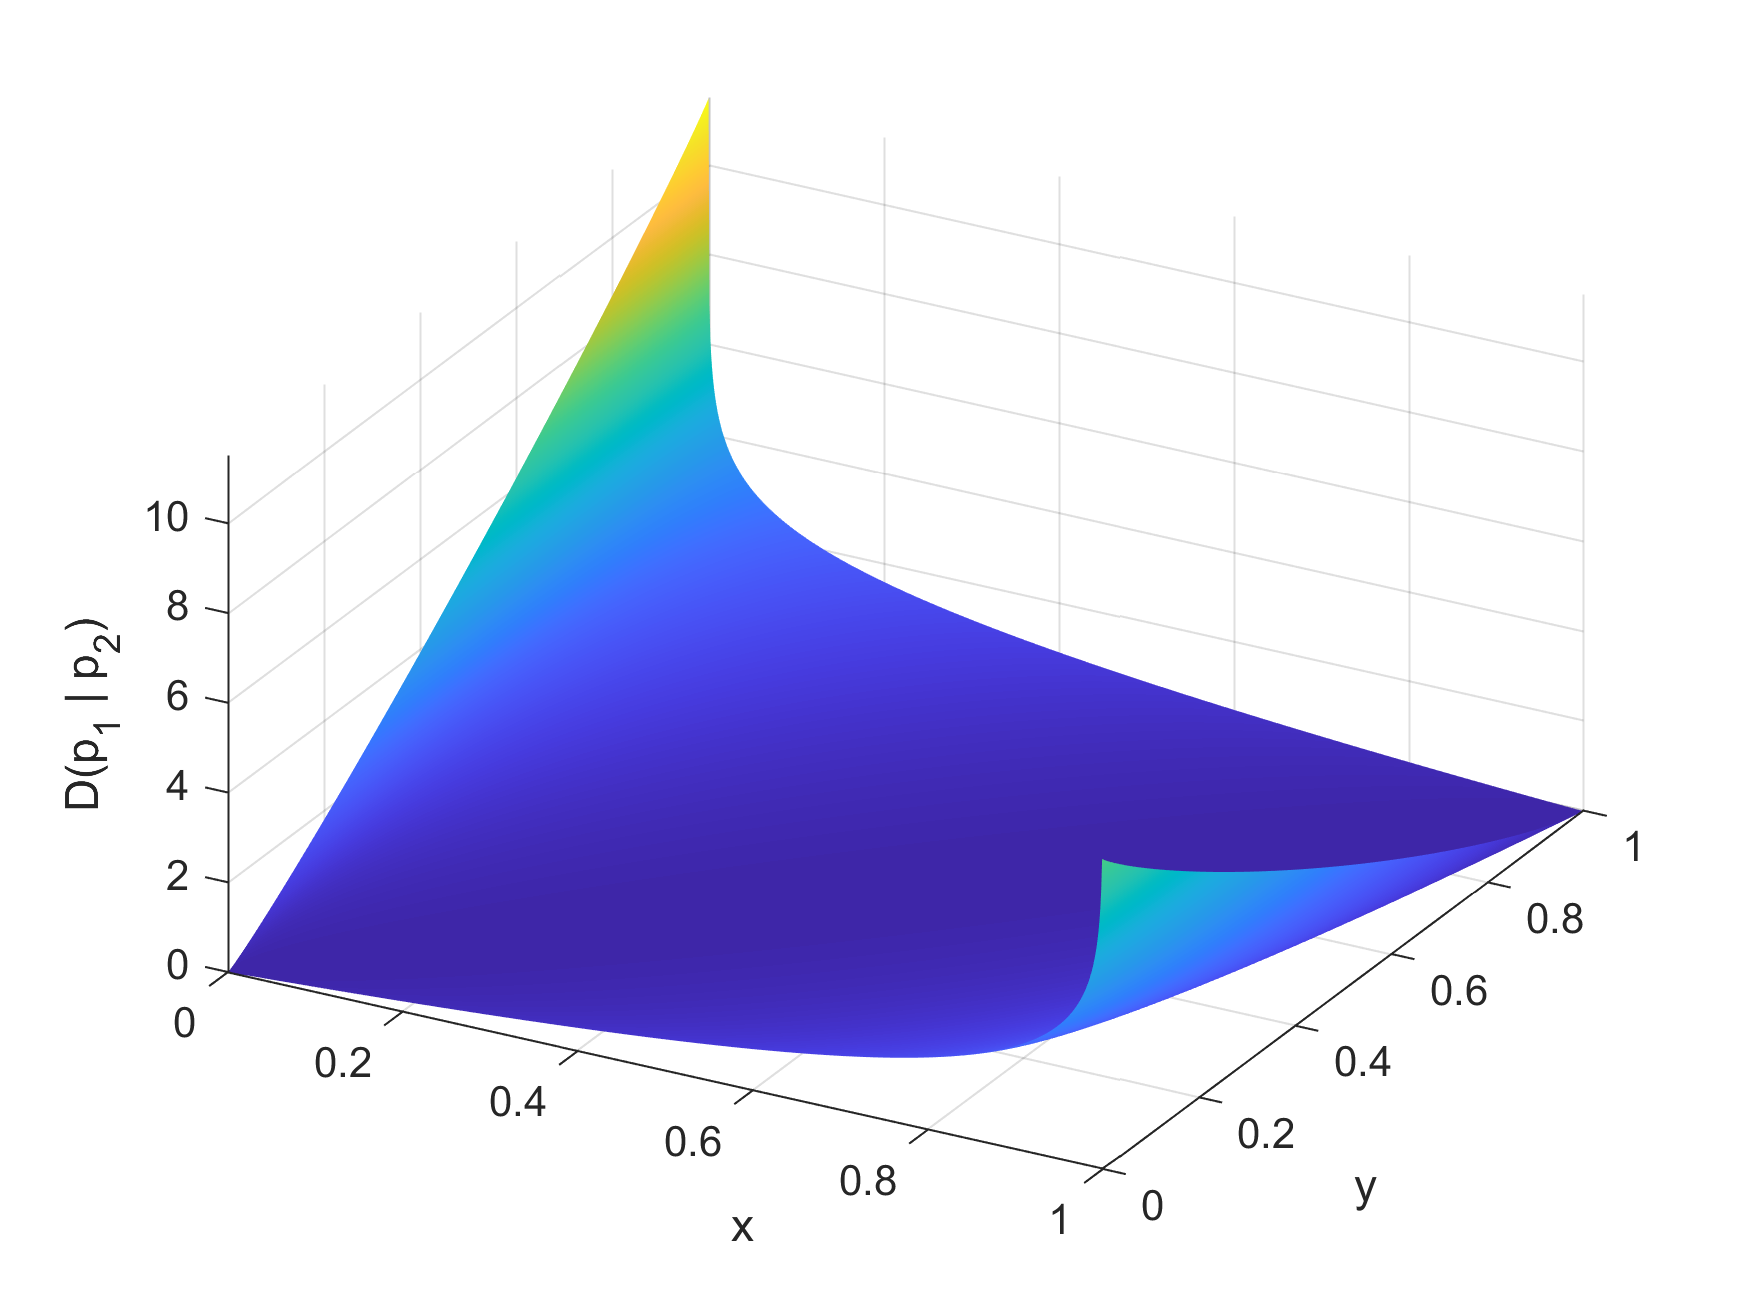
\includegraphics[scale=1]{kullLeib}
	\end{center}
	\caption{Entropía relativa sistema de dos estados.}
	\label{fig-infor3}
\end{figure}



Ahora introduciremos uno de los conceptos más importantes para nuestros propósitos, el de la información mútua. Primero vamos a introducir su definición, dadas dos variables aleatorias $V_1$ y $V_2$, la información mútua entre ambas, $I(V_1,V_2)$ está dada por, 


\begin{equation}
	I(V_1,V_2)=\sum_{V_1}\sum_{V_2} p(V_1,V_2) \log\left[\frac{p(V_1,V_2)}{p(V_1)p(V_2)}\right] =\langle\log\left[\frac{p(V_1,V_2)}{p(V_1)p(V_2)}\right]\rangle
\end{equation} 
En el caso continuo,

\begin{equation}
		I(V_1,V_2)=\int_{V_1}\int_{V_2} \rho(V_1,V_2) \log\left[\frac{\rho(V_1,V_2)}{\rho(V_1)\rho(V_2)}\right]dV_1dV_2
\end{equation}

Una propiedad util de la información mútua es la siguiente, consideremos el logaritmo, 

\begin{align*}
	\log\left[\frac{\rho(V_1,V_2)}{\rho(V_1)\rho(V_2)}\right]&=\log\left[\rho(V_1,V_2)\right]-(\log\left[\rho(V_1)\right] + \log\left[\rho(V_2)\right])\\
	&=S(V_1)+S(V_2)-S(V_1,V_2)\\
	&=S(V_2)-S(V_2\rvert V_1)\\
	&=S(V_1)-S(V_1\rvert V_2)
\end{align*}
Donde las  últimas dos líneas se obtienen a partir de la regla de la cadena para la entropía. Podemos ver claramente que la información mútua es simétrica en sus argumentos, $I(V_1,V_2)=I(V_2,V_1)$, además se observa que $I(V_1,V_1)=S(V_1)$. Si interpretamos $I(V_1,V_2)$ como la reducción en la incertidumbre sobre $V_1$ que nos entrega el conocer $V_1$, entonces podemos ver como la entropía es una medida de información propia de la variable. Una forma visual de entender las cantidades introducidas se muestra en el diagrama de la figura \ref{fig-infor4}.

 
\begin{figure}[H]
	\begin{center}
		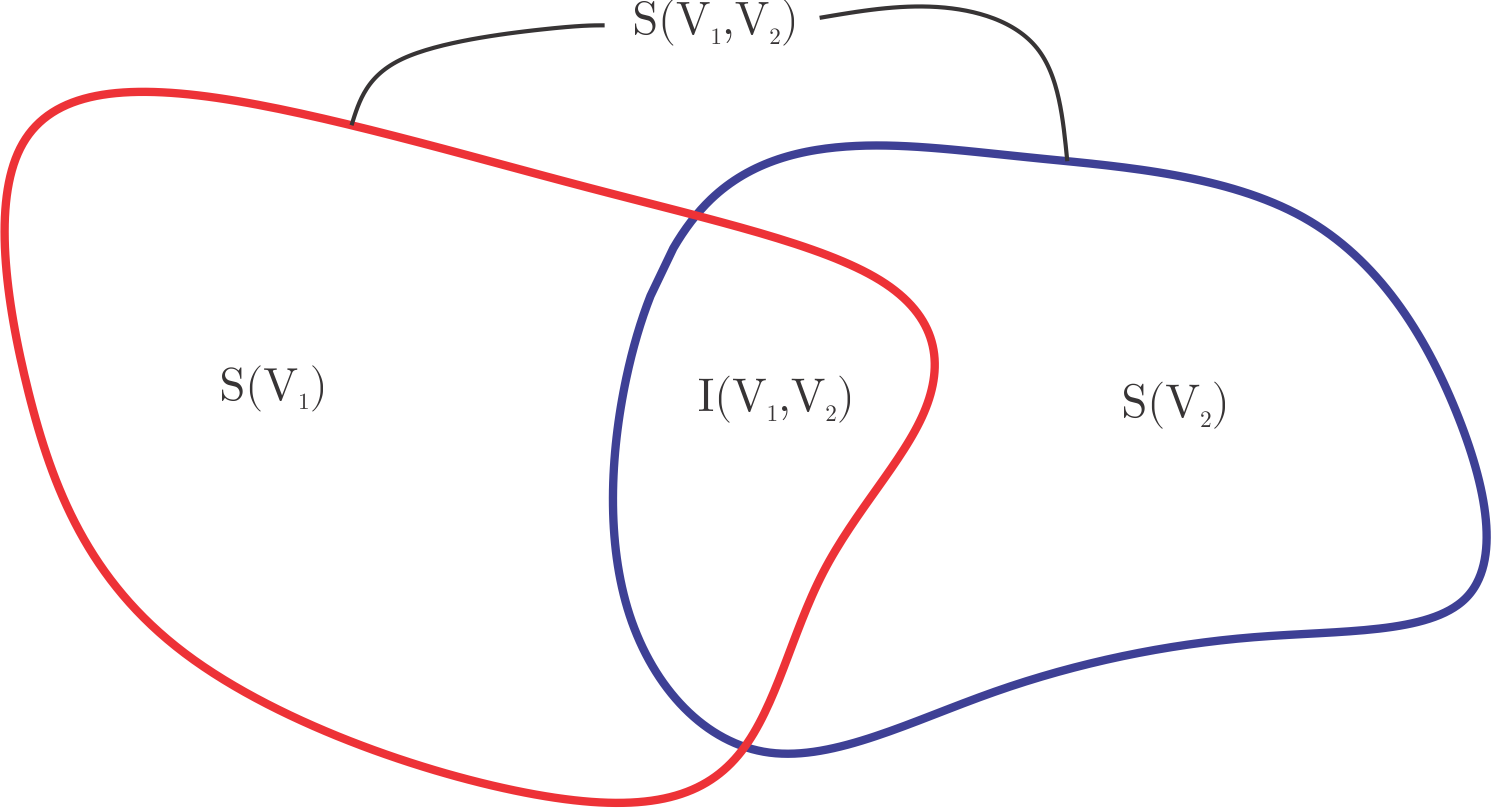
\includegraphics[scale=1]{entropy1}
	\end{center}
	\caption{Diagrama de entropías e información mútua.}
	\label{fig-infor4}
\end{figure}


\subsection{Entropía y física estadística}

A falta de una derivación rigurosa de la mecánica estadística desde el punto de vista de los sistemas dinámicos \parencite{beck2009} (las propiedades de ergodicidad y \textit{mixing} solo se han demostrado para sistemas simples), Jaynes \parencite{jaynes1957} propuso una derivación de la mecánica estadística a partir de la teoría de información. Más precisamente propuso el principio de máxima entropía, que se puede interpretar desde este punto de vista como una minimización de la información (si consideramos que $I=-S$). Esto quiere decir que, bajo ciertas restricciones, asumismo que conocemos lo mínimo posible sobre el sistema (equivalente a decir que eliminamos cualquier tipo de prejuicio o información preconcebida sobre el sistema). Las restricciones pueden ser los valores medios de ciertas cantidades importantes para el sistema, es decir toman la forma,

\begin{equation*}
	\langle C^j \rangle=\sum_i p_i C_i^j
\end{equation*}
donde $i$ es sobre los posibles valores de la cantidad $C^j$, diferentes $j$ indican diferentes cantidades. Luego utilizando el método de los multiplicadores de Lagrange, se busca minimizar la cantidad,

\begin{equation*}
	\Psi [p]= I[p]+\sum_j \beta_j \sum_i p_i C_i ^j
\end{equation*}
Donde $\beta_j$ son los multiplicadores de Lagrange. Derivando con respecto a las probabilidades $p_i$ (con respecto a estas se busca minimizar la información), 

\begin{equation*}
	\pdv{\psi[p]}{p_i}=\pdv{I[p]}{p_i}+\sum_j\beta_jC_i^j=0
\end{equation*}
Otra vez la convexidad de $I$ (o concavidad de $S$) juega un rol importante, dado que para que la ecuación anterior tenga solución única, se debe satisfacer esta propiedad. Cuando consideramos la entropía de Shannon, $I[p]=\sum_i p_i\log(p_i)$, por lo tanto $\pdv{I}{p_i}=1+\log(p_i)$. Luego tenemos,

\begin{equation*}
	1+\log(p_i)+\sum_j\beta_jC_i^j=0\implies p_i=\frac{1}{Z}e^{-\sum_j\beta_j C^j_i }
\end{equation*}
Donde $Z$ es debido a la condición de normalización. Es decir, sabemos que $\sum_i p_i =1$ (esto se puede añadir como otra restricción al problema de optimización). Asumiendo que conocemos los valores medios de diferentes cantidades podemos obtener los distintos ensambles de la mecánica estadística en equilibrio (si asumimos la energía por ejemplo, obtenemos el ensamble canónico). Sin embargo este método no está restringido a sistemas en equilibrio, esto es interesante dado que un cambio en el punto de vista del problema nos permite expandir el método a otros tipos de sistemas.  


\subsection{Otras medidas de información}


La entropía de Shannon no es la única medida de información existente \parencite{beck2009}, a continuación presentamos otras de las más conocidas.\\



\textbf{Entropía de Rényi:} Está definida por,
\begin{equation*}
	S_q^R=\frac{1}{q-1} \log \sum_i p_i^q
\end{equation*}

y contiene la entropía de Shannon como caso especial,

\begin{equation*}
	\lim_{q\to 1} S_q^R=S
\end{equation*}
Un problema de estas entropías es que  su segunda derivada no es siempre positiva, por lo que la concavidad no está asegurada.\\

\textbf{Entropía de Tsallis:} Las entropías de Tsallis también son conocidas como entropías $q$. Están dadas por,

\begin{equation*}
	S_q^T=\frac{1}{q-1}\left(1-\sum p_i ^q\right)
\end{equation*}

y se relacionan con las entropías de Rényi mediante la formula,

\begin{equation*}
	S_q^T=\frac{1}{q-1}\left(1-e^{(q-1)S_q^R}\right)
\end{equation*}
En este caso la entropía si posee concavidad, su segunda derivada está dada por,

\begin{equation*}
	\partial_{p_i} \partial_{p_j} S_q^T=-qp_i^{q-2} \delta_{ij} 
\end{equation*}
Por lo que es concava para $q>0$. A partir de esta entropía se puede derivar la llamada \textit{mecánica estadística no-extensiva}. \\


\textbf{Entropía de Abe:} Es una modificación de la entropía de Tsallis invariante bajo el cambio $q\to q^-1$, está dada por,

\begin{equation*}
	S^A_q=-\sum\frac{p_i^q-p_i^{q^{-1}}}{q-q^{-1}}
\end{equation*}

Y se relaciona con la entropía de Tsallis mediante,

\begin{equation*}
	S_q^{A}=\frac{(q-1)S^T_q-(q^{-1}-1)S^T_{q^{-1}}}{q-q^{-1}}
\end{equation*}
\pagebreak


\section{Estadística y turbulencia}

A continuación aplicaremos las herramientas estadísticas introducidas anteriormente a la turbulencia. Para poder dar una descripción estadística de la turbulencia, descomponemos la velocidad en un valor medio más fluctuaciones,
\begin{equation*}
	\vb{v}=\langle \vb{v}\rangle+\vb{v}'
\end{equation*}
En el estudio de sistemas complejos usualmente se asocian las fluctuaciones a efectos \textit{microscopicos} (en el sentido de que son los efectos de las estructuras más básicas del sistema) y el promedio a efectos \textit{macroscopicos} \parencite{nicolis2012}. El promedio no es el usual definido por una integral, sino que es un promedio de ensamble. Es decir, consideremos que realizamos el mismo experimento $N$ veces, el promedio de los valores en todos los experimentos es el promedio de ensamble,
\begin{equation*}
	\langle v\rangle=\lim_{N\to \infty}\frac{1}{N}\sum_{i=1}^{N}v^{(i)}
\end{equation*}

Este promedio satisface las siguientes propiedades (también llamadas condiciones de Reynolds \parencite{monin1976}),
\begin{align*}
	\langle v+u\rangle=\lim_{N\to \infty}\frac{1}{N}\sum_{i=1}^{N}(u^{(i)}+v^{(i)})=\lim_{N\to \infty}\frac{1}{N}\sum_{i=1}^{N}u^{(i)}+\lim_{N\to \infty}\frac{1}{N}\sum_{i=1}^{N}v^{(i)}=\langle u\rangle+\langle v\rangle
\end{align*}
\begin{equation*}
	\langle av\rangle=\lim_{N\to \infty}\frac{1}{N}\sum_{i=1}^{N}av^{(i)}=a\lim_{N\to \infty}\frac{1}{N}\sum_{i=1}^{N}v^{(i)}=a\langle v\rangle
\end{equation*}
\begin{equation*}
	\langle \partial_j v\rangle=\lim_{N\to \infty}\frac{1}{N}\sum_{i=1}^{N}\partial_jv^{(i)}=\partial_j \lim_{N\to \infty}\frac{1}{N}\sum_{i=1}^{N}v^{(i)}=\partial_j \langle v\rangle
\end{equation*}
\begin{align*}
	\langle \langle v\rangle u\rangle=\langle v\rangle\langle u\rangle 
\end{align*}

Es importante notar que la velocidad media aún puede ser dependiente del tiempo y el espacio, dado que es un promedio sobre un ensamble de experimentos. Como vimos en capitulos anteriores esto se puede escribir en términos de la densidad de probabilidad como,
\begin{equation*}
	\langle v(\vb{x},t) \rangle=\int u \rho(u,\vb{x},t)du
\end{equation*}
Donde la integración es sobre todos los posibles valores de la velocidad. Recordando la función de correlación de dos puntos,
\begin{equation*}
	R_{ij}(\vb{x},\vb{y},t_1,t_2)=\langle u_i(\vb{x},t_1)u_j(\vb{y},t_2)\rangle
\end{equation*}

Ésta función es una medida de como están relacionadas ambas velocidades. Por ejemplo, si fueran señales oscilantes y estuvieran completamente en fase, el producto $u_i$ con $u_j$ sería siempre positivo y se tendría un valor alto para la correlación. Esta función se puede expresar convenientemente en términos del punto medio, $\vb{R}=\frac{\vb{x}+\vb{y}}{2}$ y la diferencia entre ambos puntos $\vb{r}=\vb{x}-\vb{y}$ (lo mismo para los tiempos, el tiempo medio $T$ y la diferencia de tiempo $\tau$),
\begin{equation*}
	R_{ij}(\vb{x},\vb{y},t_1,t_2)=R_{ij}(\vb{R},\vb{r},T,\tau)
\end{equation*}
Una ventaja de expresar la correlación en términos de estas variables es que, en el caso de turbulencia homogénea y estacionaria, la función solo dependerá de la diferencia de tiempo $\tau$ y la diferencia de posición $\vb{r}$ por lo tanto en este caso tenemos,
\begin{equation*}
	R_{ij}(\vb{r},\tau)=\langle u_i(\vb{x},t_1)u_j(\vb{x}+\vb{r},t_2)\rangle
\end{equation*}
Dado que estas funciones dependen de la posición y el tiempo, una pregunta fundamental es: A que distancia (y tiempo) las señales pierden su correlación? Estas escalas son llamadas escalas integrales, de tiempo y espacio, como fueron definidas anteriormente. \\
Si se reescribe la función de correlación como (según lo indicado por McComb \parencite{mccomb1990}),
\begin{equation*}
	R_{ij}(\vb{x},\vb{y},t_1,t_2)=Q_{ij}(\vb{x},\vb{y},t_1,t_2)\langle v_i(\vb{x},t_1)\rangle_{rms}\langle v_j(\vb{y},t_2)\rangle_{rms}
\end{equation*}
Donde  $Q_{ij}$ es llamado el coeficiente de correlación y los promedios de las velocidades son RMS. Este coeficiente debe satisfacer,
\begin{equation*}
	Q_{ij}\to 0 \hspace{0.25cm} \text{si}\hspace{0.25cm} \abs{\vb{x}-\vb{y}}\to\infty 
\end{equation*} 
\begin{equation*}
Q_{ij}\to 0 \hspace{0.25cm} \text{si}\hspace{0.25cm} \abs{t_1-t_2}\to\infty 
\end{equation*}
Es decir, que las velocidades pierdan su correlación a grandes distancias temporales y espaciales. Entonces, fijando $\vb{x}=\vb{y}=\vb{0}$ y $T=0$, se define la escala de tiempo integral como,
\begin{equation*}
	T_I=\int_0^\infty Q(\tau)d\tau
\end{equation*} 
Donde $Q$ es alguna componente del coeficiente de correlación. El valor de esta escala debería ser el mismo para todas las componentes. También definimos una escala integral espacial (fijando $t_1=t_2=0$ y $\vb{R}=\vb{0}$) como,
\begin{equation*}
	L_{ij}(\hat{\vb{r}})=\int_0^\infty Q_{ij}(\vb{r})d\abs{\vb{r}}
\end{equation*} 
Ésta escala depende, en general, tanto de las componentes que se comparen como de la dirección.\\



\begin{figure}[H]
	\begin{center}
		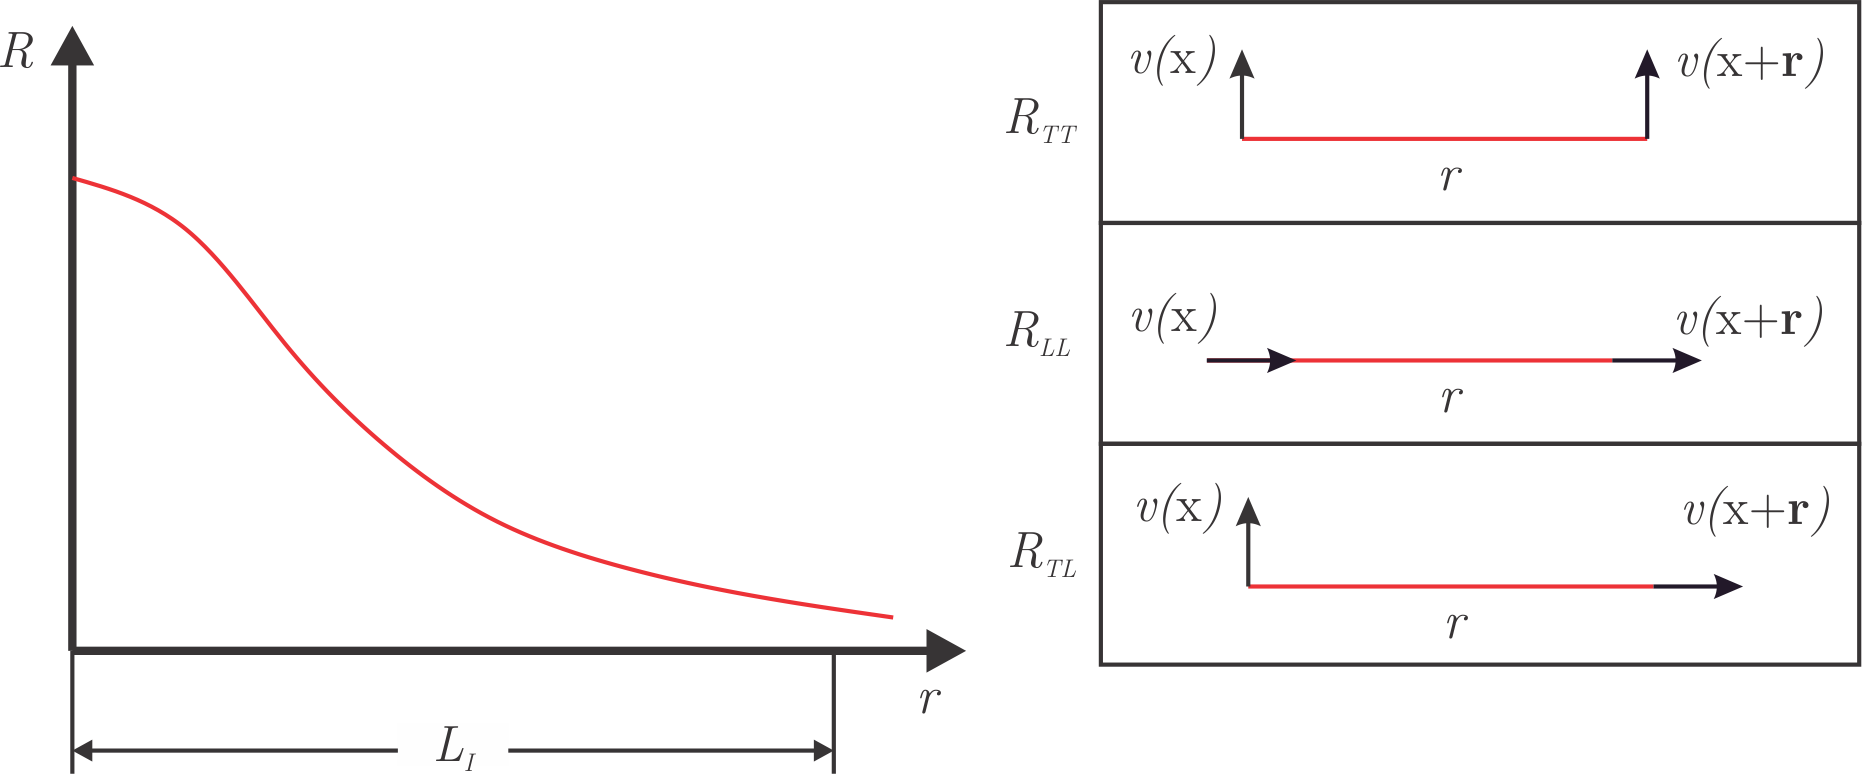
\includegraphics[scale=0.9]{correlationLength}
	\end{center}
	\caption{Esquema de longitud de correlación (izquierda) y componentes del tensor de correlación (derecha).}
	\label{fig-correl}
\end{figure}

El tensor de correlación entonces se puede dividir en partes longitudinales, transversales o cruzadas como se muestra en la figura \ref{fig-correl}. Estas funciones se pueden relacionar con la energía cinética, recordemos que,
\begin{equation}
	E= \frac{1}{2}\langle u_iu_i \rangle = \frac{1}{2}R_{ii}(0)
	\label{eq.ener1}
\end{equation}
Donde el tensor está evaluado en $0$ dado que solo depende de la diferencia de los puntos. \\
Ahora, para el caso isótropo debe haber invarianza bajo rotaciones y reflexiones. La primera implica las siguientes propiedades del tensor de correlación de un punto \parencite{mccomb1990},

\begin{equation*}
	\langle v_1^2\rangle=\langle v_2^2\rangle=\langle v_3^2\rangle=\langle v^2\rangle
\end{equation*} 
Mientras que de la simetría bajo reflexiones se tiene,
\begin{equation*}
	\langle v_1v_2\rangle=\langle v_2v_3\rangle=\langle v_1v_3\rangle=0
\end{equation*}
Por lo tanto ahora podemos escribir la energía (\ref{eq.ener1}) como,

\begin{equation*}
	E=\frac{1}{2}R_{ii}(0)=\frac{1}{2}\left(\langle v_1^2\rangle+\langle v_2^2\rangle+\langle v_3^2\rangle\right)=\frac{3}{2}\langle v^2\rangle \label{eq.ener2}
\end{equation*}

Ahora considerando el tensor de correlación en el caso isótropo pero de dos puntos, éste se `puede escribir como \parencite{landau1959,mccomb1990}, 

\begin{equation}
	R_{ij}(\vb{r})=A(r)\hat{n}_i\hat{n}_j+B(r)\delta_{ij}
\end{equation}
Donde $\hat{n}$ es un vector unitario en la dirección de $\vb{r}$. Ahora, es más útil expresar las expresiones en términos de las componentes transversales y longitudinales (como son definidas en la figura \ref{fig-correl}). Los coeficientes de correlación longitudinal ($f(r)$) y transversal ($g(r)$) son definidos tales que,
\begin{equation*}
	\langle v^2 \rangle f(r)=\langle v_L(\vb{x})v_L(\vb{x}+\vb{r}) \rangle\hspace{0.5cm} \langle v^2 \rangle g(r)=\langle v_T(\vb{x})v_T(\vb{x}+\vb{r})\rangle
\end{equation*}

Ahora, como relacionamos éstas componentes con los coeficientes $A(r)$ y $B(r)$? Para eso consideremos un caso particular en el que el vector $\vb{r}$ está sobre un eje coordenado, por ejemplo x. Entonces tendremos que la componente $R_{11}$ estará dada por,
\begin{equation*}
	R_{11}=A(r)+B(r)
\end{equation*}
Pero además sabemos que ésta coincide con las componentes longitudinales de la velocidad, por lo que tenemos,
\begin{equation*}
	A(r)+B(r)=\langle v^2 \rangle f(r)
\end{equation*}
De la misma forma, si consideramos $R_{22}$, los vectores unitarios tienen componente cero en ésta dirección, que corresponde a la transversal por lo que tenemos,
\begin{equation*}
	R_{22}=B(r)=\langle v^2 \rangle g(r)
\end{equation*}
Ésto nos permite escribir el tensor de correlación como,
\begin{equation}
	R_{ij}=\langle v^2 \rangle g(r) \delta_{ij}+\langle v^2 \rangle(f(r)- g(r))n_in_j
	\label{eq-corr2}
\end{equation}
Ahora, recordemos que el tensor de correlación en su forma más general está dado por,
\begin{equation*}
	R_{ij}(\vb{r})=\langle v_i(\vb{x})v_j(\vb{x}') \rangle
\end{equation*}
Entonces si derivamos con respecto a $x_i$ tendremos \parencite{karman1938},
\begin{equation*}
	\partial_{i} R_{ij}=\langle \partial_i v_i(\vb{x})v_j(\vb{x}') \rangle=0
\end{equation*}
Donde se aplica la condición de incompresibilidad. Ahora podemos usar esto para relacionar las funciones $f$ y $g$ derivando el tensor de correlación con respecto a $r_{i}$ (considerando que $n_i=r_i/r$),
\begin{equation*}
	\partial_{i} R_{ij}=\langle v^2 \rangle\partial_i\left[ g(r) \delta_{ij}+(f(r)- g(r))\frac{r_i r_j}{r^2}\right]=0
\end{equation*}
Es útil tener en cuenta al siguiente relación para la derivada de $r$ con respecto a la componente $r_i$,
\begin{equation*}
	\partial_i r^n = n r^{n-2}r_i
\end{equation*}
Ahora para la segunda parte tenemos,
\begin{align*}
	\partial\left[(f(r)- g(r))\frac{r_i r_j}{r^2}\right]&=\frac{r_ir_j}{r^2}\partial_i(f-g)+(f-g)\partial_i\left(\frac{r_ir_j}{r^2}\right)\\
	&=(f'-g')\partial_ir\frac{r_i r_j}{r^2}+(f-g)\left[\frac{\partial_i(r_ir_j)}{r^2}+r_ir_j\partial_i(r^{-2})\right]\\
	&=(f'-g')r^{-1}r_i\frac{r_i r_j}{r^2}+(f-g)\left[\frac{r_j\partial_i r_i+r_i\partial_ir_j}{r^2}+r_ir_j\frac{(-2r_i)}{r^4}\right]\\
	&=(f'-g')\frac{(r_ir_i) r_j}{r^3}+(f-g)\left[\frac{3r_j+r_i\delta_{ij}}{r^2}-2\frac{r_j(r_ir_i)}{r^4}\right]\\
	&=(f'-g')\frac{r^2 r_j}{r^3}+(f-g)\left[\frac{4r_j}{r^2}-2\frac{r_jr^2}{r^4}\right]\\
	&=(f'-g')\frac{ r_j}{r}+\frac{(f-g)}{r^2}(2r_j)\\
	&=(f'-g')\frac{ r_j}{r}+2r_j\frac{(f-g)}{r^2}
\end{align*}
Mientras que para la otra parte de la derivada del tensor se tiene,
\begin{equation*}
	\partial_i(g\delta_{ij})=g'r^{-1}r_i\delta_{ij}=\frac{g'}{r}r_j
\end{equation*}
Por lo tanto reemplazando llegamos a,
\begin{equation*}
	\partial_{i} R_{ij}=\langle v^2 \rangle \frac{r_j}{r}\left[g'+(f'-g') +2\frac{(f-g)}{r}\right]=0
\end{equation*}
Entonces para que esto se cumpla en general,
\begin{equation*}
	g'+(f'-g') +2\frac{(f-g)}{r}=0\implies g=\frac{r}{2}f'+f 
\end{equation*}
Y reemplazando podemos expresar todo el tensor de correlacion de dos puntos (isótropo) solo en términos de la función $f(r)$,
\begin{equation}
	R_{ij}(\vb{r})=\langle v^2 \rangle f(r) \delta_{ij}+\frac{1}{2}f'(r)\left(\delta_{ij}-n_in_j\right) \label{eq.corr2}
\end{equation}
Es importante notar que la funcion $f$, también se puede denotar por $f_{2,L}(r)$ corresponde a la parte longitudinal del tensor de correlación. Siguiendo un procedimiento similar se puede obtener la siguiente relación para el tensor de correlación de tercer orden en términos de su función longitudinal $f_{3,L}(r)$ \parencite{friedrich2020},

\begin{equation}
	R_{ij,k}(r)=-\frac{r^2}{2}\partial_r\left[\frac{f_{3,L}(r)}{r}\right]n_in_jn_k+\frac{1}{4r}\partial_{r}\left[f_{3,L}(r)\right]\left[n_i\delta_{jk}+n_j\delta_{ik}\right]
	-\frac{f_{3,L}(r)}{2}n_k\delta_{ij}
	\label{eq.corr3}
\end{equation}
Otra herramienta útil utilizada en la teoría estadística de la turbulencia son las llamadas funciones de estructura. Éstas están definidas como,
\begin{equation*}
	S_n(\vb{r})=\langle \left[v(\vb{x+r})-v(\vb{x})\right]^n\rangle
\end{equation*}
En particular, para el caso homogéneo e isótropo se tiene, 
\begin{equation*}
	S_n(r)=\langle \left[v(r)-v(0)\right]^n\rangle
\end{equation*}
Observamos que ya no existe dependencia en el vector de posición, sino en su magnitud (por la isotropía). Además, su relación con el coeficiente de correlación longitudinal, el cual podemos llamar $Q_{LL}(r)=f(r)$ es (para la función de estructura de segundo orden),
\begin{equation*}
	S_2(r)=2\langle v^2 \rangle(1-f(r))
\end{equation*}


\pagebreak 


\section{Las ecuaciones de Navier-Stokes}

Éstas son las ecuaciones que describen la turbulencia hidrodinámica, y en los fluidos es donde primero se observó el fenómeno de la turbulencia, las ecuaciones en sí son (para el caso de un fluido incompresible),

\begin{equation}
	\partial_t \vb{v}+\underbrace{(\vb{v}\cdot\vb{\grad{}})\vb{v}}_{\text{No linealidad}}=-\frac{1}{\rho}\vb{\grad{}}p+\underbrace{\nu^2\laplacian{}\vb{v}}_{\text{Disipación}}
\label{eq.NS}
\end{equation}
 Algunos, como Uriel Frisch \parencite{frisch1995}, creen que éstas ecuaciones contienen toda la turbulencia. Sin embargo otros autores como Zakharov, Falkovich o Cardy \parencite{cardy2008} argumentan que el fenómeno de la turbulencia es mucho más amplio que la turbulencia hidrodinámica.  


\subsection{Ecuaciones de Navier-Stokes en forma solenoidal}

Lo primero que buscamos es expresar las ecuaciones de N-S solo en términos de la velocidad. Para esto primero recordamos que en el caso de un fluido incompresible tenemos,
\begin{equation*}
	\vb{\grad{}}\cdot\vb{v}=0
\end{equation*}
Entonces, tomando la divergencia de la ecuación \ref{eq.NS}m para el lado izquierdo tenemos (ahora trabajamos en notación indicial, donde índices repetidos implican una suma),
\begin{align*}
	\partial_i \left[\partial_t v_i+(v_j\partial_j)v_i\right]&=\cancelto{0}{\partial_t \partial_i v_i}+\partial_i\left[(v_j\partial_j)v_i\right]\\
	&=\partial_i(v_j\partial_j)v_i+\cancelto{0}{(v_j\partial_j)(\partial_iv_i)}\\
	&=(\partial_iv_j)(\partial_j v_i)+v_j\partial_i\partial_jv_i\\
	&=(\partial_iv_j)(\partial_j v_i)+\cancelto{0}{v_j\partial_j \partial_iv_i}\\
	&=(\partial_i v_j)(\partial_j v_i)
\end{align*}

Donde se utiliza la condición de incompresibilidad para anular los términos, entre la tercera y cuarta línea se usa la conmutatividad de las derivadas parciales. Ahora consideremos el término $\partial_i\partial_j(v_iv_j)$, si lo desarrollamos tenemos,
\begin{align*}
	\partial_i\partial_j(v_iv_j)&=\partial_i \left[(\partial_j v_i)v_j+v_i(\partial_j v_j)\right]\\
	&=\partial_i(v_j \partial_j v_i)\\
	&=\partial_i v_j \partial_j v_i + v_j \partial _j \partial_i v_i\\
	&=(\partial_i v_j)(\partial_j v_i)
\end{align*}
Por lo tanto, al tomar la divergencia de la ecuación de N-S el lado izquierdo se puede escribir como,
\begin{equation*}
		\partial_i \left[\partial_t v_i+(v_j\partial_j)v_i\right]=\partial_i\partial_j (v_iv_j)
\end{equation*}
En el lado derecho se anula el término asociado a la disipación por la conmutatividad de las derivadas parciales. Entonces llegamos a la siguiente ecuación para la presión en términos de la velocidad,
\begin{equation}
	\frac{1}{\rho}\partial_i\partial_i p=-\partial_i\partial_j (v_iv_j) \label{eq.Pres}
\end{equation}

Ahora introduciremos el concepto de función de Green, éstas son funciones $G(\vb{x},\vb{x}')$ tales que, dado un operador diferencial $\hat{L}_{\vb{x}}$ cumplen la relación,
\begin{equation*}
	\hat{L}_{\vb{x}}G(\vb{x},\vb{x}')=\delta(\vb{x}-\vb{x}')
\end{equation*}
Ésta ecuación se resuelve sujeta a las mismas condiciones de borde del problema que queremos solucionar, el cual está dado por,
\begin{equation*}
	\hat{L}_{\vb{x}} p =f(\vb{x})
\end{equation*}
Entonces, la solución estará dada por,
\begin{equation*}
	p(\vb{x})=\int G(\vb{x},\vb{x}')f(\vb{x}')d\vb{x}'
\end{equation*}

Es simple ver que, de hecho, ésta solución satisface la ecuación original. Simplemente operamos el operador $\hat{L}_{\vb{x}}$ en ambos lados,
\begin{align*}
	\hat{L}_{\vb{x}}&=\hat{L}_{\vb{x}}\left(\int G(\vb{x},\vb{x}')f(\vb{x}')d\vb{x}'\right)\\
	&=\int \hat{L}_{\vb{x}}G(\vb{x},\vb{x}')f(\vb{x}')d\vb{x}'\\
	&=\int \delta(\vb{x}-\vb{x}')f(\vb{x}')d\vb{x}'\\
	&=f(\vb{x})
\end{align*}
Donde entre la tercera y cuarta línea utilizamos la definición de función de Green y entre la cuarta y quinta línea utilizamos la propiedad principal de la función Delta de Dirac. \\
En este caso, se utiliza la siguiente ecuación de borde para las ecuaciones de N-S \parencite{mccomb1990},
\begin{equation*}
	v_i(\vb{x})=0\hspace{0.25cm}\text{si}\hspace{0.25cm} \vb{x}\in S 
\end{equation*}

Donde $S$ es el contorno del volumen en el cual solucionamos las ecuaciones. Por lo tanto, al considerar las ecuaciones sobre este contorno, se anulan los términos $\partial_t v_i$ (debido a que la condición de borde es válida para cualquier tiempo $t$) y $(v_i\partial_i)$, entonces quedamos con,
\begin{equation}
	\frac{1}{\rho}\partial_i p=\nu\partial_j \partial_j v_i \label{eq.BC}
\end{equation}
Donde el término del Laplaciano no se anula, dado que las derivadas de la velocidad no tienen por que ser nulas en el contorno. Ahora podemos expresar ésta condición en términos de las derivadas normales a la superficie,
\begin{equation*}
	\partial^2_n=n_{m}n_n\partial_n\partial_m
\end{equation*}
Si tomamos el producto escalar de la condición \ref{eq.BC} con la normal $n_i$ se tiene,
\begin{equation}
	\frac{1}{\rho}\partial_n p =\nu n_i \partial_j\partial_j v_i
\end{equation}
Y si ahora tomamos el producto punto 2 veces con $n_j$, considerando que $n_j n_j=1$ dado que es un vector unitario,
\begin{equation*}
	\frac{1}{\rho}\partial_n p =\nu n_i (n_j\partial_j)(n_j\partial_j)v_i
\end{equation*}
Entonces podemos escribir la condición de borde en términos de derivadas normales a $S$ como,
\begin{equation*}
	\frac{1}{\rho}\partial_n p=n_i \nu \partial_n^2v_i
\end{equation*}
Y para la función de Green,
\begin{equation*}
	\partial_n G(\vb{x},\vb{x}')=0\hspace{0.25cm} \text{si}\hspace{0.25cm} \vb{x}\in S
\end{equation*}
Y la solución para la presión se puede expresar entonces como,
\begin{equation*}
	P(\vb{x})=\rho\partial_i\partial_j\int_V G(\vb{x},\vb{x}')v_i(\vb{x}')v_j(\vb{x}')d\vb{x}'+\nu\rho\int_S G(\vb{x},\vb{x}')n_i\partial^2_nv_i(\vb{x}') d\vb{x}'
\end{equation*}
Notar que la primera integral es sobre el volumen, mientras que la segunda sobre $S$ (éste término proviene de la condición de borde).
Si ahora definimos los siguientes operadores,
\begin{align*}
	\hat{D}_{mn}(\cdot)&=\delta_{mn}(\cdot)-\partial_m\partial_n\int_V G(\vb{x},\vb{x}')(\cdot)d\vb{x}'\\
	\hat{L}_{mn}(\cdot)&=\nu\partial_m\int_S G(\vb{x},\vb{x}')n_n\partial^2_n(\cdot)d\vb{x}'
\end{align*}
Donde el punto indica que estos operadores pueden actuar sobre cualquier función. Ahora si definimos el operador $\hat{M}_{mnl}(\cdot)$ como,
\begin{equation*}
	\hat{M}_{mnl}(\cdot)=-\frac{1}{2}\left[\partial_n\hat{D}_{ml}(\cdot)+\partial_l\hat{D}_{mn}(\cdot)\right]
\end{equation*}

Con lo cual finalmente podemos escribir la ecuación de N-S como,
\begin{equation}
	\left(\partial_t-\nu\laplacian{}\right)v_i(\vb{x},t)=\hat{M}_{imn}\left(v_m(\vb{x,t})v_n(\vb{x},t)\right)-\hat{L}_{im}(u_m(\vb{x},t))
\end{equation}

\subsection{Ecuaciones de Navier-Stokes en espacio de Fourier}

Ahora centramos nuestra atención a transformar las ecuaciones de N-S de un espacio en $\vb{x}$ a un espacio en $\vb{k}$, notar que la transformada de Fourier es sobre las coordenadas espaciales y no las temporales. Primero consideremos el caso de una caja finita con condiciones de borde periódicas, de ésta forma la variable $\vb{k}$ tomará valores discretos. La transformada inversa de la velocidad en este caso es,
\begin{equation*}
	v_i(\vb{x},t)=\frac{1}{\sqrt{V}}\sum_{\vb{k}}e^{i\vb{k}\cdot\vb{x}}v_i(\vb{k},t)
\end{equation*}
Y la transformada directa es,
\begin{equation*}
	v_i(\vb{k},t)=v_{i,\vb{k}}(t)=\frac{1}{\sqrt{V}}\int e^{i\vb{k}\cdot\vb{x}} v_i(\vb{x},t)d\vb{x}
\end{equation*}
Para poder realizar la transformada de las ecuaciones necesitamos la siguiente herramienta (teorema de convolución), consideremos dos funciones $f(t)$ y $g(t)$, su producto entonces es,
\begin{equation*}
	w(t)=f(t)g(t)
\end{equation*}
Ahora tenemos,
\begin{equation*}
	f(t)=\int f(k)e^{ikt}dk \hspace{0.5cm} g(t)=\int g(q)e^{iqt}dq
\end{equation*}
Luego reemplazando llegamos a,
\begin{align*}
	w(t)&=f(t)g(t)\\
	&=\int f(k)e^{ikt}dk\int g(q)e^{iqt}dq\\
	&=\int f(k)g(q)e^{i(k+q)t}dk dq\\
\end{align*}
Aquí es donde se realiza el cambio $q=j-k$, por lo tanto llegamos a,
\begin{equation*}
	w(t)=\int f(k)g(j-k)e^{i j t}dk dj=\int w(j) e^{i j t} dj
\end{equation*}
Donde $w(j)$ es la transformada de Fourier del producto $w(t)$. Ahora, considerando término por término las ecuaciones de N-S tenemos, para la derivada temporal se tiene,
\begin{equation*}
	\partial_tv_i(\vb{x},t)=\sum_{\vb{k}}\partial_tv_{i,\vb{k}}e^{i\vb{k}\cdot\vb{x}}
\end{equation*}
Para la parte no lineal, usando la convolución mostrada anteriormente,
\begin{align*}
	v_j\partial_jv_i&=\left(\sum_{\vb{q}}v_{j,\vb{q}}e^{i\vb{q}\cdot\vb{x}}\right)\partial_j\left(\sum_{\vb{k}}v_{i,\vb{k}}e^{i\vb{k}\cdot\vb{x}}\right)\\
	&=i\sum_{\vb{k}}k_j \sum_{\vb{q}}v_{j,\vb{q}}v_{i,\vb{k}}e^{i(\vb{q}+\vb{k})\cdot\vb{x}}
\end{align*}
Ahora, con el teorema de convolución llegamos a,
\begin{equation*}
	i\sum_{\vb{k}}k_j \sum_{\vb{q}}v_{j,\vb{q}}v_{i,\vb{k}}e^{i(\vb{q}+\vb{k})\cdot\vb{x}}=\sum_{\vb{k}} i k_j \sum_{\vb{j}}v_{j,\vb{k}-\vb{j}}v_{i,\vb{j}}e^{i\vb{k}\cdot\vb{x}}
\end{equation*}

Ahora, recordando la ecuación para la presión \ref{eq.Pres}, notando que (transformando la presión en forma similar a la velocidad)

\begin{equation*}
	\partial_i^2 p(\vb{x},t)=-k^2\sum_{\vb{k}} p_{\vb{k}}e^{i\vb{k}\cdot\vb{x}}
\end{equation*}
Mientras que para el lado derecho de \ref{eq.Pres}, aplicando el teorema de convolución llegamos a,
\begin{equation*}
	\partial_i\partial_j(v_i(\vb{x},t)v_j(\vb{x,t}))=-\sum_{\vb{k}} k_i k_j \sum_{\vb{j}}v_{i,\vb{k-j}}v_{j,\vb{j}} e^{i\vb{k\cdot\vb{x}}}
\end{equation*} 
Por lo que la transformada de la ecuación queda,
\begin{equation*}
	p(\vb{k})=-\frac{k_ik_j}{k^2}\sum_{\vb{j}}v_{i,\vb{k-j}}v_{j,\vb{j}}
\end{equation*}
Para el término viscoso tendremos,
\begin{equation*}
	\nu \partial_j ^2 v_{i}(\vb{x},t)=-k^2\nu\sum_{\vb{k}}v_{i,\vb{k}} e^{i\vb{k}\cdot\vb{x}}
\end{equation*}
Donde el signo negativo proviene de la multiplicación $(ik_j)(ik_j)$, donde $i=\sqrt{-1}$. Y para la presión, en la ecuación de N-S,
\begin{equation*}
	\partial_i p(\vb{x},t)=\sum_{\vb{k}}k_ip_{\vb{k}}e^{i\vb{k}\cdot\vb{x}}
\end{equation*}
Finalmente, reemplazando en la ecuación llegamos a la siguiente forma,
\begin{equation*}
	\left(\partial_t +\nu k^2\right)v_{i,\vb{k}}=-ik_ip_{\vb{k}}-ik_j\sum_{\vb{j}}v_{i,\vb{j}-\vb{k}}v_{j,\vb{k}}
\end{equation*}

Y reemplazando la expresión obtenida para $p_{\vb{k}}=p(\vb{k})$,
\begin{align*}
	\left(\partial_t +\nu k^2\right)v_{i,\vb{k}}&=i\frac{k_ik_jk_l}{k^2}\sum_{\vb{j}}v_{j,\vb{k-j}}v_{l,\vb{j}}-ik_j\sum_{\vb{j}}v_{i,\vb{k}-\vb{j}}v_{j,\vb{k}}\\
	&=-ik_i\left[-\frac{k_mk_n}{k^2}\sum_{\vb{j}}v_{m,\vb{k-j}}v_{n,\vb{j}}+\delta_{mn}\sum_{\vb{j}}v_{m,\vb{j}+\vb{k}}v_{n,\vb{j}}\right]\\
	&=-ik_i\left[\delta_{mn}-\frac{k_mk_n}{k^2}\right]\sum_{\vb{j}}v_{m,\vb{k}-\vb{j}}v_{n,\vb{j}}\\
	&=-ik_iP_{mn}\sum_{\vb{j}}v_{m,\vb{j}+\vb{k}}v_{n,\vb{k}}\\
	&=N_{imn}(\vb{k})\sum_{\vb{j}}v_{m,\vb{j}+\vb{k}}v_{n,\vb{k}}
\end{align*}
Por lo tanto finalmente la ecuación de Navier-Stokes en el espacio de Fourier toma la forma,
\begin{equation}
\left(\partial_t +\nu k^2\right)v_{i,\vb{k}}=	N_{imn}(\vb{k})\sum_{\vb{j}}v_{m,\vb{j}+\vb{k}}v_{n,\vb{k}} \label{eq.NSF}
\end{equation}

Ésta ecuación puede ser simetrizada simplemente introduciendo el operador simétrico,
\begin{equation*}
	\hat{M}_{imn}(\vb{k})=\frac{1}{2}\left[N_{imn}(\vb{k})+N_{inm}(\vb{k})\right]
\end{equation*}
Y reemplazando en la ecuación por $N_{imn}(\vb{k})$.\\
También es importante la ecuación de continuidad en el espacio de Fourier, recordemos que la velocidad puede escribirse (en el caso continuo) como,
\begin{equation*}
	v_i(\vb{x},t)=\frac{1}{\sqrt{V}}\int e^{i\vb{k}\cdot\vb{x}}v_i(\vb{k},t)d^3k
\end{equation*}
De la condición de incompresibilidad se tiene $\partial_iv_i$,
\begin{equation*}
	\partial_iv_i=\frac{1}{\sqrt{v}}\int v_i(\vb{k},t)\partial_ie^{i\vb{k}\cdot\vb{x}} d^3k=0
\end{equation*}
Por lo que llegamos a,
\begin{equation*}
	ie^{i\vb{k}\cdot\vb{x}} k_iv_i(\vb{k},t) =0
\end{equation*}
Para que esto se cumpla en general  el vector $\vb{k}$ debe ser siempre ortogonal a $\vb{v}(\vb{k},t)$,
\begin{equation*}
	k_iv_i(\vb{k},t)=0
\end{equation*}
Ésta es la condición de incompresibilidad (o ecuación de continuidad) en el espacio de Fourier.


\subsection{Funciones de correlación en espacio de Fourier}

Recordemos que la función de correlación de 2 puntos está dada por,
\begin{equation*}
	C_{ij}(\vb{x},\vb{r})=\langle v_i(\vb{x},t)v_j(\vb{x},t) \rangle
\end{equation*}
Consideremos la transformada de Fourier de ésta función (sobre $\vb{x}$),
\begin{align*}
	\langle u_{i,\vb{k}}u_{j,\vb{k}'} \rangle &=\frac{1}{V}\int \int \langle u_i(\vb{x}) u_j(\vb{x}')\rangle e^{-i\vb{k}\cdot\vb{x}}e^{-i\vb{k}'\cdot\vb{x}'} d\vb{x}d\vb{x}'
\end{align*}
Pero como sabemos, $\vb{x}'=\vb{x}+\vb{r}$, reemplazando,
\begin{align*}
	&\frac{1}{V}\int \int \langle u_i(\vb{x}) u_j(\vb{x}+\vb{r})\rangle e^{-i(\vb{k}\cdot\vb{x})}e^{-i\vb{k}'\cdot(\vb{x}+\vb{r})} d\vb{x}d\vb{r}'\\
	=&\frac{1}{V}\int \int \langle u_i(\vb{x}) u_j(\vb{x}+\vb{r})\rangle e^{-i(\vb{k}+\vb{k}')\cdot\vb{x}}e^{-i\vb{k}'\cdot\vb{r}} d\vb{x}d\vb{r}'
\end{align*}
Ahora, por la homogeneidad del espacio, debería ser igual el valor de la función en $\vb{x}$ o en $\vb{x}=0$, por lo tanto, reemplazando en la integral $\langle u_i(\vb{x}) u_j(\vb{x}+\vb{r})\rangle$ por $\langle u_i(\vb{0}) u_j(\vb{r})\rangle$,

\begin{align*}
	\frac{1}{V}\int \int \langle u_i(\vb{x}) u_j(\vb{x}+\vb{r})\rangle e^{-i(\vb{k}+\vb{k}')\cdot\vb{x}}e^{-i\vb{k}'\cdot\vb{r}} d\vb{x}d\vb{r}'=\frac{1}{V}\int \int \langle u_i(\vb{0}) u_j(\vb{r})\rangle e^{-i(\vb{k}+\vb{k}')\cdot\vb{x}}e^{-i\vb{k}'\cdot\vb{r}} d\vb{x}d\vb{r}'
\end{align*}
Observamos entonces que la única dependencia en $\vb{x}$ es sobre el exponencial, y utilizando la siguiente propiedad,
\begin{equation*}
	\int e^{-i(k-q)x}dx=\delta_{k,q}
\end{equation*}
La cual proviene de la ortonormalidad de las funciones, integrando en $\vb{x}$ llegamos a,
\begin{equation*}
	\frac{1}{V}\int \int \langle u_i(\vb{0}) u_j(\vb{r})\rangle e^{-i(\vb{k}+\vb{k}')\cdot\vb{x}}e^{-i\vb{k}'\cdot\vb{r}} d\vb{x}d\vb{r}'=\delta_{\vb{k},-\vb{k'}}\frac{1}{V}\int \int \langle u_i(\vb{0}) u_j(\vb{r})\rangle e^{-i\vb{k}'\cdot\vb{r}}d\vb{r}'
\end{equation*} 
Y entonces la transformada de Fourier de la función de correlación estará dada por,
\begin{equation*}
	\langle u_{i,\vb{k}}u_{j,\vb{k}'} \rangle=\delta_{\vb{k},-\vb{k}'}R_{ij}(\vb{k},\vb{k}')
\end{equation*}

En el caso isótropo podemos escribir la función de correlación como,
\begin{equation*}
	R_{ij}(\vb{k})=B(k)\delta_{ij}+A(k)k_i k_j
\end{equation*}
Y de la continuidad se tiene,
\begin{equation*}
	k_iR_{ij}(\vb{k})=k_iB(k)\delta_{ij}+(k_ik_i)A(k)k_j=k_j\left( B(k)+k^2A(k) \right)=0
\end{equation*}
Por las funciones se relacionan en el espacio de Fourier mediante,
\begin{equation*}
	B(k)=-k^2A(k)=q(k)
\end{equation*}
Por lo tanto $A(k)=-q(k)/k^2$ y el tensor de correlación está dado por,
\begin{equation*}
	R_{ij}(\vb{k})=q(k)\left[\delta_{ij}-\frac{k_i k_j}{k^2}\right]
\end{equation*} 
Y si recordamos la ecuación de Navier-Stokes en el espacio de Fourier \ref{eq.NSF}, la cantidad entre paréntesis coincide con el operador $P_{ij}$ el cual está dado por,
\begin{equation*}
	P_{ij}=\delta_{ij}-\frac{k_i k_j}{k^2}
\end{equation*}
Luego el tensor de correlación es,
\begin{equation*}
		R_{ij}(\vb{k})=q(k)P_{ij}
\end{equation*}
Ahora, sabemos que el tensor de correlación está relacionado con su transformada de Fourier mediante,
\begin{equation*}
	R_{ij}(\vb{x})=\frac{1}{(2\pi)^{3/2}}\int R_{ij}(\vb{k})e^{i\vb{k}\cdot{\vb{r}}} d^3k
\end{equation*}
Y un resultado importante proviene justamente de ésta relación. Recordemos que el tensor de correlación nos entrega información sobre la energía \ref{eq.ener2},

\begin{equation*}
	E=\frac{1}{2}tr(R_{ij}(0))=\frac{1}{2}R_{ii}(0)=tr\int R_{ij}(\vb{k}) d^3k
\end{equation*} 
Donde se usa el hecho de que el tensor es la correlación de un punto $(\vb{r}=0)$. Luego podemos reemplazar y tenemos,
\begin{equation*}
	E=tr\int q(k)P_{ij}(\vb{k}) d^3k
\end{equation*}
Ahora, la traza de $P_{ij}(\vb{k})$ es,
\begin{equation*}
	tr P_{ij}=3-\frac{k^2}{k^2}=2
\end{equation*}
por lo tanto tendremos,
\begin{equation*}
	E=2\int q(k)d^3k
\end{equation*}
Pero $q(k)$ no depende de la dirección por lo que podemos integrar sobre una esfera de radio $k$ (en coordenadas esféricas) y tendremos, 
\begin{equation*}
	E=\frac{2}{2}\int \sin\theta d\theta d\phi \int q(k) k^2 dk=4\pi\int q(k) k^2 dk=\int_0^{\infty} E(k) dk
\end{equation*}

Por lo tanto la función $E(k)$ es llamada el espectro de energía y nos indica cuanta energía está contenida entre el número de onda de $k$ y $k+dk$,
\begin{equation}
	E(k)=4\pi k^2 q(k)
	\label{eq.ener3}
\end{equation}


\subsection{Fuerzas externas}
Para poder estudiar la turbulencia y evitar que decaiga debido al efecto de la viscosidad, es necesario considerar una fuerza agitadora. Lo usual en el estudio estadístico de la turbulencia es agregar una fuerza estocástica $f(\vb{k},t)$, la cual debe cumplir también con las condiciones de isotropía, homogeneidad y debe tener divergencia nula (de ésta forma no afecta la ecuación para la presión). Otras características usuales son, que la fuerza se selecciona de tal forma que sea Gaussiana.\\
Además se puede seleccionar de tal forma que no tenga correlación temporal (esto es también llamado ruido blanco), en términos de la función de correlación esto es,
\begin{equation*}
	\langle f_i(\vb{k},t) f_j(\vb{k},t') \rangle=P_{ij}(\vb{k})F(k)\delta(\vb{k}+\vb{k}')\delta(t-t')
\end{equation*} 
Donde la condición de ruido blanco se impone mediante la función delta de Dirac $\delta(t-t')$. Además se aplico el hecho de que la señal es homogenea (por eso el factor $\delta(\vb{k}+\vb{k}')$) y el operador de proyección $P_{ij}$ (es el mismo que aparece en la ecuación de Navier-Stokes) y el coeficiente de correlación $F(k)$ aparecen debido a la isotropía del espacio, como explica McComb \parencite{mccomb2014}.


\subsection{Simetrías de las ecuaciones de Navier-Stokes}



\begin{figure}[H]
	\begin{center}
		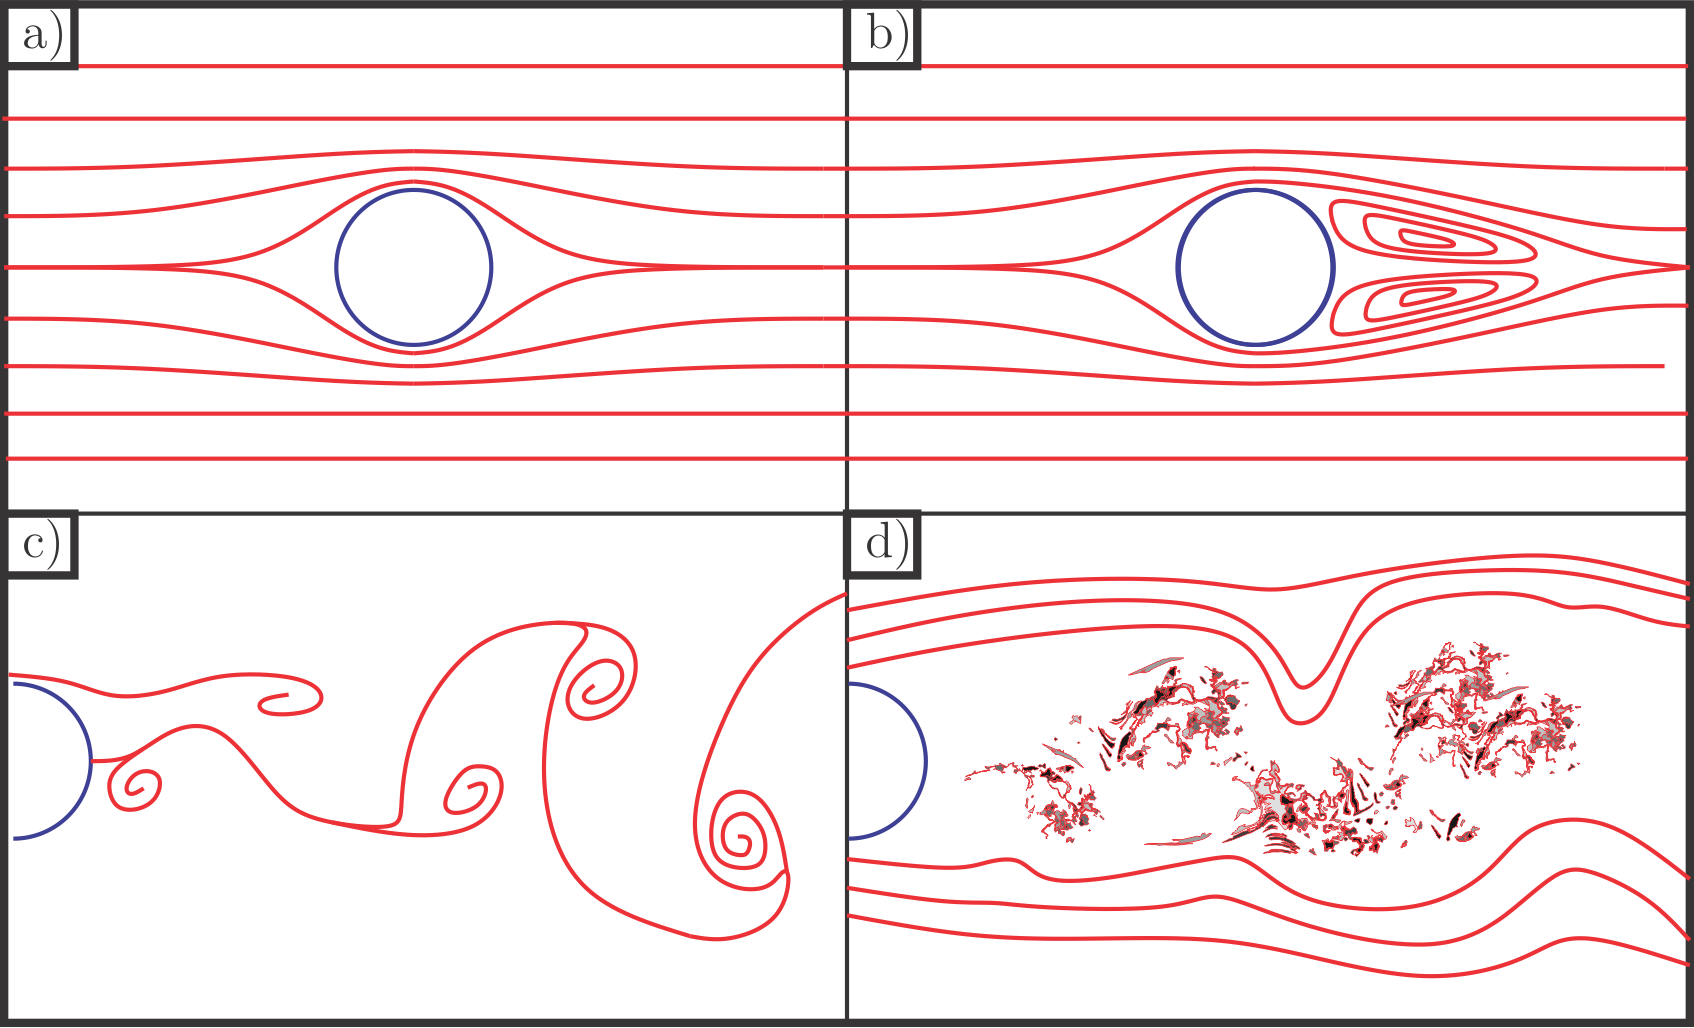
\includegraphics[scale=1]{simetrias}
	\end{center}
	\caption{Esquema de flujo en torno a un cilindro para distintos números de Reynolds. a) $Re\sim 1$, b) $Re \sim 10$, c) $Re\sim 10^2$ y d) $Re\sim 
		10^4$   }
	\label{fig-sim}
\end{figure}

Las ecuaciones de Navier-Stokes poseen un conjunto de simetrías de las cuales podemos observar (esquemáticamente) algunas en la figura \ref{fig-sim}. Las simetrías observadas son,
\begin{itemize}
	\item Invarianza con respecto a traslaciones temporales  
	\item Invarianza bajo reflexiones respecto al eje vertical
	\item Invarianza bajo traslaciones respecto al eje horizontal
	\item Invarianza bajo traslaciones en el eje perpendicular a la figura (eje del cilindro)
\end{itemize}

La invarianza bajo reflexiones con respecto al eje vertical puede ser observada en el caso a), sin embargo ésta no es una simetría de las ecuaciones y por lo tanto solo es aproximada para valores de $Re$ muy bajos. \\
En el caso de reflexiones horizontales, tanto a) como b) presentan ésta simetría, la cual se rompe a medida que aumentamos el número de Reynolds. Cuando llegamos al caso c) también ocurre un cambio en la invarianza bajo traslaciones temporales que en los casos a) y b) es continua, mientras que en c) pasa a ser discreta. \\
Finalmente en el caso d), luego de la transición turbulenta, no existe ninguna simetría. Sin embargo para números de Reynolds altos, se recuperan las simetrías pero en un sentido estadístico, de ahí la importancia de una descripción estadística de la turbulencia. \\
Concretamente, dada una transformación $\hat{g}$ actuando sobre una solución $\vb{v}(t,\vb{r})$, entonces, como índica Frisch \parencite{frisch1995} las ecuaciones de NS poseen las siguientes simetrías conocidas (considerando que las solucionamos en una caja periódica de lado $L$),
\begin{itemize}
	\item Traslaciones espaciales, $\hat{g}_{\rho}:t,\vb{r},\vb{v}\to t,\vb{r}+\vb{\rho},\vb{v}$ 
	\item Traslaciones temporales, $\hat{g}_{\tau}:t,\vb{r},\vb{v}\to t+\tau,\vb{r},\vb{v}$ 
	\item Transformaciones de Galileo, $\hat{g}_{U}:t,\vb{r},\vb{v}\to t+\tau,\vb{r}+\vb{U}t,\vb{v}+\vb{U}$
	\item Paridad, $\hat{g}_{P}:t,\vb{r},\vb{v}\to t,-\vb{r},-\vb{v}$
	\item Rotaciones, $\hat{g}_{R}:t,\vb{r},\vb{v}\to t,\hat{R}\vb{r},\hat{R}\vb{v}$  
	\item Escalamiento $\hat{g}_{S}:t,\vb{r},\vb{v}\to \lambda^{1-h},\lambda\vb{r},\lambda^{h}\vb{v}$  
\end{itemize} 

Es importante mencionar que la simetría bajo rotaciones se mantiene solo si $L\to \infty$ y la de escalamiento en el caso de las ecuaciones de NS solo es válida si $h=-1$ para viscosidad finita. \\
Además es importante recalcar que, como es lógico de esperar, éstas simetrías dependen de las condiciones de borde (el listado anterior es válido para condiciones de borde periódicas). Claramente en el caso de la figura \ref{fig-sim} no habrá invarianza bajo traslaciones espaciales (la velocidad muy cerca de la pared es totalmente distinta a la velocidad en la estela del cilindro), pero si las condiciones de borde tuvieran una simetría discreta, ésta si podría ser heredada por las soluciones (en el caso turbulento de alto Reynolds, hablando en sentido estadístico). Como es de esperar


\pagebreak

\section{Balance de energía}

En el análisis de la turbulencia hay dos tipos de balance que podemos realizar, el primero es un balance global y uno local. El segundo es particularmente útil dado que nos permite analizar como se transfiere la energía entre las distintas escalas. El balance global es simplemente,
\begin{equation*}
	\partial_t E=-\langle \epsilon\rangle+\langle W \rangle
\end{equation*}
Donde $\langle \epsilon\rangle$ representa la energía disipada por la viscosidad, cuya expresión es \parencite{mccomb2014},

\begin{equation*}
	\langle \epsilon\rangle=\frac{\nu}{2}\sum_{ij} \langle \left(\partial_i v_j +\partial_j v_i\right)^2 \rangle 
\end{equation*}
Esta expresión en el caso isótropo se reduce a,
\begin{equation}
	\langle \epsilon\rangle=2\nu\sum_{ij} \langle \left(\partial_i v_j\right)^2 \rangle \label{eq.diss1}
\end{equation} 
Mientras que $W$ es el trabajo realizado por la fuerza externa, dado por,
\begin{equation*}
	W=\langle\vb{f}\cdot \vb{v}\rangle
\end{equation*} 
Nuevamente aprovecharemos el tensor de correlación de un punto (por esto es tan útil definir las correlaciones, contienen información sobre diversas cantidades necesarias en el análisis de la turbulencia) para poder expresar ésta cantidad. Recordemos que,
\begin{equation*}
	R(\vb{r})=\int R_{ij}(\vb{k}) e^{i\vb{k}\cdot\vb{r}}d^3k 
\end{equation*}  
 Entonces vemos que \parencite{pope2001}, 
 \begin{equation*}
 	\langle \partial_m u_i \partial_n u_j\rangle(\vb{r}=\vb{0})=\int k_m k_n R_{ij}(\vb{k}) d^3 k
 \end{equation*}
 Por lo tanto en el caso de la ecuación \ref{eq.diss1} tenemos,
 \begin{equation*}
 	\langle\epsilon\rangle=\int 2\nu k^2R_{ii} dk
 \end{equation*}
 y esto se puede expresar en términos del espectro de energía como,
\begin{equation*}
	\langle\epsilon\rangle=\int 2\nu k^2E(k)dk
\end{equation*}
Un aspecto útil del balance general es que claramente el término no-lineal no introduce energía al sistema, sin embargo como veremos en el balance local si cumple un rol importante redistribuyendo energía entre las escalas.

\subsection{Balance local de energía}

Primero analizaremos el balance de energía utilizando el enfoque de Frisch \parencite{frisch1995}. Para esto introducimos el operador de filtro paso bajo $\hat{P}_{k_0,<}$, el cual posee las siguientes propiedades,
\begin{itemize}
	\item $\hat{P}_{k_0,<}$ conmuta con los operadores diferenciales $\nabla$ y $\nabla^2$
	\item Es autoadjunto $\langle f \hat{P}g \rangle=\langle (\hat{P}f) g \rangle$
\end{itemize}
 Las funciones además se pueden descomponer como $\vb{v}=\vb{v}_{<}+\vb{v}_{>}$, entonces después de aplicar el operador filtro tenemos,
 \begin{equation*}
 	\hat{P}_{k_0,<}\vb{v}=\vb{v}_{k_0,<}
 \end{equation*}
 Donde $k_0$ indica el número de onda en el cual se filtra la función. \\
 Por que és útil utilizar éste operador? Debemos tener en cuenta que la turbulencia es un fenómeno de escalas, existen escalas con estructuras grandes y pequeñas. Las grandes estructuras corresponden a valores pequeños de $k$, dado que $k\sim 1/r$ y viceversa.\\
  Para comprender mejor la aplicación del filtro es útil observar la figura \ref{fig-filtro}. Observamos en la figura superior una señal completa que corresponde a una componente de la velocidad medida en una extensión espacial (notar que el eje horizontal corresponde a una componente espacial). Al aplicar el filtro paso bajo $\hat{P}_{k_0,<}$ solo conservaremos las grandes estructuras (en la figura mostradas en azul) mientras que ignoramos la contribución sobre todas las estructuras tales que $k>k_0$, es decir, las estructuras más pequeñas. 
 
 \begin{figure}[H]
 	\begin{center}
 		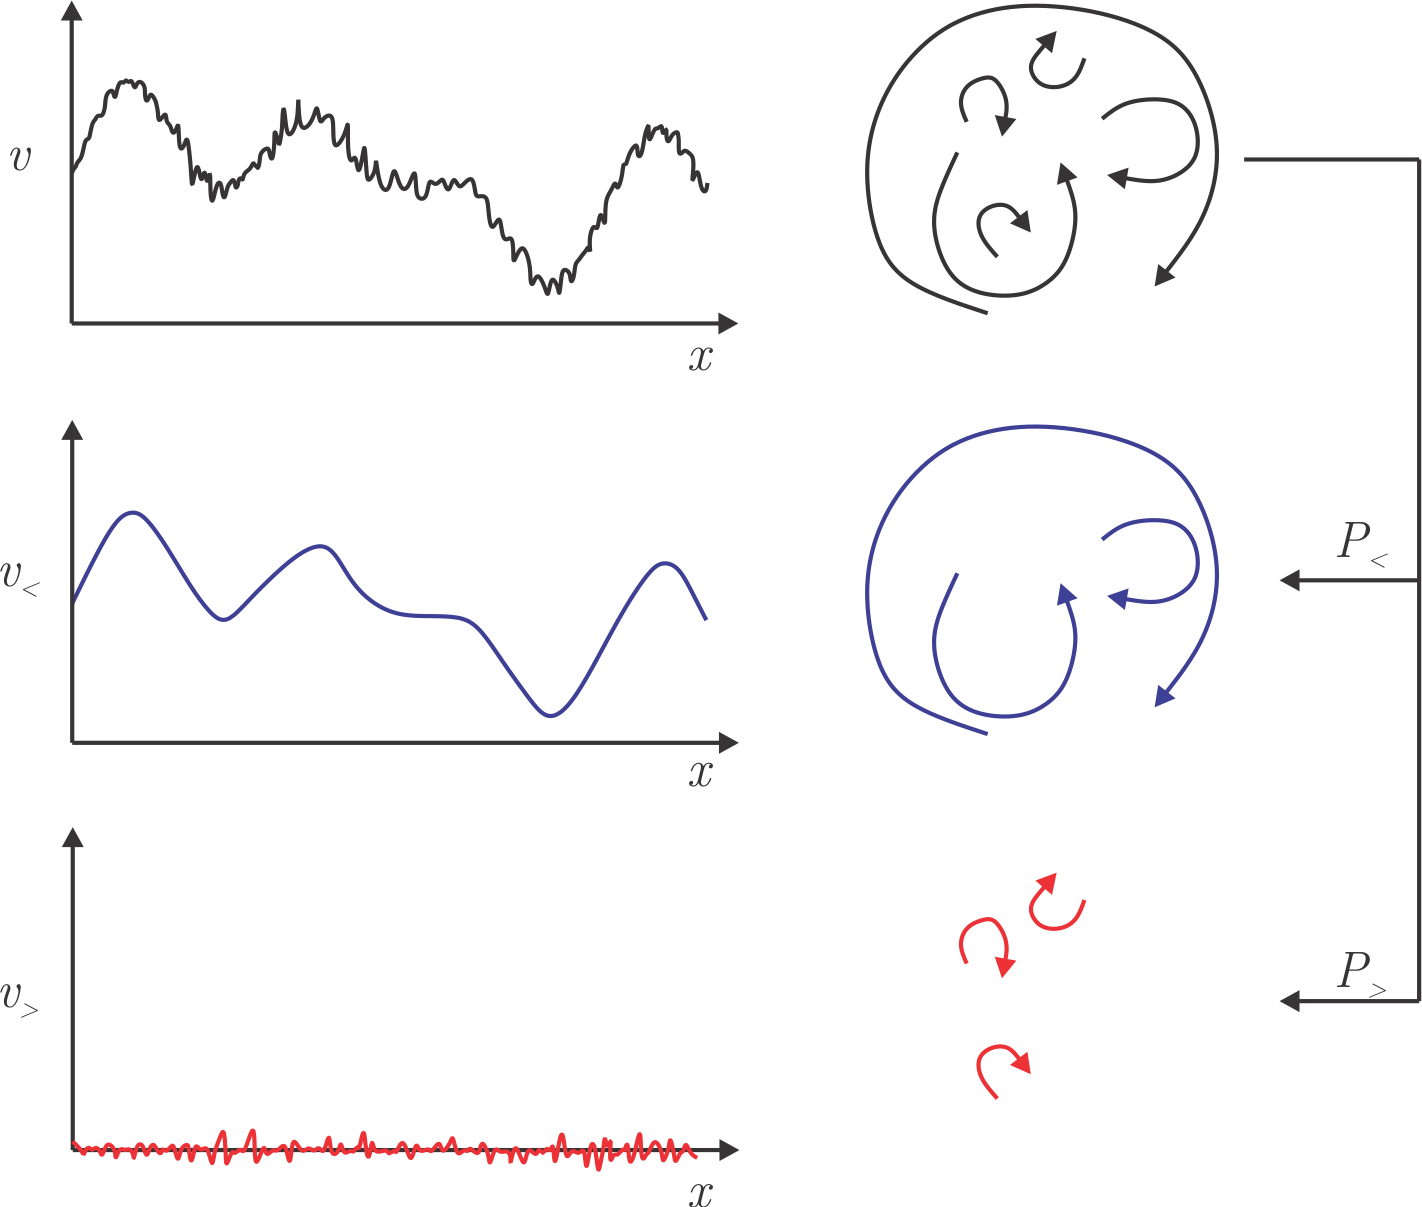
\includegraphics[scale=0.9]{energyBalance}
 	\end{center}
 	\caption{Esquema de la cascada de energía en la teoría K41. }
 	\label{fig-filtro}
 \end{figure}
 
 Ahora consideremos las ecuaciones de NS, 
 \begin{equation*}
 	\partial_t \vb{v}+(\vb{v}\cdot\vb{\nabla})\vb{v}=-\frac{1}{\rho}\vb{\nabla}p+\nu\nabla^2\vb{v}+\vb{f}
 \end{equation*}
 Si aplicamos el filtro paso bajo tendremos,
 \begin{equation*}
 	\partial_t \vb{v}_{k_0,<}+\hat{P}_{k_0,<}\left[(\vb{v}_{k_0,<}+\vb{v}_{k_0,>})\cdot\vb{\nabla}\right](\vb{v}_{k_0,<}+\vb{v}_{k_0,>})=-\frac{1}{\rho}\vb{\nabla}p_{k_0,<}+\nu\nabla^2\vb{v}_{k_0,<}+\vb{f}_{k_0,<}
 \end{equation*}
 Al tomar el producto escalar con $\vb{v}_{k_0,<}$ y promediar tenemos,
 \begin{align*}
 	&\langle \vb{v}_{k_0,<} \cdot \partial_t \vb{v}_{k_0,<} \rangle+\langle \vb{v}_{k_0,<} \cdot \hat{P}_{k_0,<}\left[(\vb{v}_{k_0,<}+\vb{v}_{k_0,>})\cdot\vb{\nabla}\right](\vb{v}_{k_0,<}+\vb{v}_{k_0,>})\rangle\\
 	&=-\frac{1}{\rho}\langle\vb{v}_{k_0,<}\cdot\vb{\nabla}p_{k_0,<}\rangle+\nu\langle \vb{v}_{k_0,<}\cdot\nabla^2\vb{v}_{k_0,<}\rangle+\langle \vb{v}_{k_0,<}\cdot \vb{f}_{k_0,<}\rangle
 \end{align*}
 
 Para el primer término tenemos,
 \begin{equation*}
 	\vb{v}_{k_0,<} \cdot \partial_t \vb{v}_{k_0,<}=\partial_t\left(\frac{1}{2}\vb{v}_{k_0,<}^2\right)
 \end{equation*}
 Para el segundo término podemos aplicar la propiedad autoadjunta del operador y además es claro que $\hat{P}_{k_0,<}\vb{v}_{k_0,<}=\vb{v}_{k_0,<}$, por lo tanto,
 \begin{align*}
 	&\langle \vb{v}_{k_0,<} \cdot \hat{P}_{k_0,<}\left[(\vb{v}_{k_0,<}+\vb{v}_{k_0,>})\cdot\vb{\nabla}\right](\vb{v}_{k_0,<}+\vb{v}_{k_0,>})\rangle\\
 	&=\langle \hat{P}_{k_0,<}\vb{v}_{k_0,<} \cdot \left[(\vb{v}_{k_0,<}+\vb{v}_{k_0,>})\cdot\vb{\nabla}\right](\vb{v}_{k_0,<}+\vb{v}_{k_0,>})\rangle\\
 	&=\langle \vb{v}_{k_0,<} \cdot \left[(\vb{v}_{k_0,<}+\vb{v}_{k_0,>})\cdot\vb{\nabla}\right](\vb{v}_{k_0,<}+\vb{v}_{k_0,>})\rangle
 \end{align*}
 
 y este producto se puede expandir como,
 \begin{align*}
 	&\langle \vb{v}_{k_0,<} \cdot \left[(\vb{v}_{k_0,<}+\vb{v}_{k_0,>})\cdot\vb{\nabla}\right](\vb{v}_{k_0,<}+\vb{v}_{k_0,>})\rangle\\
 	&=\langle \vb{v}_{k_0,<} \cdot \left[\vb{v}_{k_0,<}\cdot\vb{\nabla}\right]\vb{v}_{k_0,<}\rangle+\langle \vb{v}_{k_0,<} \cdot \left[\vb{v}_{k_0,<}\cdot\vb{\nabla}\right]\vb{v}_{k_0,>}\rangle\\
 	&+\langle \vb{v}_{k_0,<} \cdot \left[\vb{v}_{k_0,>}\cdot\vb{\nabla}\right]\vb{v}_{k_0,<}\rangle+\langle \vb{v}_{k_0,<} \cdot \left[\vb{v}_{k_0,>}\cdot\vb{\nabla}\right]\vb{v}_{k_0,>}\rangle
 \end{align*}
 Ahora, para simplificar la notación denotamos las componentes de $\vb{v}_{k_0,<}$ como $f_i$ y las de $\vb{v}_{k_0,>}$ como $g_i$, entonces tendremos para el primer término,
 \begin{align*}
    \langle f_i f_j \partial_j f_i \rangle &= \langle \partial(f_if_jf_i) \rangle-\langle f_i \partial_j (f_i f_j) \rangle\\
    &=-\langle f_i f_j \partial_j f_i \rangle-\langle f_i f_i \partial_j f_j \rangle\\
    &=-\langle f_i f_j \partial_j f_i \rangle
 \end{align*} 
 Por lo tanto llegamos a $2\langle f_i f_j \partial_j f_i \rangle=0\implies \langle f_i f_j \partial_j f_i \rangle=0$. En la segunda línea se utiliza la propiedad del promedio que para funciones periódicas $\langle\partial_i f\rangle=0$ (\parencite{frisch1995}) y en la tercera línea se utiliza la condición de incompresibilidad. Lo mismo se puede realizar para el tercer término y llegamos a,
 \begin{equation*}
 	\langle \vb{v}_{k_0,<} \cdot \left[(\vb{v}_{k_0,<}+\vb{v}_{k_0,>})\cdot\vb{\nabla}\right](\vb{v}_{k_0,<}+\vb{v}_{k_0,>})\rangle=\langle \vb{v}_{k_0,<} \cdot \left[\vb{v}_{k_0,<}\cdot\vb{\nabla}\right]\vb{v}_{k_0,>}\rangle+\langle \vb{v}_{k_0,<} \cdot \left[\vb{v}_{k_0,>}\cdot\vb{\nabla}\right]\vb{v}_{k_0,>}\rangle
 \end{equation*}
Otras propiedades útiles son,
\begin{equation*}
	\langle (\partial_i f) g \rangle=-\langle f\partial_i g \rangle \hspace{0.5cm} \langle \vb{u}\cdot \nabla^2\vb{v} \rangle=-\langle (\nabla\times\vb{u})\cdot(\nabla\times\vb{v}) \rangle
\end{equation*}
 Donde la segunda identidad es solo válida en el caso incompresible. De éstas tenemos que, para el término de la presión (donde nuevamente $f_i$ representa las componentes de la velocidad filtrada),
 \begin{equation*}
 	\langle f_i \partial_i p_{k_0,<}\rangle=-\langle  p_{k_0,<}  \partial_i f_i\rangle=0
 \end{equation*}
 Donde en la última igualdad se utiliza la condición de incompresibilidad. Para el término que acompaña la viscosidad se tiene,
 \begin{equation*}
 	\nu\langle \vb{v}_{k_0,<}\cdot\nabla^2\vb{v}_{k_0,<}\rangle=-\nu\langle\vb{\omega}_{k_0,<}^2\rangle
 \end{equation*}
 Donde se utilizó una de las propiedades mencionadas anteriormente. Luego de esto, podemos escribir una ecuación de balance como,
 \begin{equation*}
 	\partial_t E_{k_0}+\Pi_{k_0}=-2\nu\Omega_{k_0}+W_{k_0} 
 \end{equation*}
 Donde todas las cantidades son acumuladas desde $k=0$ hasta $k_0$, observamos que tenemos términos que corresponden a la disipación y al trabajo realizado por la fuerza externa, tal como en el balance global, pero ahora además tenemos el término  $\Pi_{k_0}$,
 \begin{equation*}
 	\Pi_{k_0}=\langle \vb{v}_{k_0,<} \cdot \left[\vb{v}_{k_0,<}\cdot\vb{\nabla}\right]\vb{v}_{k_0,>}\rangle+\langle \vb{v}_{k_0,<} \cdot \left[\vb{v}_{k_0,>}\cdot\vb{\nabla}\right]\vb{v}_{k_0,>}\rangle
 \end{equation*}
 
 Observamos que éste término proviene de la parte no-lineal, su rol por lo tanto es transportar la energía entre las distintas escalas. La ventaja de ésta formulación es que no se asumió homogeneidad o isotropía, por lo que es general. 
\section{Teoría de Kolmogorov y cascada de energía}



La primera noción sobre una cascada de energía (en aspectos formales) fue dada por Richardson. Una de las principales búsquedas en la turbulencia es de universalidad en alguna característica estadística del problema. El primer aporte de Richardson fue sugerir que, si existe universalidad, debe ser en la diferencia de velocidades entre 2 puntos \parencite{lvov1995}, de aquí la importancia de las funciones de estructura. Esto debido a que al tomar la diferencia de las velocidades en 2 puntos, se eliminan las contribuciones de las estructuras mayores a la distancia entre ambos, y, por lo tanto, la dependencia en la escala a la cual es inyectada la energía (ésta que, obviamente no es universal dado que depende del problema). Esto por lo tanto, elimina la opción de que el campo de velocidades (o cualquier estadística de un punto) pueda ser universal. \\

\subsection{Ley de 2/3}
La teoría de Kolmogorov de 1941 (conocida como K41) se basa en 3 supuestos \parencite{kolmogorov1941a},
\begin{itemize}
	\item En escalas suficientemente pequeñas ($r \ll L$, donde $L$ es la escala del forzamiento)la turbulencia presenta isotropía y homogeneidad local.
	\item En escalas pequeñas $r\ll L$ las características dinámicas que describen el flujo solo pueden depender de la disipación de energía, $\langle \epsilon\rangle$ y la viscosidad $\nu$.
	\item Existe una escala intermedia $\ell$ (llamada rango inercial) la cual está lo suficientemente lejos de la pequeña escala de disipación $\eta$ y la de forzamiento $L$ ($\eta \ll \ell\ll L $). En este rango las características del flujo solo dependen de la disipación $\langle \epsilon\rangle$ , además ésta presenta una invarianza de escala.
\end{itemize}


\begin{figure}[H]
	\begin{center}
		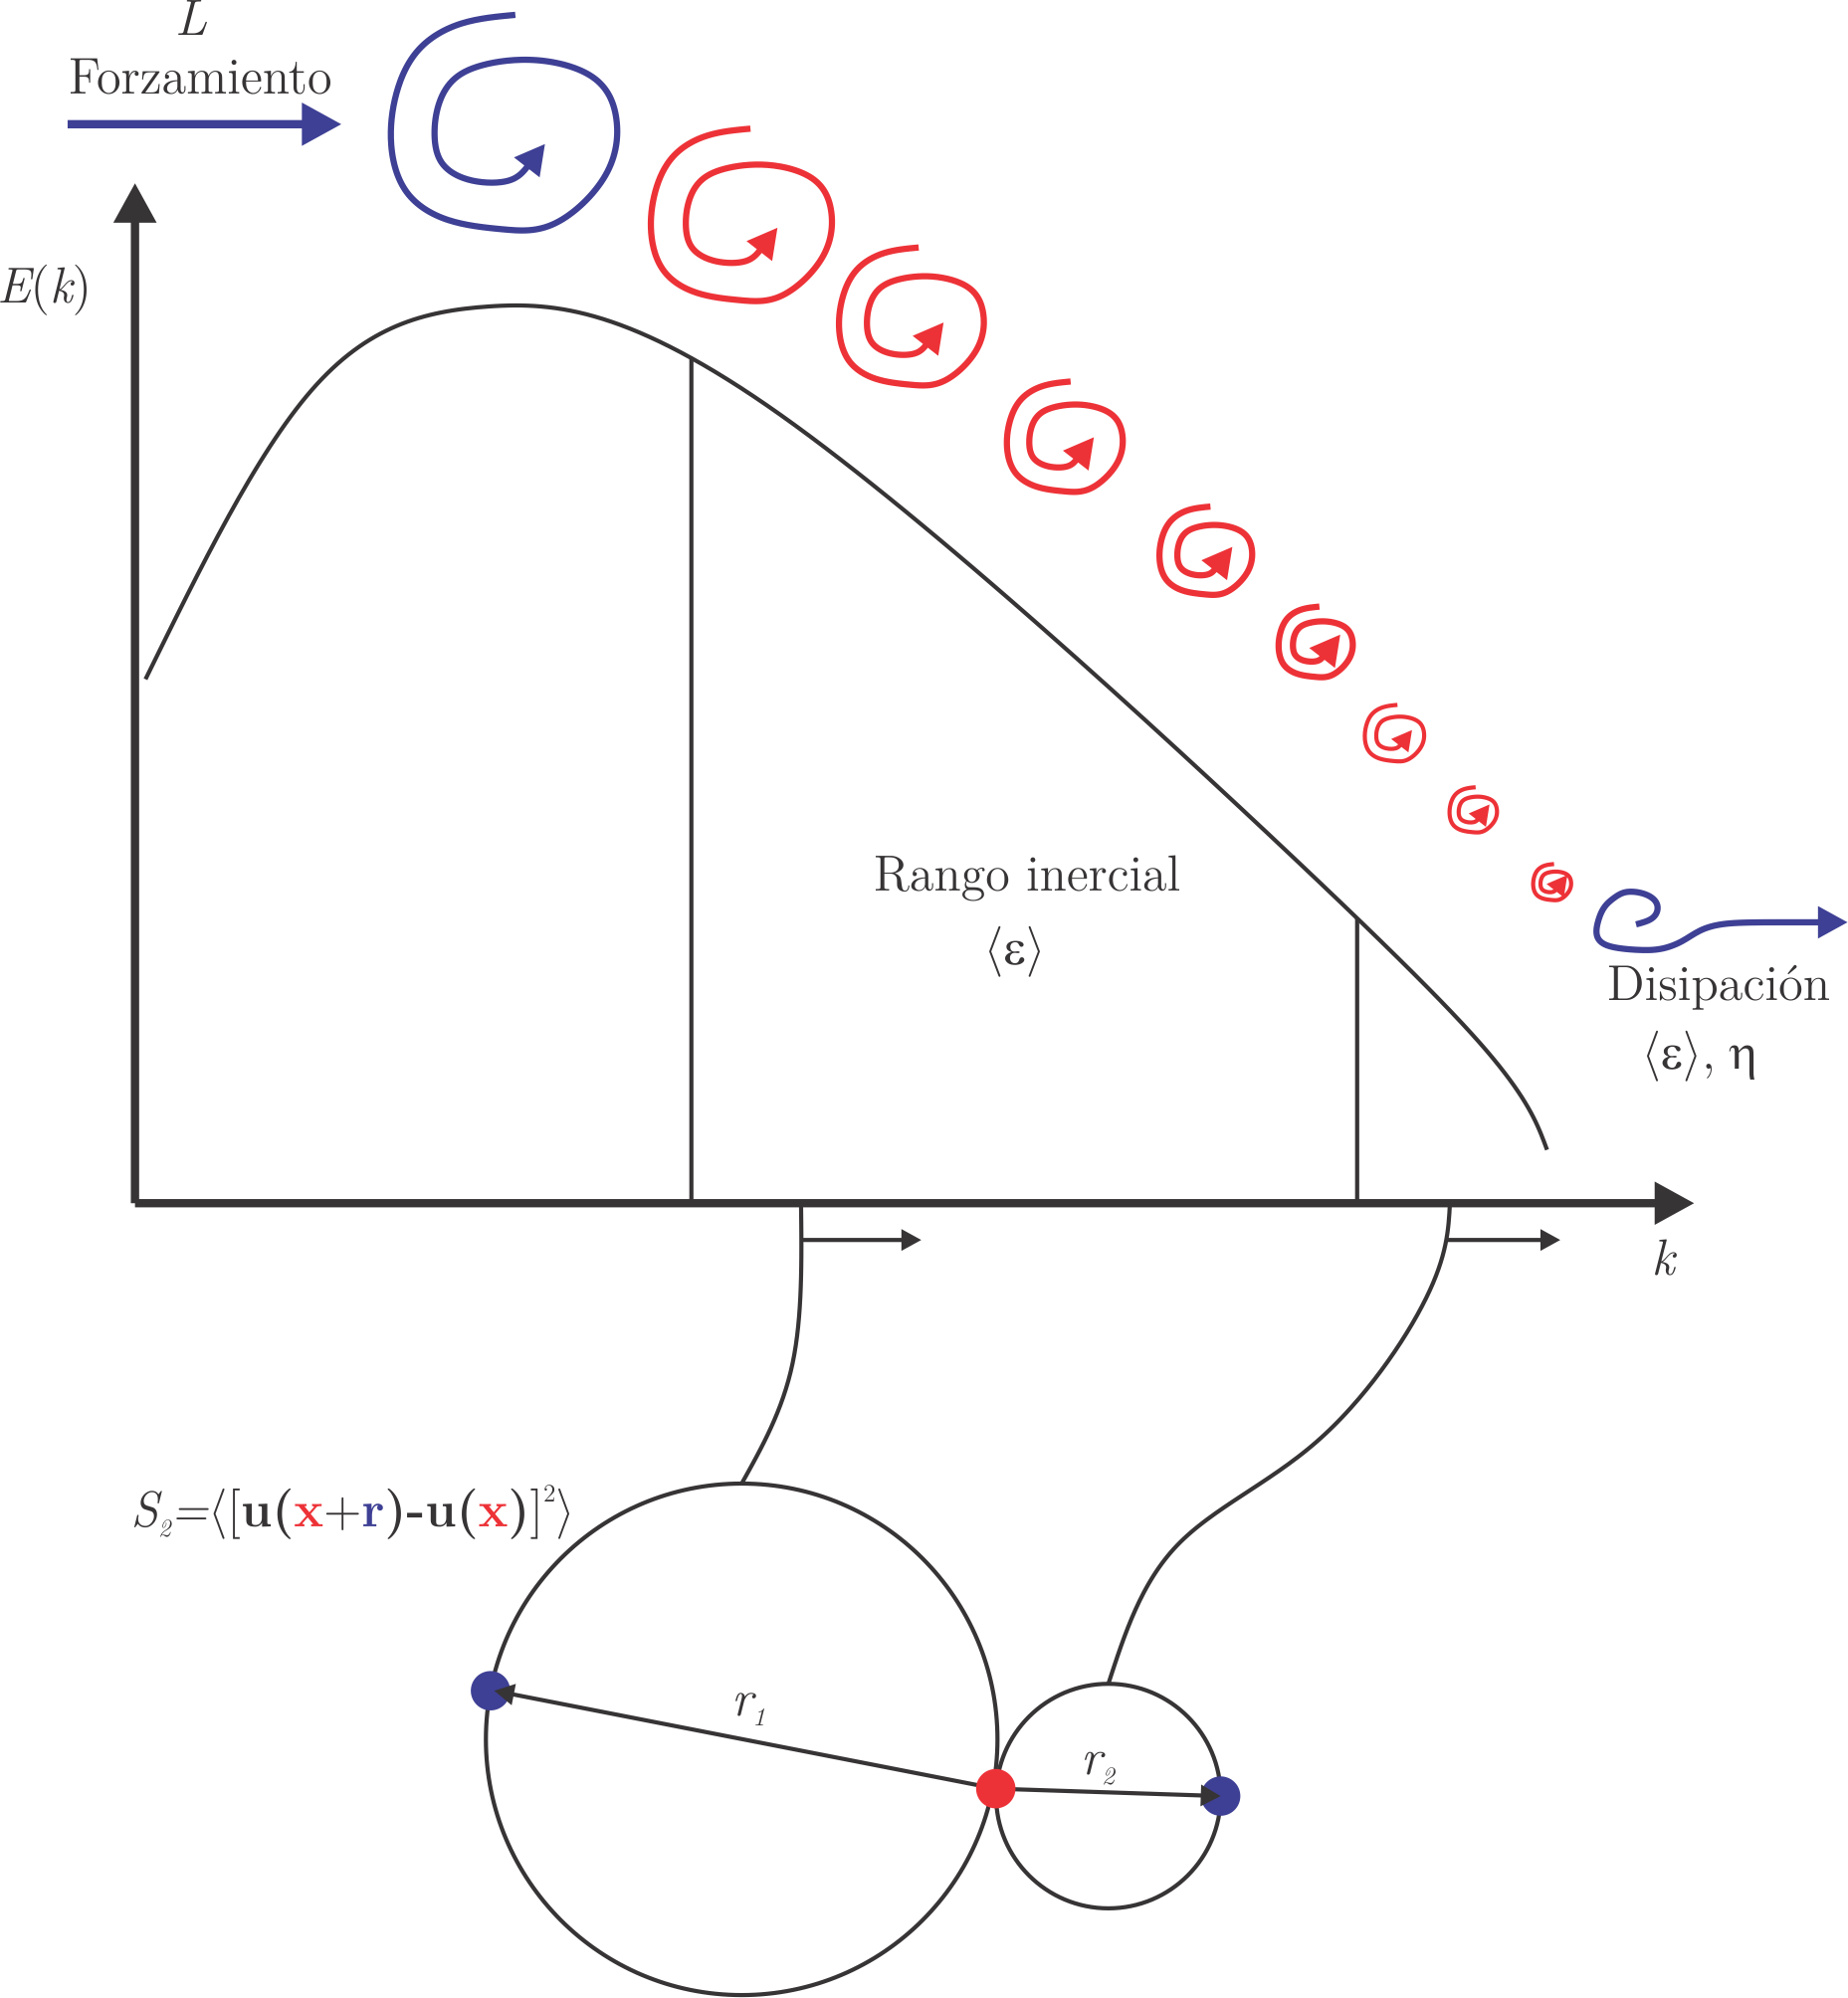
\includegraphics[scale=0.9]{k41}
	\end{center}
	\caption{Esquema de la cascada de energía en la teoría K41. }
	\label{fig-k41}
\end{figure}

En la figura \ref{fig-k41} se muestra de forma esquemática el espectro de energía $E(k)$ y la cascada que se produce desde las escalas grandes $L$ hacia las escalas pequeñas $\eta$. También se muestra un esquema de las funciones de estructura, según lo propuesto por Richardson, éstas solo contendrán información sobre escalas menores al circulo del radio $\vb{r}$. \\
A partir de la teoría de Kolmogorov entonces podemos decir que en las escalas pequeñas solo existirá una dependencia de $\nu$ y $\langle \epsilon \rangle$. Ahora, las unidades de éstas cantidades son, 
\begin{equation*}
	\left[ \epsilon \right] = L^2 T^{-3} \hspace{0.5cm} \left[\nu\right]=L^2T^{-1}
\end{equation*} 
Donde $L$ representa unidades de longitud y $T$ unidades de tiempo. Por lo tanto, si queremos formar una escala de longitud de disipación, mediante análisis dimensional podemos ver que se debe cumplir,

\begin{equation*}
	\left[\langle \epsilon \rangle^m \nu^n \right]= L^{2n}T^{-n}L^{2m}T^{-3m}=L^1 T^0  
\end{equation*}

De esto obtenemos las ecuaciones,
\begin{equation*}
	2n-2m=1 \hspace{0.5cm} n+3m=0
\end{equation*}

Cuyas soluciones son $n=3/4$ y $m=-1/4$, por lo que formamos nuestra escala de disipación (también conocida como escala de Kolmogorov),
 

\begin{equation*}
\eta=\frac{\nu^{3/4}}{\langle \epsilon \rangle ^{1/4}}=\left(\frac{\nu^3}{\langle \epsilon \rangle}\right)^{1/4} 
\end{equation*}

De la misma forma, para la función de estructura de segundo orden tenemos, 

\begin{equation*}
	\left[S_2\right]=L^2 T^{-2}
\end{equation*}

Entonces, en el rango inercial sabemos que ésta solo dependerá de $\vb{r}$ y $\langle \epsilon \rangle$ (por la hipótesis de existencia del rango inercial), por lo tanto del análisis dimensional tendremos,
\begin{equation*}
	L^{2m} T^{-3m}L^{n}=L^2T^{-2}
\end{equation*} 
De lo cual obtenemos las ecuaciones,
\begin{equation*} 
	2m+n=2\hspace{0.5cm} -3m=-2
\end{equation*}
Cuyas soluciones son, $m=2/3$ y $n=2/3$, por lo que en el rango inercial la función de estructura tendrá la forma,
\begin{equation*}
	S_2=C\langle \epsilon \rangle^{2/3}r^{2/3}
\end{equation*}
En general, las funciones de estructura de orden $n$ tienen la forma (de acuerdo a la teoría de Kolmogorov),

\begin{equation*}
	S_n(\vb{r})=C_n\left(\langle\epsilon\rangle\right)^{n/3}
\end{equation*}


Ahora, también podemos analizar la teoría de Kolmogorov desde el punto de vista de las simetrías proponiendo las siguientes hipótesis,

\begin{itemize}
	\item Lejos de las fronteras, en el límite $Re\to \infty$, las simetrías rotas por los mecanismos que producen la turbulencia son restauradas en escalas suficientemente pequeñas.
	\item Lejos de las fronteras, en el límite $\Re\to\infty$ el fluido presenta un comportamiento autisimilar en las pequeñas escalas. Esto es, existe $h \in \real$ tal que,
	\begin{equation*}
		\vb{v}(\vb{x}+\lambda \vb{r})-\vb{v}(\vb{x})=\lambda^h \left[\vb{v}(\vb{x}+\vb{r})-\vb{v}(\vb{x})\right]
	\end{equation*}
	
	\item En el límite $Re \to \infty$, existe una disipación de energía no nula. 
\end{itemize}

El punto sobre la existencia de una disipación de energía no-nula en el límite $\nu\to 0$ ($Re\to \infty$) es uno muy importante, este fenómeno es conocido como anomalía disipativa o disipación anómala. Lo interesante es que, en el límite $\nu\to 0$ uno esperaría (a pretorio) que las ecuaciones de NS converjan a las ecuaciones de Euler para fluidos inviscidos, sin embargo se observa que sin importar lo pequeña que sea la viscosidad, siempre existe disipación de energía. \\
Desde este punto de vista, la teoría de Kolmogorov y los exponentes $n/3$ en realidad son parte de algo más profundo que un simple análisis dimensional. Onsager \parencite{onsager1949,eyink2006} menciona que la diferencia de velocidades no debe satisfacer ninguna condición de la forma 
\begin{equation*}
	\abs{\vb{v}(\vb{x}+\vb{r})-\vb{v}(\vb{x})}\le C r^\zeta
\end{equation*}
para $\zeta>1/3$, dado que si eso ocurre, la energía será una cantidad conservada (y por lo tanto $\langle \epsilon\rangle\to 0$ cuando $\nu\to 0$). En general para la función de estructura de orden $n$, el máximo valor que puede tomar el exponente es $n/3$, por lo que la teoría de Kolmogorov toma el máximo valor para el cual existe una disipación anómala (la cual está demostrada experimentalmente).\\

La teoría de Kolmogorov además nos entrega información importante sobre la fenomenología de la turbulencia, particularmente sobre la existencia de una cascada directa de energía (tal como había propuesto Richardson).\\
 Para que pueda existir un fenómeno de tipo cascada (estos también ocurren en otras cantidades conservadas, como la enstrofía o la helicidad y no siempre son directas \parencite{alexakis2018}) debe haber un flujo local de la cantidad, es decir, solo se debe transmitir entre escalas cercanas. \\
 El argumento usual (fenomenológico) para argumentar la localidad de las interacciones se basa en separar la interacción de las estructuras de orden $\sim \ell$ (en el rango inercial) en dos tipos, el primero es un arrastre debido a las estructuras grandes (en ingles \textit{sweeping}) y el segundo es una interacción que si produce distorsión de las estructuras debido al esfuerzo de corte.     \\
 La primera interacción (de arrastre) debido a escalas $L\gg\ell$ no debería cambiar la estructura ni el contenido de energía de estructuras del orden $\sim \ell$, además si el arrastre es uniforme, no produce variaciones en las estructuras finas debido a la invarianza bajo transformaciones de Galileo de las ecuaciones de NS (el efecto es similar a ver la estructura pequeña desde un marco de referencia moviéndose a velocidad constante). \\
 La segunda interacción descrita es debido al esfuerzo de corte (gradientes de velocidad), éste es del orden \parencite{frisch1995},
 \begin{equation*}
 	s_{\ell}\sim \frac{v_{\ell}}{\ell}\sim \langle\epsilon\rangle^{1/3}\ell^{-2/3}
 \end{equation*}
Se argumenta que las estructuras de escalas $L\gg \ell$ no generan una distorsión considerable debido a que el esfuerzo de corte es pequeño en escalas grandes, mientras que las escalas pequeñas ($\eta\ll \ell$) no afectan porque la correlación entre ambas escalas es baja. Estos argumentos entonces sirven para decir que la mayor parte de las contribuciones al flujo de energía en una escala $\ell$ vienen de las escalas cercanas y por lo tanto existe una cascada de energía porque existe localidad en las interacciones.\\

Un punto importante es que la cascada de energía es un fenómeno en el espacio de Fourier, pero no se debe tener la imagen en el espacio real de una estructura grande rompiéndose en otras más pequeñas, como explican Sagaut y Tsinober \parencite{sagaut2008,tsinober2009} en el espacio físico se debe reemplazar la imagen de cascada por una de generación de gradientes de velocidad. Una mejor imagen de como realmente ocurren los procesos y la generación de pequeñas escalas en la turbulencia puede ser obtenida observando experimentos modernos (numéricos o experimentales), éstos generalmente están enfocados en la colisión de tubos de vórtices para analizar como a partir de ésto nacen estructuras pequeñas \parencite{rubinstein2018,yao2020}. 
  


\subsection{Escalamiento anómalo}

A pesar del éxito de la teoría de Kolmogorov, se sabe que ésta no es correcta. Los exponentes de las funciones de estructura no aumentan como $n/3$ para $n>3$ \parencite{lvov1996}. Tal como fue explicado en el capitulo anterior, los exponentes que predice la teoría de Kolmogorov corresponden a un caso muy particular, dado que son el máximo valor para el cual la disipación de energía se mantiene finita en el límite $\nu\to0$. \\
Se ha observado experimentalmente \parencite{lvov1996} que para debe haber una dependencia de las funciones de estructura en las grandes escalas $L$ para tener en cuenta los exponentes anómalos,
\begin{equation*}
	S_n(r)\sim C_n \langle\epsilon\rangle^{n/3}r^{n/3}\left(\frac{r}{L}\right)^{\zeta_a}
\end{equation*} 

Donde $\zeta_a$ representa el exponente anómalo. Como explica \parencite{eyinkLecture}, esto significa que la información sobre las grandes escalas no es perdida en el proceso de cascada. Ésto se debe al fenómeno de la intermitencia, que corresponde a \textit{peaks} (negativos o positivos) en diferentes cantidades, esto es, eventos extremos. Esto genera la no-Gaussianidad de las funciones distribuciones de probabilidad, dado que en las pequeñas escalas existe una probabilidad mayor (respecto a una distribución Gaussiana) de ocurrencia de eventos extremos.  

\begin{figure}[H]
	\begin{center}
		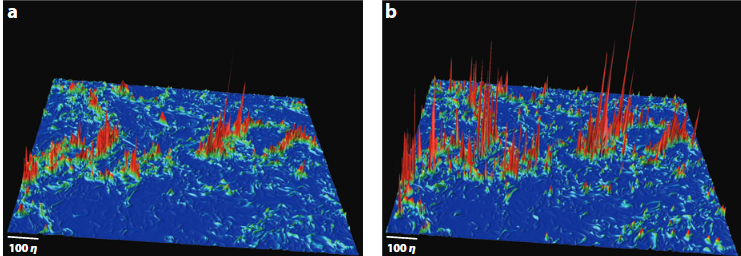
\includegraphics[scale=0.75]{interm1}
	\end{center}
	\caption{Distribución de disipación de energía (izquierda) y enstrofía (derecha) obtenidas por Ishihara et al. \parencite{ishihara2009}. En ambos casos se puede observar la intermitencia como \textit{peaks} de pequeña escala. }
	\label{fig-interm1}
\end{figure}



\subsection{Ecuación de Karman-Howarth}

Hasta ahora hemos descrito parte de la teoría estadística de la turbulencia. Como hemos visto los puntos centrales de ésta son las funciones de correlación (o de estructura), por lo que parece lógico obtener una ecuación que describa la evolución de éstas.\\
Con el fin de obtener ésta ecuación consideremos la velocidad en dos puntos $\vb{x}$ y $\vb{x}'=\vb{x}+\vb{r}$, entonces denotamos las componentes de la velocidad en estos puntos por $v_i$ y $v_i'$ respectivamente (y las derivadas por $\partial_i$ y $\partial_i'$). Entonces multiplicando la ecuación de Navier-Stokes por $v_j'$, 
\begin{equation*}
	v_j'\partial_tv_i+v_j'v_k\partial_kv_i=-\frac{1}{\rho}v_j'\partial_i p + \nu v_j'\partial_k\partial_k v_i 
\end{equation*}
Ahora consideremos el promedio de ésta ecuación y la sumamos con la ecuación para las variables en $\vb{x}'$ multiplicadas por $v_i$, 

\begin{equation*}
\langle v_j'\partial_tv_i \rangle+\langle v_i\partial_tv_j' \rangle+\langle v_j'v_k\partial_kv_i\rangle+\langle v_iv_k'\partial_k'v_j'\rangle=-\frac{1}{\rho}\langle v_j'\partial_i p \rangle-\frac{1}{\rho}\langle v_i\partial_j' p \rangle + \nu \langle v_j'\partial_k\partial_k v_i \rangle+\nu \langle v_i\partial_k'\partial_k' v_j' \rangle
\end{equation*}

Ahora, esto se puede reescribir como,
\begin{equation*}
	\partial_t\langle v_iv_j' \rangle+\underbrace{\langle v_k\partial_kv_iv_j'\rangle+\langle v_k'\partial_k'v_j'v_i\rangle}_{I}=-\frac{1}{\rho}(\langle v_j'\partial_i p \rangle+\langle v_i\partial_j' p \rangle )+ \nu (\langle\partial_k\partial_k v_i v_j' \rangle+\langle \partial_k'\partial_k' v_j'v_i \rangle)
\end{equation*}

Ahora, consideremos el término $I$, 

\begin{align*}
	\langle v_k\partial_kv_iv_j'\rangle&=\partial_k\langle v_kv_iv_j'\rangle-\langle v_iv_j'\partial_kv_k\rangle\\
	&=\partial_k\langle v_kv_iv_j'\rangle
\end{align*}
Donde se utiliza la condición de incompresibilidad. Lo mismo ocurre para el otro término denotado por $I$ y reescribimos la ecuación como,
\begin{equation*}
	\partial_t\langle v_iv_j' \rangle+\partial_k\langle v_kv_iv_j'\rangle+\partial_k'\langle v_k'v_j'v_i\rangle=-\frac{1}{\rho}(\langle v_j'\partial_i p \rangle+\langle v_i\partial_j' p \rangle )+ \nu (\partial_k\partial_k\langle v_i v_j' \rangle+ \partial_k'\partial_k'\langle v_j'v_i \rangle)
\end{equation*}

El siguiente paso es aplicar las condiciones de isotropía y homogeneidad. Por la isotropía las correlaciones de la presión se anulan \parencite{monin1976,argyris2015}. Ahora, observamos que solo nos quedan correlaciones de 2 puntos, y para el caso homogeneo sabemos que éstas solo dependen de la distancia entre los puntos. Por lo tanto podemos hacer el reemplazo $(\partial_i,\partial_i')\to(-\partial_{r_i},\partial_{r_i})$. Entonces tenemos,


\begin{equation*}
	\partial_t\langle v_iv_j' \rangle+\partial_{r_i}\langle v_k'v_j'v_i\rangle-\partial_{r_i}\langle v_kv_iv_j'\rangle= 2\nu \partial_{r_i}\partial_{r_i}\langle v_j'v_i \rangle
\end{equation*}

O utilizando la notación de los tensores de correlación,
\begin{equation}
	\partial_tR_{ij}+\partial_{r_i}R_{i,jk}-\partial_{r_i}R_{ik,j}= 2\nu \partial_{r_i}\partial_{r_i}R_{ij}
\end{equation}

Ahora recordemos que para el caso isótropo las funciones de estructura radiales (y las de correlación) se pueden expresar solo en términos de una función escalar de $r$. Reemplazando las expresiones y luego de varias manipulaciones a la ecuación resultante, se llega a la siguiente expresión para las funciones de estructura longitudinales,

\begin{equation}
	\pdv{R_{LL}(r,t)}{t}=\left(\pdv{}{r}+\frac{4}{r}\right)\left(R_{LL,L}(r,t)+2\nu\pdv{R_{LL}(r,t)}{r}\right)
	\label{eq.KH.IH}
\end{equation}
 Donde las funciones longitudinales están dadas por,
 
 \begin{equation*}
 	R_{LL}=\langle u_r(\vb{x})u_r(\vb{x}+\vb{r}) \rangle \hspace{0.5cm} R_{LL,L}=\langle u_r(\vb{x})^2u_r(\vb{x}+\vb{r}) \rangle
 \end{equation*}
 En estas funbciones, $u_r$ se refiere a la proyección longitudinal de la velocidad. \\
 Esta es la ecuación de Karman-Howarth para turbulencia isótropa y homogenea. Un punto importante de las ecuaciones anteriores es el acoplamiento entre la correlación de segundo orden con la de tercer orden. 
 
\subsection{Ley de 4/5 de Kolmogorov}

La ley de $4/5$ de Kolmogorov es uno de los pocos resultados analíticos exactos que se pueden obtener a partir de las ecuaciones de Navier-Stokes. Para poder obtenerla debemos expresar la ecuación de Karman-Howarth en términos de las funciones de estructura,

\begin{align*}
	S_2(r)&=\langle \left[u_r(r)-u_r(0)\right]^2 \rangle\\
	&=\langle u_r^2(r) \rangle -2\langle u_r(0)u_r(r) \rangle +\langle u_r^2(0) \rangle\\
	&=2\langle u_r^2(0) -2\langle u_r(0)u_r(r)\\
	&=2(R_{LL}(0)-R_{LL}(r))
\end{align*}

Donde se usa la homegeneidad del campo. Para la función de estructura de tercer orden,

\begin{align*}
	S_r(r)&=\langle \left[u_r(r)-u_r(0)\right]^2 \rangle\\
	&=\langle u_r^3(r) -3u_r^2(r)u_r(0) +3 u_r^2(0)u_r(r)-u_r^3(0) \rangle\\
	&= 3\langle u_r^2(0)u_r(r) - u_r^2(r)u_r(0)   \rangle\\
	&=6R_{LL,L}
\end{align*} 

Ahora, asumiendo las hipótesis de Kolmogorov, cuando $Re\to\infty$ existe una separación de escalas. Si estudiamos solo la pequeña escala, entonces consideramos $r\ll L$. En este escenario podemos considerar que la función de estructura solo depende de la disipación y la viscosidad, por lo tanto su derivada parcial con respecto al tiempo es cero. Debido a esto tenemos entonces,

\begin{equation*}
	\pdv{S_3}{t}=2\pdv{R_{LL}(0,t)}{t} - 2\pdv{R_{LL}(r,t)}{t}=0
\end{equation*}
Para el primer término, sabemos que la correlación está relacionada con la energía cinética por $R_{LL(0,t)}=\frac{2}{3} \pdv{}{t} \langle \frac{u^2}{2}\rangle =-\frac{2}{3}\epsilon$.  Para la derivada temporal de $R_{LL}(r,t)$ simplemente aplicamos la ecuación de Karman-Howarth y llegamos a,

\begin{equation*}
	-\frac{2}{3}\epsilon=\left(\pdv{}{r}+\frac{4}{r}\right)\left(R_{LL,L}(r,t)+2\nu\pdv{R_{LL}(r,t)}{r}\right)
\end{equation*}

Reemplazando $R_{LL,L}=\frac{1}{6}S_3(r)$ y $\pdv{S_2}{r}=-2\pdv{R_{LL}}{r}$, 

\begin{equation*}
	-\frac{2}{3}\epsilon=\left(\pdv{}{r}+\frac{4}{r}\right)\left(\frac{1}{6}S_3(r)-\nu\pdv{S_2(r,t)}{r}\right)
\end{equation*}
Esta ecuación se puede reescribir como,
\begin{equation*}
	\frac{1}{3}\pdv{(r^4 S_3)}{r}=2\nu\pdv{}{r}\left(r^4 \pdv{S_2}{r}\right)-\frac{4}{3}r^4\epsilon
\end{equation*}
Integrando sobre $r$ llegamos a,

\begin{equation*}
	\frac{1}{3}r^4 S_3 =2\nu r^4 \pdv{S_2}{r}-\frac{4}{15}r^5\epsilon
\end{equation*}
Y tenemos la siguiente expresión para la función de estructura de tercer orden, 

\begin{equation*}
	S_3=6\nu S_2-\frac{4}{5}\epsilon r
\end{equation*}
Además dadas las hipótesis de Kolmogorov, en el rango inercial la función solo debería depender de $\epsilon$ por lo tanto para este se tiene la famosa ley de $4/5$ de Kolmogorov,
\begin{equation*}
	S_3=-\frac{4}{5}\epsilon r
\end{equation*}

\pagebreak 
\section{Jerarquías de ecuaciones: el gran problema en turbulencia}

Al fín llegamos a uno de los grandes problemas en turbulencia: al estudiar la teoría estadística nos encontramos con jerarquías infinitas de ecuaciones para los momentos. Podríamos pensar: 'Pero dado que los momentos se obtienen de las funciones de densidad, resolviendo una ecuación de Liouville para la densidad resolvemos el problema'. Sin embargo esto no es correcto, la no-localidad del problema nos impone una jerarquía no solo de momentos, sino de múltiples puntos similar a la jerarquía BBGKY (Bogoliubov-Born-Green-Kirkwood-Yvon) encontrada en teoría cinética al intentar describir un sistema de muchas partículas. De todos modos si existe una formulación cerrada, como se explicó en el capitulo 3, la descripción más completa de un campo aleatorio es dada por su funcional característico, se puede obtener una ecuación para este en turbulencia, sin embargo no hay métodos para resolver este tipo de ecuaciones. Esquemáticamente el problema se muestra en la figura \ref{fig-jer1} (este tipo de esquema se muestra en el libro de Sagaut \parencite{sagaut2008}).


 \begin{figure}[H]
 	\begin{center}
 		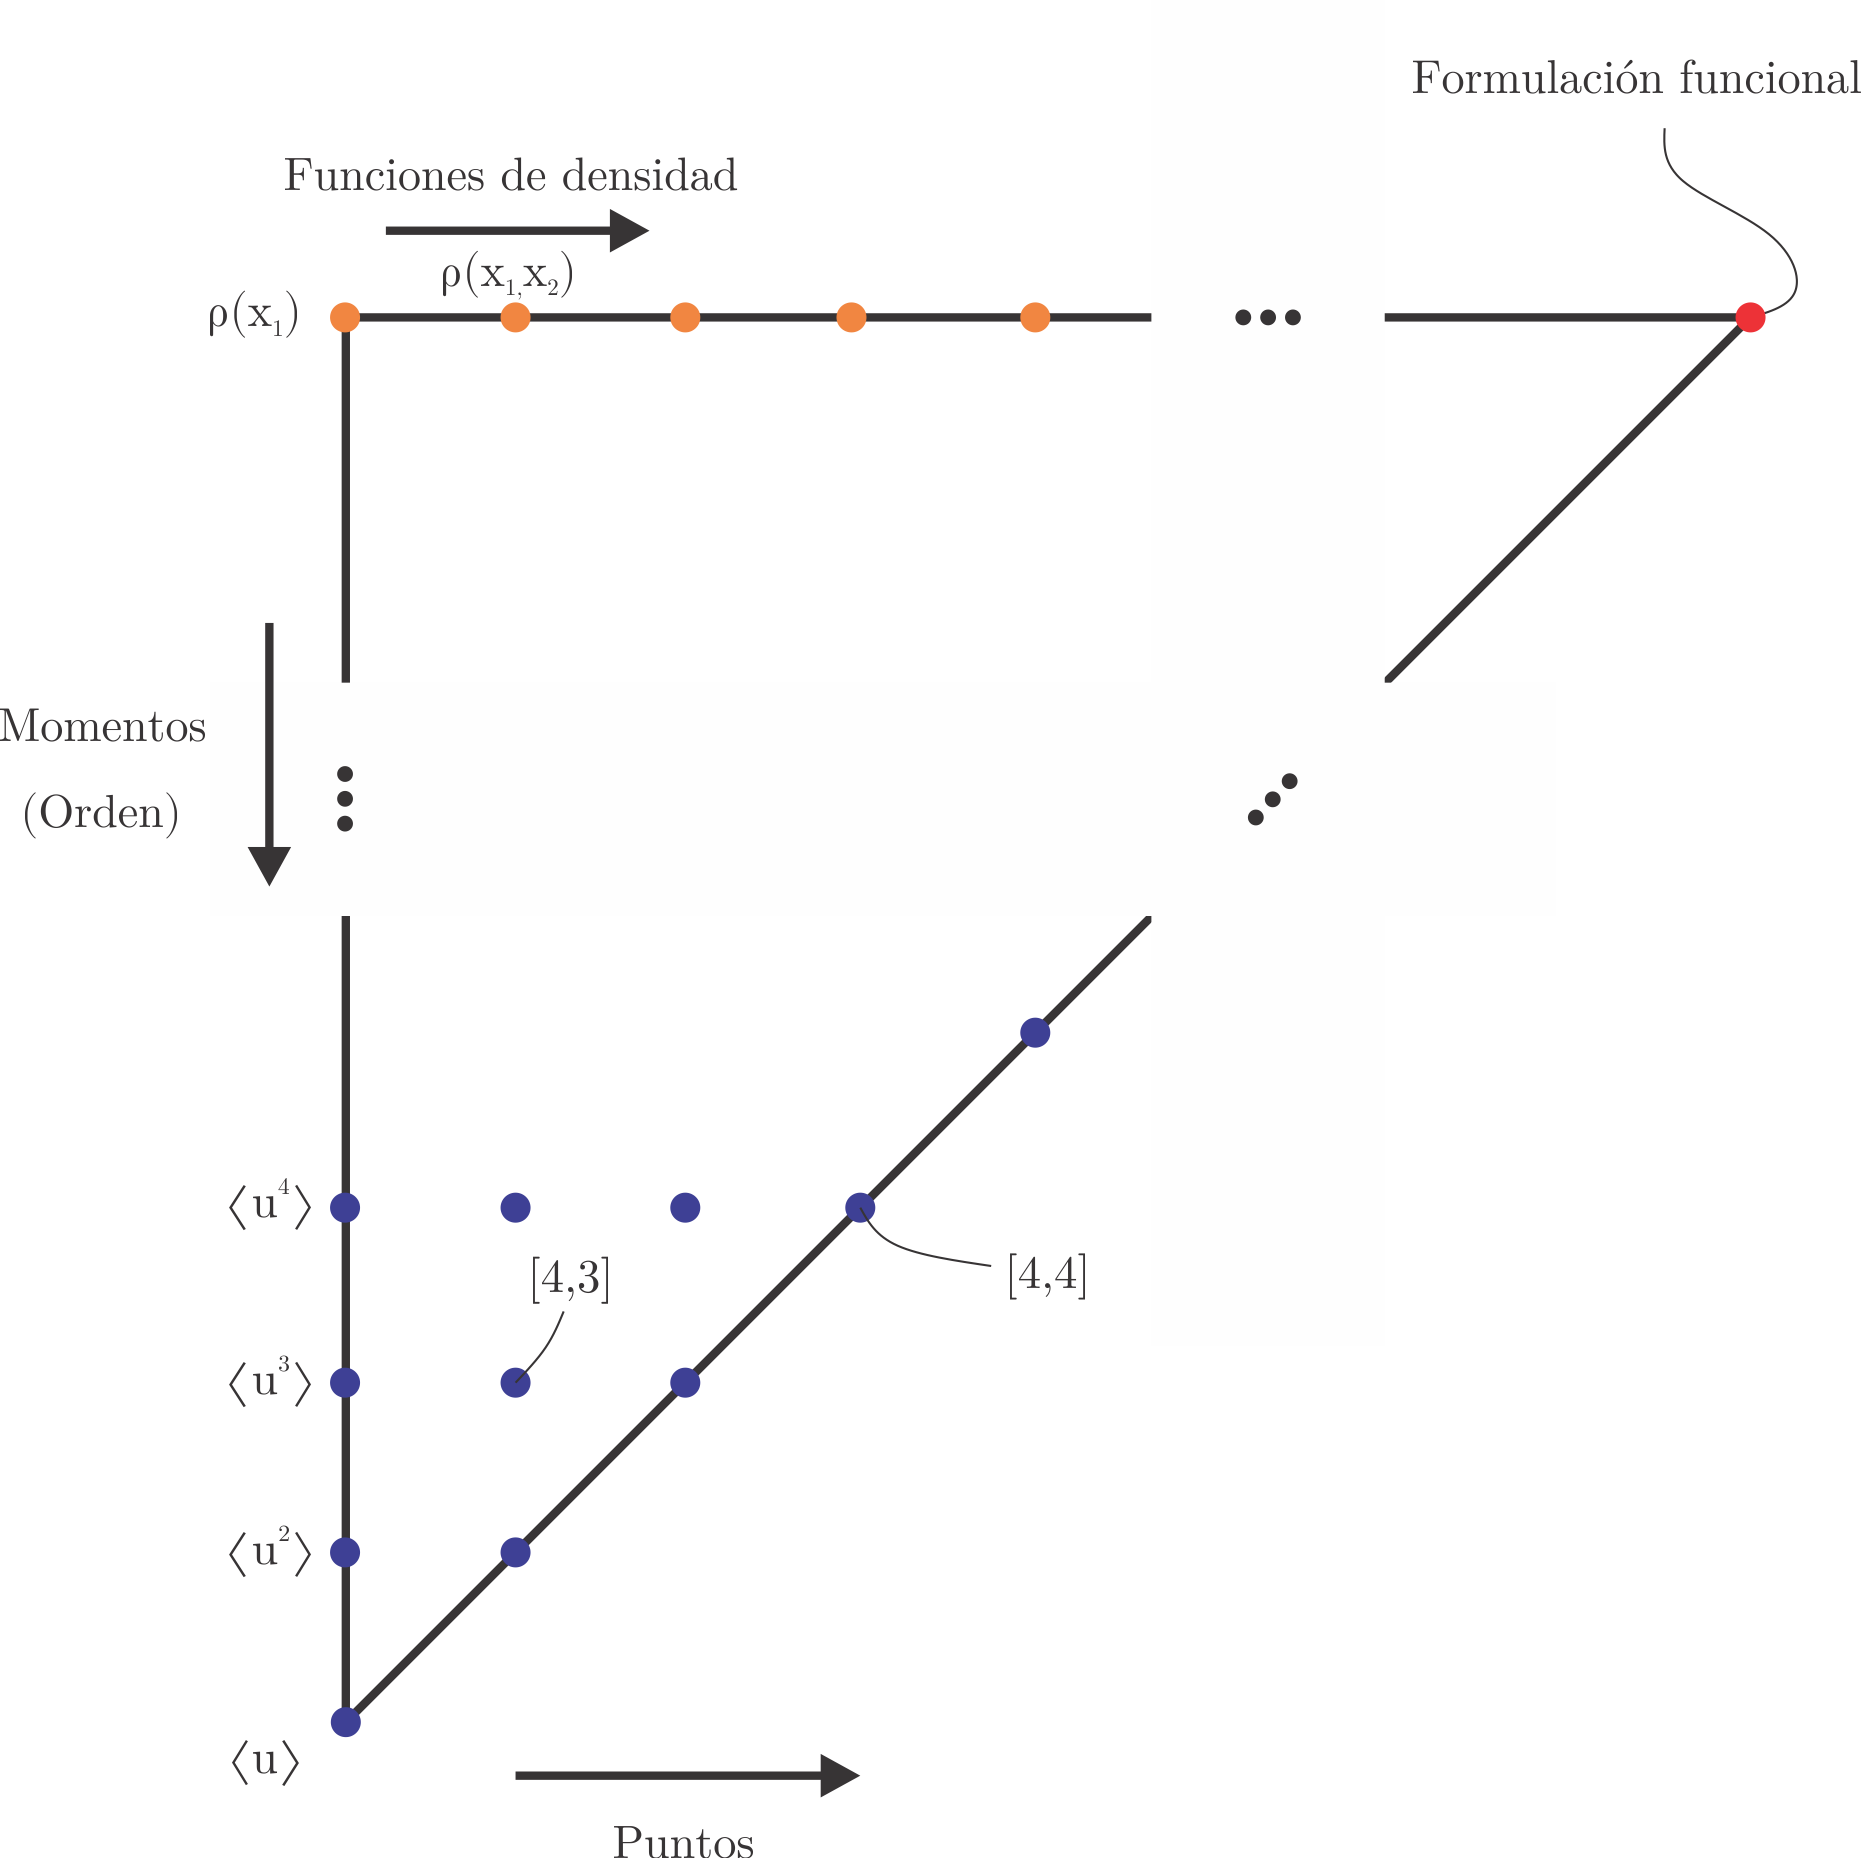
\includegraphics[scale=0.87]{jerarquia}
 	\end{center}
 	\caption{Esquema de jerarquías de ecuaciones en el problema de la turbulencia. }
 	\label{fig-jer1}
 \end{figure}

El sentido de la imagen \ref{fig-jer1} es el siguiente: Cada nodo representa un momento o una descripción, a medida que avanzamos en la vertical tenemos momentos de mayor orden, mientras que al avanzar en la horizontal tenemos descripciones de más puntos. En ciertos sentido, la vertical está relacionada con la no-linealidad (acoplamiento de momentos de distinto orden) y la horizontal está relacionada con la no-localidad generada por la presión. Una vez llegamos a la parte superior del esquema tenemos las funciones de densidad, dado que obteniendo una solución para la función de densidad podemos obtener todos los momentos de la misma cantidad de puntos de la función. Mientras que en la esquina superior derecha tenemos la formulación funcional, que en un sentido es como considerar la densidad en un continuo de puntos (como se describió en la sección de estadística). 


\subsection{Jerarquía de Friedmann-Keller}

Esta jerarquía es la de los momentos, su primera ecuación es usualmente llamada la ecuación RANS (\textit{Reynolds Averaged Navier-Stokes}) para el primer momento de la velocidad. Su derivación es muy simple, consideremos la ecuación de N-S,

\begin{equation*}
	\partial_t u_i + u_j \partial_j u_i =-\frac{1}{\rho}\partial_i p +\nu \partial_j\partial_j u_i
\end{equation*}

Ahora promediemos (promedio de ensamble) estas ecuación, sabemos de las propiedades del promedio (a veces llamadas condiciones de Reynolds) que este conmuta con las derivadas parciales, por lo que de inmediato consideramos esto. Llegamos a,

\begin{equation*}
	\partial_t \langle u_i \rangle + \langle u_j \partial_j u_i \rangle = -\frac{1}{\rho}\partial_i \langle p \rangle +\nu  \partial_j\partial_j \langle u_i \rangle
\end{equation*}


El término que más nos complica es justamente el no-lineal, desarrollandolo,

\begin{align*}
	\langle u_j \partial_j u_i \rangle &= \langle  \partial_j (u_j u_i) \rangle \\
	&=\langle  \partial_j (\langle u_j \rangle + u'_j)(\langle u_i \rangle + u'_i) \rangle\\
	&=\partial_j \langle \langle u_j \rangle \langle u_i \rangle + \langle u_j \rangle u'_i + u'_j\langle u_i \rangle +u'_ju'_i \rangle\\
	&=\partial_j(\langle u_j \rangle \langle u_i \rangle) +\partial_j (\langle u_j \rangle \langle u'_i\rangle ) +\partial_j (\langle u'_j \rangle \langle u_i\rangle ) +\partial_j \langle u'_ju'_i \rangle\\
	&=\langle u_j \rangle \partial_j \langle u_i \rangle+\partial_j \langle u'_ju'_i \rangle
\end{align*}
Donde se usa la incompresibilidad, las propiedades del promedio y el hecho de que el promedio de la fluctuación es cero. Finalmente llegamos a la siguiente ecuación para el primer momento de la velocidad,

\begin{equation}
	\partial_t \langle u_i \rangle + \langle u_j \rangle \partial_j \langle u_i \rangle+\partial_j \langle u'_ju'_i \rangle = -\frac{1}{\rho}\partial_i \langle p \rangle +\nu  \partial_j\partial_j \langle u_i \rangle
\end{equation}

Vemos claramente un acoplamiento entre el primer y segundo momento debido a la presencia del término $\langle u'_ju'_i \rangle$, este tensor de correlación de segundo orden usualmente es llamado tensor de esfuerzos de Reynolds. El problema es que al intentar obtener una ecuación para la correlación de segundo orden vemos que esta depende de la correlación de tercer orden, y así infinitamente. Para poder cortar la jerarquía de ecuaciones en algun momento y resolver el problema se debe recurrir a distintos cierres de la jerarquía.  \\

La ecuación para la correlación de segundo orden es la de Karman-Howarth pero sin asumir isotropía/homogeneidad, es decir, en su caso más general,  

\begin{equation}
	\partial_t\langle v_iv_j' \rangle+\partial_k\langle v_kv_iv_j'\rangle+\partial_k'\langle v_k'v_j'v_i\rangle=-\frac{1}{\rho}(\langle v_j'\partial_i p \rangle+\langle v_i\partial_j' p \rangle )+ \nu (\partial_k\partial_k\langle v_i v_j' \rangle+ \partial_k'\partial_k'\langle v_j'v_i \rangle)
\end{equation}

Notemos que en esta ecuación las variables con prima no corresponden a fluctuaciones, sino a la variable (o derivada) con respecto a otra cordenada, dado que es la ecuación para el tensor de correlación en dos puntos. Nuevamente, como dijimos, vemos el acoplamiento a un momento de orden superior. Lo mismo ocurre para los siguientes momentos. \\
La forma más general que he encontrado hasta ahora es la jerarquía de momentos de dos puntos por Hill \parencite{hill2001}. No detallaremos la derivación, pero la ecuación está dada por,

\begin{equation}
	\partial_t \vb{D}_{N}+\vb{\grad}_x\cdot \vb{F}_{N+1}+\vb{\grad}_r\cdot\vb{D}_{N+1}=-\vb{T}_N+2\nu \left[\left(\grad^2_r+\frac{1}{4}\grad^2_x \right)\vb{D}_N -\vb{E}_N\right]
\end{equation} 

Donde los subindices en el gradiente indican las variables con respecto a las cuales se toma la derivada, recordemos que son las correlaciones de dos puntos por lo que $\vb{x}=\frac{\vb{x_1}+\vb{x}_2}{2}$ y $\vb{r}=\vb{x}_1-\vb{x}_2$. Las cantidades de la ecuación están dadas por,

\begin{align*}
	\vb{D}_{N+1}&=\langle u_nu_j...u_i\rangle\\
	\vb{T}_N&=\langle\left\{u_j...u_lP_i\right\}\rangle\\
	\vb{F}_{N+1}&=\langle U_n u_j...u_i\rangle\\
	\vb{E}_N&=\langle\left\{u_k...u_le_{ij}\right\}\rangle
\end{align*}
Donde $U_n=\frac{u_n(\vb{x_1})+u_n(\vb{x_2})}{2}$, los brackets $\{\}$ indican una suma de términos tal que es simétrica bajo la permutación de un par de indices y $e_{ij}=(\partial_{x_1}u_i)(\partial_{x_1}u_j)+(\partial_{x_2}u_i)(\partial_{x_2}u_j)$. Para más detalles sobre esta jerarquía se puede revisar la investigación citada anteriormente. 


\subsection{Jerarquías de Lundgren-Monin-Novikov}

Esta jerarquía de ecuaciones es la que nos entrega las ecuaciones más importantes para nuestros propositos. Dado que a partir de las ecuaciones para las densidades podemos investigar la entropía del sistema. Originalmente el sistema fue derivado por Lundgren \parencite{lundgren1967} para la velocidad, luego Monin y Novikov obtuvieron las pdf para la vorticidad, una review de estas jerarquías fue realizada por Friedrich \parencite{friedrich2012}. \\

Primero vamos a estudiar la jerarquía de Lundgren, para esto considera el operator de Perron-Frobenius $\delta\left[\vb{u}(\vb{x},t)-\hat{\mathcal{L}}_t \vb{u}_0\right]$, donde $\hat{\mathcal{L}}_t$ es la regla de evolución temporal. El operator transporta la densidad desde una condición inicial  $\vb{u}_0$ en el tiempo $0$ a la densidad en $t$ según,

 \begin{equation*}
 	\rho(\vb{u},\vb{x},t)=\int \delta\left[\vb{u}(\vb{x},t)-\hat{\mathcal{L}}_t \vb{u}_0\right] \rho(\vb{u}_0,\vb{x},0) d\vb{u}_0 = \langle\delta\left[\vb{u}(\vb{x},t)-\hat{\mathcal{L}}_t \vb{u}_0\right]\rangle
 \end{equation*}

Es importante notar que el promedio es realizado sobre las condiciones iniciales en todo el espacio de fase, es decir, es una integración funcional. Llamando $\vb{v}=\hat{\mathcal{L}}_t \vb{u}_0$ entonces tenemos,

\begin{equation*}
	\rho(\vb{u},\vb{x},t)=\langle\delta\left[\vb{u}(\vb{x},t)-\vb{v}\right]\rangle
\end{equation*}
De la misma forma la función de densidad de dos puntos está dada por,

\begin{equation*}
	\rho_2(\vb{v}_1,\vb{x}_1,\vb{v}_2,\vb{x}_2,t)=\langle\delta\left[\vb{u}_1(\vb{x}_1,t)-\vb{v}_1\right]\delta\left[\vb{u}_2(\vb{x}_2,t)-\vb{v}_2\right]\rangle
\end{equation*}

Consideremos por el momento solo una componente de $\vb{u}$, derivando con respecto al tiempo (teniendo en cuenta que la función delta es una función de $\vb{v}$),

\begin{equation*}
	\partial_t \rho(v_i,\vb{x},t)=\langle \partial_t \delta\left[u_i(\vb{x},t)-v_i\right] \rangle = -\langle \partial_{v_i} \delta\left[u_i(\vb{x},t)-v_i\right] \partial_t u_i \rangle
\end{equation*}

Pero sabemos cual es la evolución temporal de $u_i$, la ecuación de N-S, por lo tanto tenemos (abreviando la notación para que el proceso no sea tan engorroso),

\begin{equation*}
	\partial_t \rho(v_i)=-\langle \partial_{v_i} \delta\left[u_i-v_i\right] \left\{ -u_j \partial_j u_i -\frac{1}{\rho}\partial_i p +\nu \partial_j\partial_j u_i\right\} \rangle
\end{equation*}

 Distribuyendo en la ecuación obtenemos,
 
 \begin{equation*}
 	\partial_t \rho(v_i)=\underbrace{\langle \partial_{v_i} \delta\left[u_i-v_i\right]u_j \partial_j u_i\rangle}_{I} +\frac{1}{\rho} \underbrace{\langle \partial_{v_i} \delta\left[u_i-v_i\right]\partial_i p \rangle}_{II} -\nu \underbrace{\langle \partial_{v_i} \delta\left[u_i-v_i\right]\partial_j\partial_j u_i \rangle}_{III}
 \end{equation*}

Ahora estudiamos todos los términos, empezando por $I$. Consideremos la derivada con respecto a alguna coordenada temporal del operator, de la misma forma que en el caso de la derivada temporal, 

\begin{align*}
	\langle \partial_{x_j} \delta\left[u_i-v_i\right] \rangle = -\langle \partial_{v_i} \delta\left[u_i-v_i\right] \partial_{x_j} u_i \rangle
\end{align*}

Comparando esto con el término $I$ vemos que,

\begin{align*}
	\langle \partial_{v_i} \delta\left[u_i-v_i\right]u_j \partial_{x_j} u_i\rangle&=-\langle u_j\partial_{x_j}\delta(u_i-v_i) \rangle\\
	&=-\langle \partial_{x_j} \left[u_j\delta(u_i-v_i)\right] \rangle\\
	&=-\partial_{x_j} \langle u_j\delta(u_i-v_i) \rangle
\end{align*}
Donde se uso el hecho de que el flujo es incompresible. Ahora consideremos la siguiente propiedad de la función delta,

\begin{equation*}
	\int \delta(x-a)f(x)dx=f(a)=\int \delta(x-a)f(a) dx
\end{equation*}
por lo tanto dentro del promedio hacemos el siguiente cambio,

\begin{equation*}
	-\partial_{x_j} \langle u_j\delta(u_i-v_i) \rangle=-\partial_{x_j} \langle v_j\delta(u_i-v_i) \rangle
\end{equation*}
Por lo tanto podemos sacar $v_j$ del promedio,

\begin{equation*}
	-\partial_{x_j} \langle v_j\delta(u_i-v_i) \rangle=-\partial_{x_j} v_j\langle\delta(u_i-v_i) \rangle=-v_j\partial_{x_j} \langle\delta(u_i-v_i) \rangle=-v_j\partial_{x_j} \rho(v_i)
\end{equation*}

Para el segundo término ($II$) podemos escribir la presión en términos de la velocidad (utilizando la función de Green) como,

\begin{equation*}
	p=\frac{1}{4\pi}\int \frac{\partial_{x'_j} u'_k\partial_{x'_k} u'_j}{\abs{\vb{x}-\vb{x'}}}d\vb{x'}
\end{equation*}
Por lo tanto tenemos,
\begin{align*}
	\langle \partial_{v_i} \delta\left[u_i-v_i\right]\partial_{x_i} p \rangle&=\frac{1}{4\pi}\langle \partial_{x_i} \left[\int \frac{\partial_{x'_j} u'_k\partial_{x'_k} u'_j}{\abs{\vb{x}-\vb{x'}}}d\vb{x'} \right]  \partial_{v_i}\delta(u_i-v_i)\rangle\\
	&=-\frac{1}{4\pi}\partial_{v_i}\langle \partial_{x_i} \left[\int \frac{\partial_{x'_j} u'_k\partial_{x'_k} u'_j}{\abs{\vb{x}-\vb{x'}}}d\vb{x'}\right]   \delta(u_i-v_i)\rangle
\end{align*}

Primero notamos que podemos agregar un término de la forma $\int  \delta(u_l'-v_l') dv_l'$ dentro de la integral, dado que el valor de este es $1$, luego tenemos,

\begin{align*}
	&-\frac{1}{4\pi}\partial_{v_i}\langle \partial_{x_i} \left[\int \frac{\partial_{x'_j} u'_k\partial_{x'_k} u'_j}{\abs{\vb{x}-\vb{x'}}}d\vb{x'}\right]   \delta(u_i-v_i)\rangle\\
	=&-\frac{1}{4\pi}\partial_{v_i}\langle \partial_{x_i} \left[\int \frac{\partial_{x'_j} u'_k\partial_{x'_k} u'_j}{\abs{\vb{x}-\vb{x'}}} \int  \delta(u_l'-v_l') dv_l' d\vb{x'}\right]   \delta(u_i-v_i)\rangle\\
	=&-\frac{1}{4\pi}\partial_{v_i}\int \partial_{x_i}\left(\frac{1}{\abs{\vb{x}-\vb{x'}}}\right) \langle \partial_{x'_j} u'_k\partial_{x'_k} u'_j \delta(u_l'-v_l')\delta(u_i-v_i)\rangle dv_l' d\vb{x'}\\
	=&-\frac{1}{4\pi}\partial_{v_i}\int \partial_{x_i}\left(\frac{1}{\abs{\vb{x}-\vb{x'}}}\right) \langle \partial_{x'_j} v'_k\partial_{x'_k} v'_j \delta(u_l'-v_l')\delta(u_i-v_i)\rangle dv_l' d\vb{x'}\\
	=&-\frac{1}{4\pi}\partial_{v_i}\int \partial_{x_i}\left(\frac{1}{\abs{\vb{x}-\vb{x'}}}\right)  \partial_{x'_j} v'_k\partial_{x'_k} v'_j \langle \delta(u_l'-v_l')\delta(u_i-v_i)\rangle dv_l' d\vb{x'}\\
	=&-\frac{1}{4\pi}\partial_{v_i}\int \partial_{x_i}\left(\frac{1}{\abs{\vb{x}-\vb{x'}}}\right) \partial_{x'_j} v'_k\partial_{x'_k} v'_j \rho(v_i,v'_l) dv_l' d\vb{x'}\\
\end{align*} 

El punto importante de este termino es que, como vemos, debido a la no-localidad impuesta por el término correspondiente a la presión en turbulencia incompresible, tenemos que la evolución temporal de la función de densidad de un punto depende también de la función de dos puntos. Para el término $III$ tenemos, 

\begin{align*}
	\langle \partial_{v_i} \delta\left[u_i-v_i\right]\partial_j\partial_j u_i \rangle&=\nu \partial_{v_i} \langle \partial_j\partial_j u_i  \delta (u_i-v_i) \rangle\\
	&=\nu \partial_{v_i} \partial_j\partial_j \langle  u_i  \delta (u_i-v_i) \rangle\\
	&=\nu \partial_{v_i} \lim_{x\to x'}\partial_{x_j'}\partial_{x_j'} \langle  u'_i  \delta (u_i-v_i) \rangle\\
	&=\nu \partial_{v_i} \lim_{x\to x'}\partial_{x_j'}\partial_{x_j'} \int \langle  u'_i  \delta(u_l'-v_l')   \delta (u_i-v_i) \rangle dv_l'\\
	&=\nu \partial_{v_i} \lim_{x\to x'}\partial_{x_j'}\partial_{x_j'} \int \langle  v'_i  \delta(u_l'-v_l')   \delta (u_i-v_i) \rangle dv_l'\\
	&=\nu \partial_{v_i} \lim_{x\to x'}\partial_{x_j'}\partial_{x_j'} \int v'_i \rho(v,v') dv_l'\\
\end{align*}

Vemos que el término viscoso también acopla la ecuación de evolución con la de siguiente orden. Finalmente, usando notación vectorial la ecuación de evolución para la función de densidad es,

\begin{equation*}
	\partial_t \rho_1 +\vb{v}\cdot \partial_{\vb{x}}\rho_1=\frac{1}{\rho}\frac{1}{4\pi}\partial_{\vb{v}}\int \partial_{\vb{x}}\left(\frac{1}{\abs{\vb{x}-\vb{x}'}}\right)\cdot\left(\vb{v}'\cdot\partial_{\vb{x}'}\right)^2\rho_2d\vb{x}'d\vb{v}'-\nu\lim_{\vb{x}\to \vb{x}'}\partial_{\vb{x}'}\cdot\partial_{\vb{x}'}\int \vb{v}'\rho_2 d\vb{v}'
\end{equation*}
Donde $\rho_2$ y $\rho_1$ se refieren a las densidad de dos y un punto respectivamente. Se puede escribir una ecuación genérica para las pdf de todos los ordenes tal como lo hace \parencite{friedrich2012}, 

\begin{align*}
	\left(\partial_t +\sum_{i=1}^N \vb{u}_i \grad{}_{\vb{x}_i}\right)\rho_N=&-\sum_{i=1}^N\grad{}_{\vb{u}_j}\cdot\int \vb{K}(\vb{x}_j-\vb{x}')(\vb{u}'\cdot\grad{}_{\vb{x}'})^2 \rho_{N+1} d\vb{u'} d\vb{x}'\\
	&-\nu\sum_{j=1}^{N}\grad{}_{\vb{u}_j}\cdot\int\delta(\vb{x}_j-\vb{x}')\vb{u}'\nabla^2_{\vb{x}'}\rho_{N+1}d\vb{u}'
\end{align*}

También existe una formulación para la vorticidad dada por,


\begin{align*}
	&\partial_t\rho_N +\sum_{i=1}^N \grad{}_{\vb{x}_i}\cdot \int  \vb{\omega}' \times \vb{K}(\vb{x}_i-\vb{x}')\rho_{N+1}  d\vb{\omega}' d\vb{x}' \\
	&=-\sum_{i=1}^N\grad{}_{\vb{\omega}_j}\cdot\int \vb{\omega}'\times\vb{K}(\vb{x}_j-\vb{x}')\vb{\omega}\cdot\grad{}_{\vb{x}'} \rho_{N+1} d\vb{\omega'} d\vb{x}'\\
	&-\sum_{i=1}^{N}\grad{}_{\vb{\omega}_i}\cdot\int\vb{\omega}'\delta(\vb{x}_i-\vb{x}')\nabla^2_{\vb{x}'}\rho_{N+1}d\vb{u}'
\end{align*}

\subsection{Formulación en términos del funcional de Hopf}

La forma más compacta de plantear el problema estadístico de la turbulencia es en términos del funcional de Hopf \parencite{hopf1952}, un análisis muy detallado de este enfoque puede ser estudiado en el libro de Monin y Yaglom \parencite{monin1976}. Como ya introdujimos anteriormente, el funcional característico tiene toda la información sobre la estadística de un proceso aleatorio (también de un campo, solo tenemos que agregar las dimensiones espaciales al problema), el funcional característico espacio-temporal está dado por,

\begin{equation*}
	\Psi[\bm{\theta}(\vb{x},t)]=\langle e^{i\int \bm{\theta}(\vb{x},t)\cdot\vb{u}(\vb{x},t) d\vb{x}} \rangle
\end{equation*}
Podemos ver que si seleccionamos $\bm{\theta}(\vb{x},t)=\sum_{k=1}^N \bm{\theta}_k \delta(\vb{x}-\vb{x}_k)\delta(t-t_k)$ entonces tenemos,

\begin{equation}
	\int \bm{\theta}(\vb{x},t)\cdot\vb{u}(\vb{x},t) d\vb{x}=\sum_{k=1}^N \bm{\theta}_k \cdot \vb{u}(\vb{x}_k,t_k)
\end{equation}

y el funcional se transforma en,

\begin{equation*}
	\Psi[\bm{\theta}(\vb{x},t)]=\langle e^{i\sum_{k=1}^N \bm{\theta}_k \cdot \vb{u}(\vb{x}_k,t_k)}\rangle
\end{equation*}
Esta es simplemente la función característica de $N$ puntos espaciales y temporales, por lo que vemos que a partir del funcional característico podemos obtener información sobre cualquier pdf de la jerarquía de Lundgren, y dado que a partir de estas últimas podemos obtener todos los momentos de la jerarquía de Friemann-Keller, entonces el funcional nos da una descripción estadística completa del problema. Entonces tenemos que realizarnos la siguiente pregunta, 'Que ecuacion obedece la evolución temporal del funcional?'. Para esto debemos estudiar la derivada temporal de $\Psi$, actualmente lo haremos solo con la versión espacial del funcional, es decir uno de la forma $\Psi[\bm{\theta}(\vb{x}),t]$, este no tiene información sobre la estructura temporal del campo dado que solo podemos obtener funciones de densidad de un punto en el tiempo, sin embargo contiene información completa sobre la estructura espacial \parencite{monin1976}. El funcional tiene la forma,

\begin{equation*}
	\Psi[\bm{\theta}(\vb{x}),t]=\langle e^{i\int \bm{\theta}(\vb{x})\cdot\vb{u}(\vb{x},t) d\vb{x}} \rangle
\end{equation*}

Tomando la derivada temporal,

\begin{align*}
	\partial_t\Psi[\bm{\theta}(\vb{x}),t]&=\langle \partial_t e^{i\int \bm{\theta}(\vb{x})\cdot\vb{u}(\vb{x},t) d\vb{x}} \rangle\\
	&=i\langle \partial_t\left[\int \bm{\theta}(\vb{x}')\cdot\vb{u}(\vb{x}',t) d\vb{x}'\right] e^{i\int \bm{\theta}(\vb{x})\cdot\vb{u}(\vb{x},t) d\vb{x}} \rangle\\
	&=i\int \bm{\theta}(\vb{x}')\cdot\langle \partial_t \vb{u}(\vb{x}',t)e^{i\int \bm{\theta}(\vb{x})\cdot\vb{u}(\vb{x},t) d\vb{x}} \rangle d\vb{x}'\\
\end{align*}

Ahora reemplazamos la ecuación de N-S en la última ecuación,

\begin{align*}
	i\int \bm{\theta}(\vb{x}')\cdot\langle \partial_t \vb{u}(\vb{x}',t)e^{i\int \bm{\theta}(\vb{x})\cdot\vb{u}(\vb{x},t) d\vb{x}} \rangle d\vb{x}'=&i\int \bm{\theta}(\vb{x}')\cdot\langle ( -\vb{u}(\vb{x}',t)\cdot\grad{} \vb{u}(\vb{x}',t)\\
	&-\frac{1}{\rho}\grad{}p(\vb{x}',t) +\nu\grad{}^2\vb{u}(\vb{x}',t) )e^{i\int \bm{\theta}(\vb{x})\cdot\vb{u}(\vb{x},t) d\vb{x}} \rangle d\vb{x}'
\end{align*}

Para reducir esta expresión debemos recurrir a la derivada funcional,

\begin{align*}
	\frac{\delta \Psi}{\delta \theta_j (\vb{x''})}&=\langle \frac{\delta}{\delta \theta_j (\vb{x''})}e^{i\int \bm{\theta}(\vb{x})\cdot\vb{u}(\vb{x},t) d\vb{x}} \rangle\\
	&=i\int \langle \delta(\vb{x}'-\vb{x}'')u_j(\vb{x}',t) e^{i\int \bm{\theta}(\vb{x})\cdot\vb{u}(\vb{x},t) d\vb{x}} \rangle d\vb{x}'\\
	&=i\langle u_j(\vb{x}'',t) e^{i\int \bm{\theta}(\vb{x})\cdot\vb{u}(\vb{x},t) d\vb{x}} \rangle \\
\end{align*}

De la misma forma se puede obtener una expresión para la segunda derivada funcional,

\begin{equation*}
	\frac{\delta \Psi}{\delta \theta_l (\vb{x''})\theta_j (\vb{x''})}=-\langle u_l(\vb{x}'',t) u_j(\vb{x}'',t) e^{i\int \bm{\theta}(\vb{x})\cdot\vb{u}(\vb{x},t) d\vb{x}} \rangle
\end{equation*}

Ahora podemos analizar los distintos términos, para el no-lineal tenemos,

\begin{align*}
	-\langle \vb{u}(\vb{x}',t)\cdot\grad{} \vb{u}(\vb{x}',t)e^{i\int \bm{\theta}(\vb{x})\cdot\vb{u}(\vb{x},t) d\vb{x}} \rangle &=-\langle u_j(\vb{x}',t)\partial'_j u_l(\vb{x}',t)e^{i\int \bm{\theta}(\vb{x})\cdot\vb{u}(\vb{x},t) d\vb{x}} \rangle\\ 
	&=-\partial'_j \langle u_j(\vb{x}',t) u_l(\vb{x}',t)e^{i\int \bm{\theta}(\vb{x})\cdot\vb{u}(\vb{x},t) d\vb{x}} \rangle\\ 
	&=\partial'_j  \frac{\delta}{\delta \theta_l (\vb{x'})\theta_j (\vb{x'})} \langle e^{i\int \bm{\theta}(\vb{x})\cdot\vb{u}(\vb{x},t) d\vb{x}} \rangle\\
	&=\partial'_j  \frac{\delta}{\delta \theta_l (\vb{x'})\theta_j (\vb{x'})} \Psi [\bm{\Theta}(\vb{x}),t]
\end{align*}

Para el término de la presión (reescribiendola en términos de la función de Green),

\begin{align*}
	\langle p(\vb{x}') e^{i\int \bm{\theta}(\vb{x})\cdot\vb{u}(\vb{x},t) d\vb{x}} \rangle&=-\frac{1}{4\pi} \frac{1}{\abs{\vb{x}-\vb{x}''}} \langle \partial''_l \partial''_j(u_l(\vb{x}'',t)u_j(\vb{x}'',t)) e^{i\int \bm{\theta}(\vb{x})\cdot\vb{u}(\vb{x},t) d\vb{x}} \rangle d\vb{x}''\\
	&=\frac{1}{4\pi} \frac{1}{\abs{\vb{x}-\vb{x}''}} \partial''_l\partial''_j \frac{\delta }{\delta \theta_l (\vb{x''})\theta_j (\vb{x''})}\Psi [\bm{\Theta}(\vb{x}),t] d\vb{x}''\\
\end{align*}

Y para el término de la disipación, 

\begin{align*}
	\nu \langle \grad{}^2 \vb{u}(\vb{x}') e^{i\int \bm{\theta}(\vb{x})\cdot\vb{u}(\vb{x},t) d\vb{x}}\rangle&= \nu  \grad{}^2 \langle u_j(\vb{x}') e^{i\int \bm{\theta}(\vb{x})\cdot\vb{u}(\vb{x},t) d\vb{x}}\rangle\\
	&=-i\nu  \grad{}^2 \frac{\delta}{\delta\theta_j(\vb{x}')}\langle e^{i\int \bm{\theta}(\vb{x})\cdot\vb{u}(\vb{x},t) d\vb{x}}\rangle\\
	&=-i\nu  \grad{}^2 \frac{\delta}{\delta\theta_j(\vb{x}')}\Psi [\bm{\Theta}(\vb{x}),t]\\
\end{align*}

Por lo que finalmente, uniendo todos los términos llegamos a la ecuación para la evolución temporal del funcional de Hopf,

\begin{align*}
	\partial_t \Psi [\bm{\Theta}(\vb{x}),t] = \int \alpha_k(\vb{x}')\bigg[i\partial'_j \frac{\delta^2}{\delta\theta_j(\vb{x}') \delta\theta_k(\vb{x}')}& +\frac{1}{4\pi}\partial_k'\int \frac{1}{\abs{(\vb{x}'-\vb{x}'')}}\partial''_l\partial''_j \frac{\delta^2}{\delta\theta_l(\vb{x}'') \delta\theta_j(\vb{x}'') } \\&+\nu\grad{}^2 \frac{\delta}{\delta\theta_k(\vb{x}')} \bigg] \Psi [\bm{\Theta}(\vb{x}),t]
\end{align*}

Lo interesante es que debido a la incompresibilidada existe una invarianza de la forma $\alpha_k(\vb{x}) \to \alpha_k(\vb{x})+\partial_k\phi(\vb{x})$ y esto se puede usar para reemplazar el término de la presión \parencite{friedrich2020}, llegando a una ecuación de la forma, 


\begin{equation*}
	\partial_t \Psi [\bm{\Theta}(\vb{x}),t] = \int \alpha'_k(\vb{x}')\bigg[i\partial'_j \frac{\delta^2}{\delta\theta_j(\vb{x}') \delta\theta_k(\vb{x}')}  +\nu\grad{}^2 \frac{\delta}{\delta\theta_k(\vb{x}')} \bigg] \Psi [\bm{\Theta}(\vb{x}),t]
\end{equation*}

Una de las propiedades más útiles de esta ecuación es que es lineal, y esto puede hacernos creer que el problema está solucionado, sin embargo aún no existen los métodos para resolver ecuaciones funcionales lineales, por lo que actualmente aún no se puede extraer mucha información útil a partir de esta.




\pagebreak

\section{Estabilidad hidrodinámica}

\subsection{La ecuación de Orr-Sommerfeld}
Uno de los aspectos más importantes en el estudio de los flujos turbulentos es la transición. Como se transforma un flujo laminar a uno turbulento? Y no es una pregunta trivial, pues aun más enigmático es el hecho de que, al agregar los efectos viscosos un flujo que de otra manera sería estable, se vuelve inestable (contrario a la intuición, dado que a priori uno pensaría que al agregar el efecto de las viscosidad, ésta funcionaria como un amortiguamiento y por lo tanto haría el flujo más estable).\\
A continuación presentaremos los aspectos más básicos de la teoría de estabilidad hidrodinámica, existen diversos libres donde se puede consultar la teoría más a fondo \parencite{criminale2018,schlichting2016,chandrasekhar2013,yaglom2012}. Para comenzar a estudiar éste aspecto primero debemos derivar una ecuación para las perturbaciónes. Consideremos un flujo paralelo (puede ser un flujo de corte como un canal) tal que $\vb{u}=\vb{U}+\vb{u}'$, entonces las ecuaciones de Navier-Stokes son,

\begin{equation}
	\partial_t U_i+u'_i+\left[\partial_{j}(U_j+u'_j)\right](U_i+u'_i)=-\partial_i p + \partial_j\partial_{j} (U_i+u'_i)
\end{equation}  


\begin{figure}[H]
	\begin{center}
		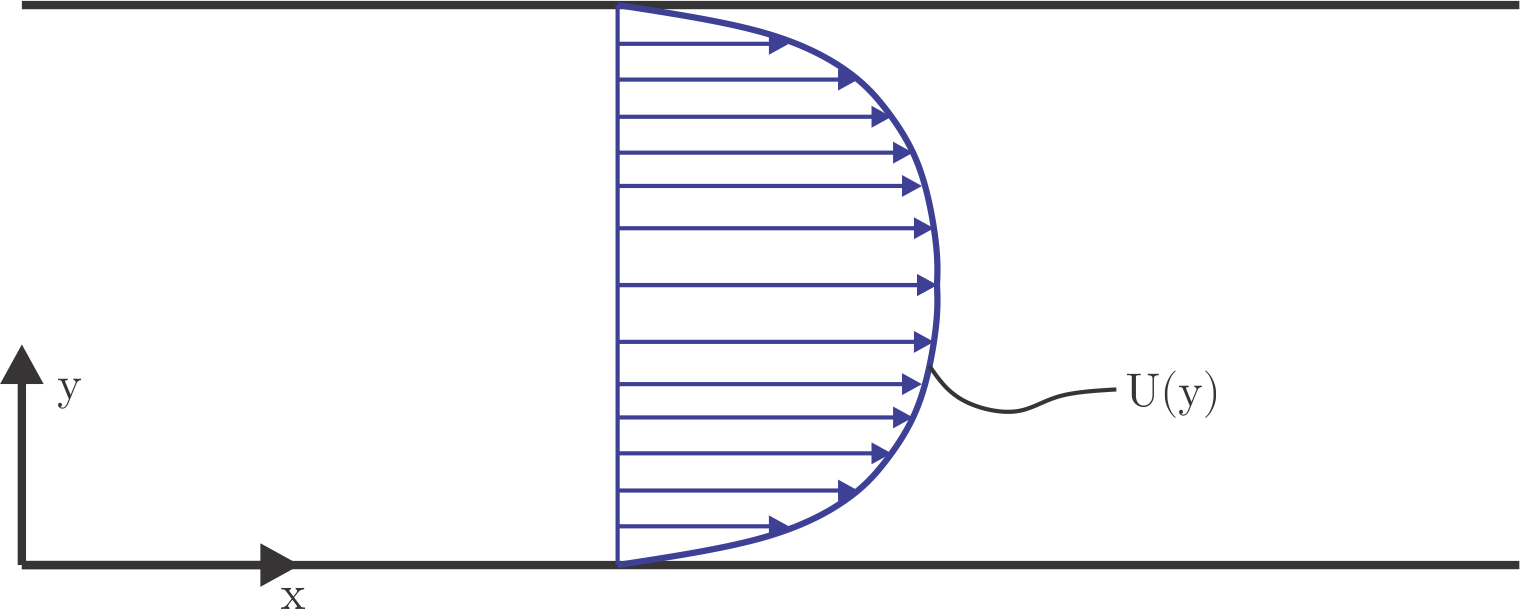
\includegraphics[scale=1]{estabilidad1}
	\end{center}
	\caption{Perfil de velocidad en un canal laminar, observamos que la velocidad solo tiene componente en $x$ y gradiente en $y$.}
	\label{fig-stability1}
\end{figure}


Dado que consideramos un flujo paralelo, podemos orientar convenientemente el flujo medio $\vb{U}=U(y)\hat{i}$ de tal forma que tenga solo componente en $x$ (como es mostrado en la figura), además también agregamos una perturbación a la presión $p=P+p'$.  Ahora haremos referencia al teorema de Squire \parencite{squire1933}, según el cual (como explica Criminale \parencite{criminale2018}) para cada perturbación tridimensional corresponde una bidimensional más inestable, por lo cual basta con analizar un flujo 2D (esto es solo válido para teoría de estabilidad lineal). Por lo tanto para la ecuación de la componente $x$ (considerando $u_x=U+u'$, $u_y=v$) tenemos,

\begin{equation*}
	\partial_t U +\partial_t u' +(U+u')\partial_x (U+u') + v'\partial_y u'  =-\frac{1}{\rho} \partial_x(P+p')+\nu(\partial_x^2 + \partial_y^2 )(U+u')
\end{equation*}

Ahora, dado que consideramos perturbaciones pequeñas, descartarmos los términos de segundo orden en las perturbaciones. Además el flujo base se considera estacionario, por lo que se anula su derivada temporal,

\begin{equation*}
	\partial_t u' +U\partial_x u'  =-\frac{1}{\rho} \partial_x(P+p')+\nu(\partial_x^2 + \partial_y^2 )u' +\nu\partial_y^2 U
\end{equation*}

Para la componente $y$ tenemos la siguiente ecuación,
\begin{equation*}
	\partial_tv' + (U+u')\partial_x v' +v'\partial_y v' = -\frac{1}{\rho} \partial_y(P+p')+\nu (\partial_x^2 +\partial_y^2)v'
\end{equation*}

También sabemos que el flujo base es una solución a las ecuaciones de Navier-Stokes por lo tanto satisface las siguientes relaciones,
\begin{equation*}
	\nu\partial^2_y -\frac{1}{\rho} \partial_P =0 \hspace{0.5cm} -\frac{1}{\rho}\partial_yP=0
\end{equation*}
Y también debe ser incompresible,
\begin{equation*}
	\grad{}\cdot\vb{U}=0\implies \grad{}\cdot \vb{u}'=\partial_xu'+\partial_yv'=0
\end{equation*}
Luego tenemos el siguiente sistema de ecuaciones para la evolución temporal de las perturbaciones lineales sobre el flujo base,


\begin{align*}
	\partial_t u' +U\partial_x u' & =-\frac{1}{\rho} \partial_xp'+\nu(\partial_x^2 + \partial_y^2 )u' \\
		\partial_tv' + U\partial_x v'  &= -\frac{1}{\rho} \partial_yp'+\nu (\partial_x^2 +\partial_y^2)v'\\
	\partial_xu'+\partial_yv'&=0
\end{align*}

Es posible descoplar las ecuaciones para $v'$. Primero derivamos la ecuación de $u'$ con respecto a $y$,

\begin{equation*}
	\partial_t \partial_y u' +\partial_y (U\partial_xu')+\partial_y (v'\partial_y U)=-\frac{1}{\rho}\partial_y\partial_x p' +\nu \partial_y (\partial_x^2 +\partial_y^2)u'
\end{equation*}
Ahora derivamos la ecuación de $v'$ con respecto a $x$,

\begin{equation*}
	\partial_t \partial_xv' +\partial_x(U\partial_x v')=-\frac{1}{\rho}\partial_x\partial_y +\nu\partial_x(\partial_x^2 +\partial_y^2)v'
\end{equation*}

Si restamos ambas ecuaciones observamos que (debido a la conmutatividad de las derivadas parciales) se anulan los términos de la presión, por lo que llegamos a, 

\begin{align*}
	\partial_t(\partial_y u' -\partial_x v') +\partial_y(U\partial_x u')-\partial_x(U\partial_x v')+\partial_y(v'\partial_y U)=\nu(\partial_x^2 +\partial_y^2)(\partial_yu'-\partial_xv')
\end{align*}
Manipulando los siguientes términos,

\begin{align*}
	&\partial_y(U\partial_x u')-\partial_x(U\partial_x v')+\partial_y(v'\partial_y U)\\
	=&\partial_yU\partial_xu'+U\partial_y\partial_xu'+\partial_yv'\partial_yU+v'\partial_y^2U-\partial_xU\partial_xv'-U\partial_x^2v'\\
	=&\partial_yU(\partial_xu'+\partial_yv')+U\partial_x(\partial_yu'-\partial_xv')+v'\partial_y^2U-\partial_xU\partial_xv'\\
	=&U\partial_x(\partial_yu'-\partial_xv')+\partial_y^2 U v'
\end{align*}
Donde en la tercera línea se uso el hecho de que $\partial_xU(y)=0$ y $\partial_xu'+\partial_yv'=0$. Luego llegamos a la siguiente ecuación,

\begin{equation}
	\partial_t(\partial_y u' -\partial_x v') +U\partial_x(\partial_yu'-\partial_xv')+\partial_y^2 U v'=\nu(\partial_x^2 +\partial_y^2)(\partial_yu'-\partial_xv')
	\label{eq.orr1}
\end{equation}
Ahora derivamos esta con respecto a $x$,

\begin{equation*}
	\partial_t(\partial_y \partial_xu' -\partial_x^2 v') +U\partial_x(\partial_y\partial_xu'-\partial_x^2v')+\partial_y^2 U \partial_xv'=\nu(\partial_x^2 +\partial_y^2)(\partial_y\partial_xu'-\partial_x^2v')
\end{equation*}
Usando la incompresibilidad reemplazamos $\partial_xu'=-\partial_y v'$,

\begin{equation*}
	\partial_t(\partial_y^2v' +\partial_x^2 v') +U\partial_x(\partial_y^2v'+\partial_x^2v')-\partial_y^2 U \partial_xv'=\nu(\partial_x^2 +\partial_y^2)(\partial_y^2v'+\partial_x^2v')
\end{equation*}

Finalmente llegamos a la ecuación,
\begin{equation}
	(\partial_t  +U\partial_x)(\partial_y^2 +\partial_x^2) v'+\partial_y^2 U \partial_xv'=\nu(\partial_x^2 +\partial_y^2)(\partial_y^2+\partial_x^2)v'
\end{equation}
O en términos de operadores,

\begin{equation}
	(\partial_t  +U\partial_x)\gradient^2 v'-\partial_y^2 U \partial_xv'=\nu\gradient^4v'
	\label{eq.orr2}
\end{equation}
Donde $\gradient^4=(\partial_x^2 +\partial_y^2)(\partial_y^2+\partial_x^2)$ es el llamado operador biarmónico. La ecuación \ref{eq.orr2} es conocida como ecuación de Orr-Sommerfeld para la velocidad. Más conocida es su formulación para la función de flujo, consideremos las siguientes relaciones,

\begin{equation*}
	u'=\partial_y\psi \hspace{0.5cm} v'=-\partial_x\psi
\end{equation*} 

Luego, reemplazando en la ecuación \ref{eq.orr1}, 

\begin{equation*}
	\partial_t(\partial_y^2\psi +\partial_x^2 \psi) +U\partial_x(\partial_y^2\psi +\partial_x^2 \psi)-\partial_y^2 U \partial_x\psi=\nu(\partial_x^2 +\partial_y^2)(\partial_y^2 \psi+\partial_x^2\psi)
\end{equation*}
y llegamos a la ecuación de Orr Sommerfled para la función de flujo, 

\begin{equation}
	(\partial_t  +U\partial_x)\gradient^2 \psi-\partial_y^2 U \partial_x\psi=\nu\gradient^4\psi
	\label{eq.orr3}
\end{equation}

El estudio más usual de esta ecuación se basa en asumir soluciones monocromáticas de la forma,

\begin{equation*}
	\psi=\phi(y)e^{i(\alpha x -\beta t)}
\end{equation*}

En esta solución $\beta=\beta_r+i\beta_i$ es un número complejo, por lo tanto es el que dicta la estabilidad temporal de la perturbación (la parte real es la frecuencia del modo). Cuando $\beta_i>0$ el flujo base será inestable, si $\beta_i<0$ el flujo base es estable (en el tiempo). Es usual introducir la velocidad de fase,

\begin{equation*}
	c=\frac{\beta}{\alpha}=c_r+ic_i
\end{equation*}
Las componentes de la velocidad para este tipo de soluciones son,

\begin{equation*}
	u'=\partial_y \psi=\partial_y \phi e^{i(\alpha x -\beta t)} \hspace{0.5cm} v'=-\partial_x\psi=-i\alpha\phi e^{i(\alpha x -\beta t)}
\end{equation*}
Luego tenemos, 

\begin{align*}
	\partial^2_y\psi &=\partial_y^2 \phi e^{i(\alpha x -\beta t)}\\
	\partial_x^2\psi &=-\alpha ^2 \phi e^{i(\alpha x -\beta t)}
\end{align*}
Por lo tanto para el Laplaciano tenemos,

\begin{equation*}
	\grad{}^2 \psi=(\partial_y ^2 -\alpha^2)\phi e^{i(\alpha x -\beta t)}
\end{equation*}
Luego el primer término de la ecuación de Orr-Sommerfeld \ref{eq.orr3} tendrá la forma,

\begin{align*}
	(\partial_t  +U\partial_x)\gradient^2 \psi &=(-i\beta+iU\alpha) \grad{}^2\psi\\
	&=(-i\beta+iU\alpha)(\partial_y ^2 -\alpha^2)\phi e^{i(\alpha x -\beta t)}\\
	&=i\alpha(U-c)(\partial_y ^2 -\alpha^2)\phi e^{i(\alpha x -\beta t)}
\end{align*}
Para el segundo término, 

\begin{equation*}
	\partial_y^2 U \partial_x \psi=i\alpha\partial_y^2 U \phi e^{i(\alpha x -\beta t)}
\end{equation*}

Y para el término de la derecha,
\begin{align*}
	\nu \grad{}^2\psi&=\nu(\partial_x^2 +2\partial_x^2\partial_y^2 +\partial_y^2 )\psi\\
	&=\nu(\alpha^4 \phi-2\alpha^2 \partial_y^2\phi+\partial_y^4\phi)e^{i(\alpha x -\beta t)}
\end{align*}
Finalmente llegamos a la siguiente ecuación para los modos monocromáticos de la ecuación de Orr-Sommerfeld, 

\begin{equation}
	\alpha(U-c)(\partial_y ^2 -\alpha^2)\phi+\alpha\partial_y^2 U \phi=-i \nu(\alpha^4 -2\alpha^2 \partial_y^2+\partial_y^4)\phi
	\label{eq.orr4}
\end{equation}
En el caso inviscido es conocida como ecuación de Rayleigh, 

\begin{equation}
(U-c)(\partial_y ^2 -\alpha^2)\phi-\partial_y^2 U \phi=0
\end{equation}


\pagebreak

\printbibliography



\end{document} 